\documentclass[12pt, openany, a4paper]{book}
%\usepackage[spanish]{babel}
\usepackage[utf8]{inputenc}
\usepackage{graphicx}
\usepackage{subcaption}
\usepackage{wrapfig}

\usepackage{listings}
\usepackage[a4paper,top=3cm, bottom=3cm, inner=2.5cm, outer=2.5cm]{geometry}
\usepackage[colorlinks=true, 
linkcolor = black,
urlcolor  = blue,
citecolor = black,
anchorcolor = blue,
backref=page]{hyperref}
\usepackage{subcaption}
\usepackage{color}
\usepackage{multirow}
\usepackage{geometry}
\definecolor{codegreen}{rgb}{0,0.6,0}
\definecolor{codegray}{rgb}{0.5,0.5,0.5}
\definecolor{codepurple}{rgb}{0.58,0,0.82}
\definecolor{backcolour}{rgb}{1,1,1}

\lstset{frame=single,
	language=Python,
	aboveskip=3mm,
	belowskip=3mm,
	showstringspaces=false,
	columns=flexible,
	basicstyle={\small\ttfamily},
	numbers=none,
	backgroundcolor=\color{backcolour},   
	commentstyle=\color{codegreen},
	keywordstyle=\color{blue},
	numberstyle=\color{codepurple},
	stringstyle=\color{magenta},
	breaklines=true,
	breakatwhitespace=true,
	tabsize=3
}

\usepackage[acronym,nomain]{glossaries}
\newacronym{ai}{AI}{Artificial Intelligence}
\makeglossaries


\usepackage{tikz}
\usetikzlibrary{positioning}

\tikzset{basic/.style={draw,fill=blue!20,text width=1em,text badly centered}}
\tikzset{input/.style={basic,circle}}
\tikzset{weights/.style={basic,rectangle}}
\tikzset{functions/.style={basic,circle,fill=blue!10}}





%\usepackage[scaled]{helvet}
\renewcommand{\familydefault}{\sfdefault}

\begin{document}
	%%%%%%% COVER %%%%%%%%
	\begin{titlepage}
	\begin{center}
		\vspace*{7.7mm}
		
\includegraphics[width=0.4\linewidth]{images/logo}
		\vspace{6.5mm}
		
		\fontsize{15.5}{14}\selectfont ESCUELA TÉCNICA SUPERIOR DE INGENIERÍA DE TELECOMUNICACIÓN
		\vspace{13mm}
		
		\fontsize{14}{14}\selectfont GRADO EN INGENIERÍA EN SISTEMAS \\ DE TELECOMUNICACIONES
		
		\vspace{70pt}
		
		\fontfamily{lmss}\fontsize{15.7}{14}\selectfont \textbf{TRABAJO FIN DE GRADO}
		
		\vspace{25mm}
		\begin{huge}
			Deep Learning Applications\\ for Robotics on TensorFlow \\
		\end{huge}
		
		\vspace{25mm}
		
		\begin{large}
			Autor: Ignacio Condés Menchén

			Tutor: Dr. José María Cañas Plaza
		\end{large}
		\begin{normalsize}
			
			Curso académico 2017/2018
		\end{normalsize}
		\vspace{10mm}
	\end{center}
\end{titlepage}

\pagebreak
\thispagestyle{empty}
\vspace*{18cm}

\begin{flushright}
	
\includegraphics[height=1.0cm]{images/CC-BY-SA}
	
	\vspace*{0.5cm}
	
	\copyright 2018 Ignacio Condés Menchén
	
	\vspace*{0.3cm}
	
	Esta obra está distribuida bajo la licencia de ``Reconocimiento-CompartirIgual 4.0 Internacional (CC-BY-SA 4.0)'' de Creative Commons.
	
	\vspace{0.2cm}
	
	Para ver una copia de esta licencia, visite
	http://creativecommons.org/licenses/by-sa/4.0/ o envíe una
	carta a Creative Commons, 171 Second Street, Suite 300,
	San Francisco, California 94105, USA.
\end{flushright}
	
	
	%%%%%% AGRADECIMIENTOS (spanish, sorry) %%%%%%
	\newgeometry{textwidth=16cm,textheight=28cm,voffset=-2cm,bottom=0cm}
\chapter*{Agradecimientos}

Hace ya unas semanas, e incluso meses, que pensaba en el momento que justo ahora estoy viviendo, sentado frente a las teclas, con más café que sangre en las venas, y con un duelo interno al saber que no puedo extenderme en demasía en este capítulo.

Los últimos tiempos en mi vida han significado una etapa de cambio, de algunas decepciones pero, por fortuna, muchas más alegrías. Es increíble comprobar cómo ciertos factores consiguen moverte a luchar contra viento y marea con lo que sea, incluso ponerte a buscar, a las 4 de la mañana, la línea 524 del instanciador de TensorFlow, a ver por qué vuelve a saltarte aquella excepción de la que pensabas haberte librado hace dos días, cuando desapareció con tanta magia como cuando vino. Ha sido un trabajo arduo y sufrido, pero a la vez muy gratificante. Y esto se lo debo a mucha gente. Ojalá tuviera folios, memoria y capacidad para mentaros a todos, pero por desgracia no va a ser así, por lo que todos podéis y debéis sentiros incluidos en ese grupo de gente.\\


Para empezar, nada de esta investigación habría sido posible sin mi tutor, José María, al que le debo agradecer la fuente infinita de paciencia y comprensión que ha sido cuando las circunstancias así lo han requerido. De manera inherente a su condición de profesor, le debo una parte importante del conocimiento que he adquirido durante el transcurso de este año. No obstante, el conocimiento se puede obtener en libros, \emph{papers}, artículos... Lo que ningún recurso puede aportar es el impulso motivacional que me ha sabido inculcar. Muchas veces, he de admitir que he entrado a su despacho para reunirnos, con la mera intención de avanzar y quitarme una carga de encima entregando el trabajo acordado. No obstante, la gran mayoría de ellas he salido por la misma puerta minutos después con el brillo en los ojos de quien tiene toda la ilusión para seguir adelante, al haber visto conducidos todos mis esfuerzos hacia el máximo gradiente (valga la expresión), en el cual darlo todo.\\

Pero no todo es trabajar sin descanso, ya que también he de agradecer a la gente que ha sabido despejar pájaros en mi cabeza de toda índole (incluyendo la excepción mencionada arriba), ayudándome a respirar cuando realmente lo necesitaba para seguir adelante. Pablete, Jose, David, Javi, mi familia, y todo el mundo que ha conseguido sacarme una sonrisa, por muy breve que fuera. Quiero hacer una mención especial para mis compañeros de banda, con los cuales pasear por los pentagramas ha sido siempre una diversión infinita, que ojalá nunca acabe. Sebas, Chema, Urbano, también va por vosotros, sois los mejores.\\

En último lugar, quiero mandar mi más sincero agradecimiento a todas las personas que hacen sentir a su pareja como me hace sentir a mí la mía. Ojalá seáis mucha gente así, por fortuna la que conozco, me la he quedado yo. Me deshago en admiración y agradecimientos para ti, Almudena. Gracias por haber compartido alegrías a mi lado, y haber sufrido mis penas más cerca todavía. Ojalá pudiera cuantificar la enorme parte de este trabajo que te pertenece, el gran mérito que tienes por haberme empujado hacia delante contra viento y marea. Por supuesto también, mil gracias a tu familia, mi segunda familia, que siempre me ha insuflado fuerzas y ánimos cuando más lo necesitaba. Ojalá todos los retos de mi vida se presenten en estas condiciones, para poder abordarlos con esta fuerza y este apoyo incondicional.


\flushright Un millón de gracias a todos, sentíos parte de lo orgulloso\\ que puedo estar de este trabajo, ya que os pertenece también. \textbf{GRACIAS.}

\flushleft
\restoregeometry



	
	
	
	%%%%%% SUMMARY %%%%%%%%%
	\chapter*{Summary}
Lorem ipsum	
	
	
	%%%%%%% INDEX, LISTS %%%%%%%%%
	\tableofcontents
	\listoffigures
	\listoftables
	

	
	%%%%%% INTRODUCTION %%%%%%%%
	\chapter{Introduction}

This introductory chapter aims to present the general context which wraps this project, going in some depth inside \textit{deep learning and robotics}. We will also amble along some of the latest advances and most useful current applications of the junction between these two fields. Lastly, we will situate this project on the previously described context. After this chapter, each key aspect of the work flow will be further explained.\\

\section{Robots}

Robotics applications can be really useful at daily tasks. These tasks are of greater interest when the behavioral of a robot tends to emulate the human one\footnote{\href{https://www.engadget.com/2018/01/08/new-sony-aibo-first-impressions/}{Some efforts are taken even into adopting the performance of human's best friend}}, with the advantage of no human people exposed to a significant risk, or, in a less gloomy scenario, without human body physical limitations. This requires a polished (and somehow complex) behavioral, which is triggered by a certain input. At this point, we can find two main branches into robots, depending on the input source:
\begin{itemize}
	\item \textbf{Teleoperated robots:} this kind of robots are capable of perform certain actions, which are \textit{remotely controlled by a human operator}. This application is the one with most weight on the hazardousness (\autoref{fig:1_pioneer}) \cite{chernobyl-robot} or precision \cite{teleop-surgery} factor. Thus, some advances are made nowadays improving the teleoperation function, implementing \emph{feedbacks} from the robot, such as haptic feedback \cite{teleop-haptic}, or VR (\emph{Virtual Reality}) sensation, to allow that person to sense the environment as if it was in front of it.	
	
	\item \textbf{Autonomous robots:} these robots are much more complex machines, as they are distinguished for implementing a response by itself, independently of any kind of remote operator. This is seeked on certain scenarios, where there are some factors (as the time elapsed performing an action, or the cost of a control link with the robot) with a considerable weight in the design \cite{ai-space}. This is the kind of robots that concern us on this work: the state-of-the-art techniques try to emulate \emph{human behavioral}(\autoref{fig:1_pepper}), so some actions can begin to be performed with a certain intelligence, as we will describe below.
\end{itemize}


	\begin{figure}[h]
		\centering
		\begin{subfigure}[b]{0.4\textwidth}
			\centering
			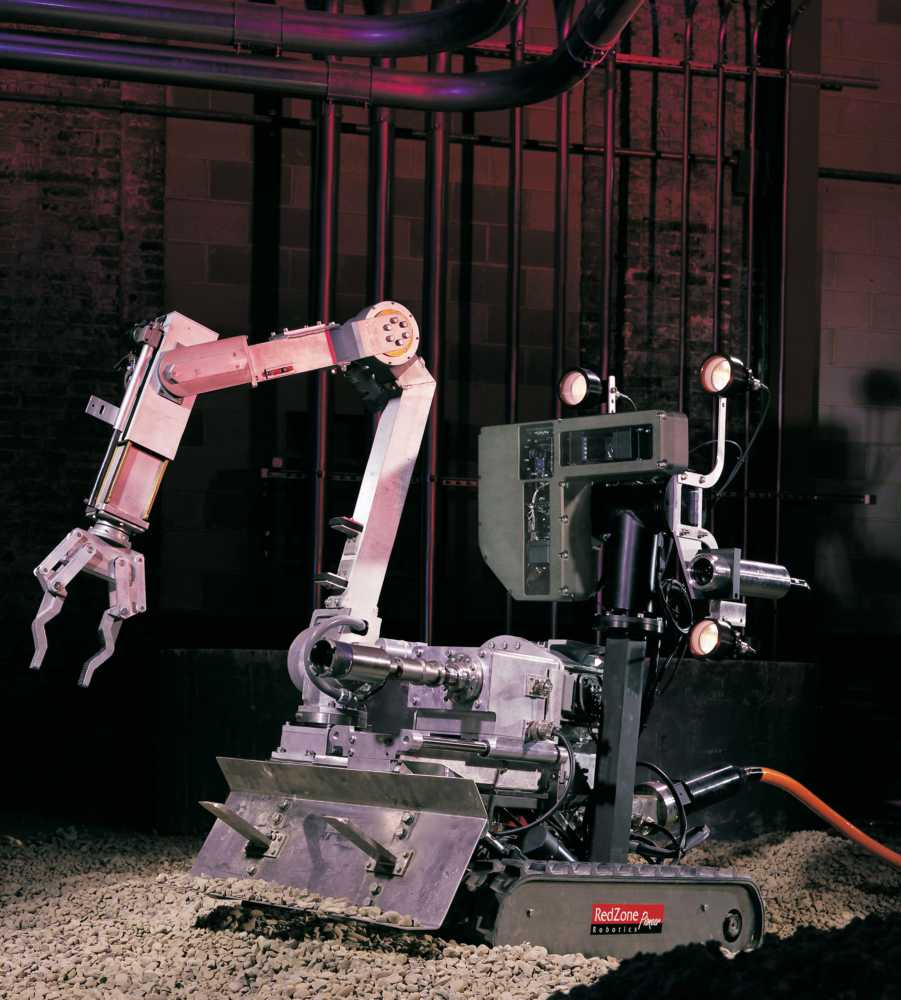
\includegraphics[width=0.8\linewidth]{images/pioneer_chernobyl}
			\caption{Pioneer robot, designed to perform hazardous teleoperated explorations in a deadly radioactive environment.}
			\label{fig:1_pioneer}
		\end{subfigure}
		\hfill
		\begin{subfigure}[b]{0.4\textwidth}
			\centering
			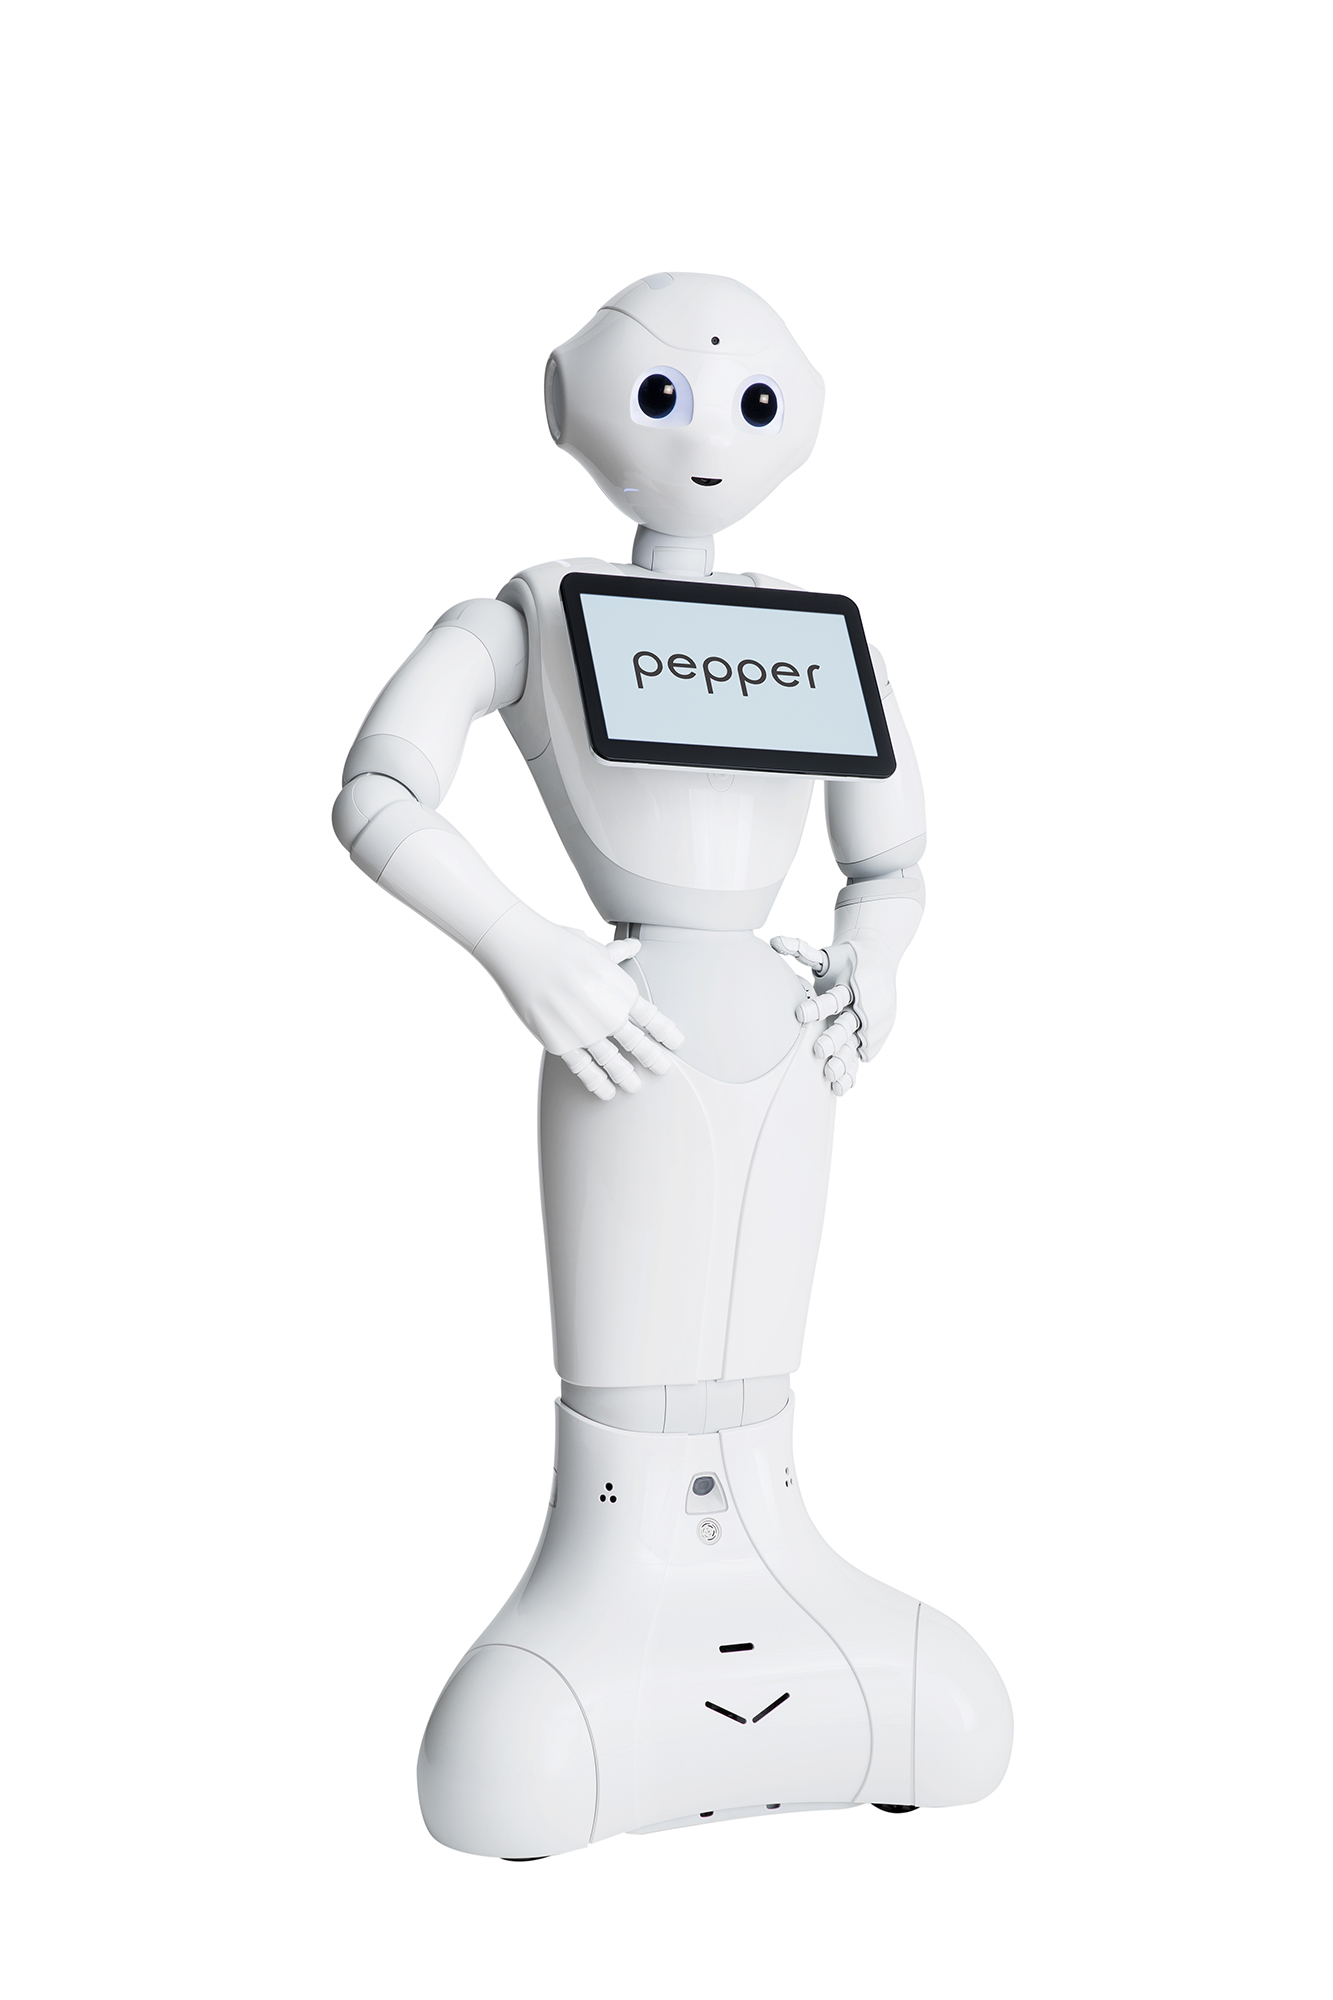
\includegraphics[width=0.8\linewidth]{images/pepper}
			\caption{Pepper, an autonomous humanoid capable of performing on board processing and reaction to external stimuli on a human way.}
			\label{fig:1_pepper}
		\end{subfigure}
		\caption{Robots of each described kind.}
		\label{fig:1_robots}
		
	\end{figure}

The important advances on the last decades on the image processing and audio recognition fields have impulsed the development of assistance systems, apart from critical machines as the previously described examples. \\

This way, several applications have arisen on people recognition and conversational behaviors, and it has been spread to everyday purposes, from personal assistants\footnote{\href{https://www.standard.co.uk/tech/google-smart-home-future-stay-a3868591.html}{Google Smart Home}}, to autonomous driving\footnote{\href{https://electrek.co/2018/06/18/what-tesla-autopilot-see-understand/}{Tesla Autopilot}}.\\


\section{Deep Learning}
\subsection{Machine Learning on Computer Vision}
Almost every time, the desired behavioral is one or more deliberated or reactive responses\footnote{A \emph{deliberated} response implies a certain level of \emph{extra intelligence}. It figures out which could be the best action to perform, considering present, past and probably future information to make the decision.\\ On the other hand, a \emph{reactive} response makes an immediate decision, depending just on what has been just perceived.}, triggered by a certain input (typically perceived by on-board sensors, among others). This raw data, which is typically retrieved on a simple way (images, audio), is processed and mapped into a concrete response. At this point, we can bring up the key question: \emph{how do we process the raw input to obtain a suitable action for the current requirements, or needings?} The answer for that question is \textit{machine learning}: the computer science field that pursues the capacity of machines to learn the suitable response to a previously unknown input. This is achieved by performing a training with a dataset of examples, which need to be properly formatted: the system has to previously know what to look for and evaluate, what is typically called \textit{features}, and learn the proper parameters for an optimum output.\\

Generally, machine learning applications on image processing can be split into two types of response (\autoref{fig:1_class_vs_det}):

\begin{itemize}
	\item \textbf{Classification:} given a set of possible classes $\{c_1, c_2, ..., c_n\}$ to which an image $x_i$ can belong, we select the class $c_i$ where $x_i$ fits the best, given a set of features extracted from it.
	\item \textbf{Detection}: given an image $x_i$, we decide if we can find or not an object/region inside of it which fits into the searched type. In the affirmative case, we locate it (using a region or a bounding box).
\end{itemize}

\begin{figure}[h!]
	\centering
	\begin{subfigure}[h!]{0.7\textwidth}
		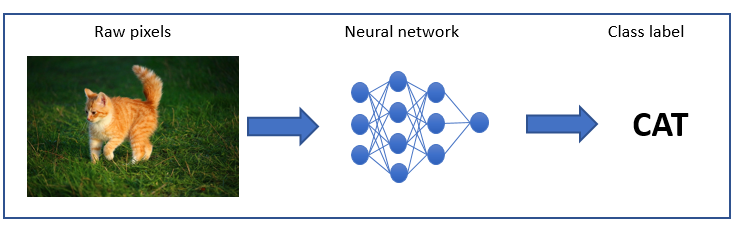
\includegraphics[width=\textwidth]{images/classification}
		\caption{Classification}
		\label{fig:1_classification}
	\end{subfigure}
	
	\qquad
	
	\begin{subfigure}[h!]{0.7\textwidth}
		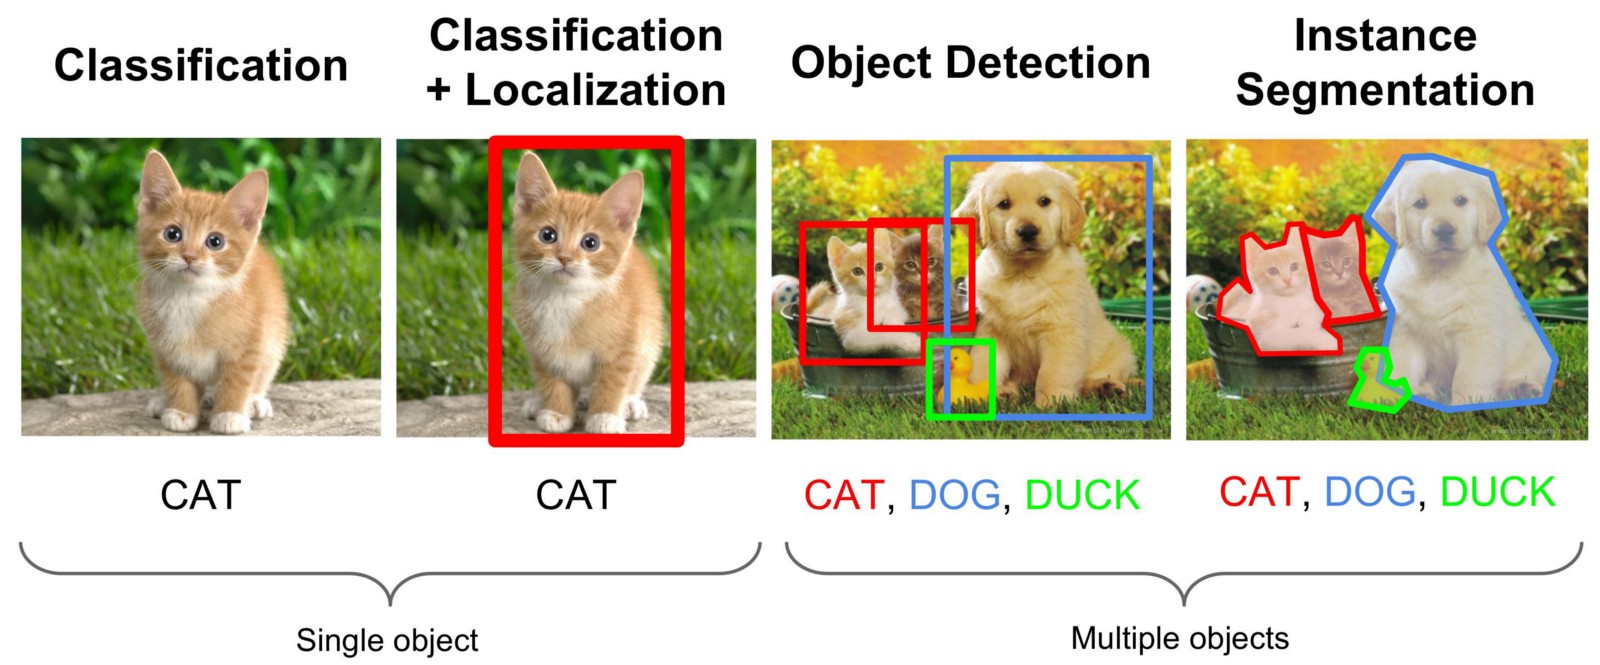
\includegraphics[width=\textwidth]{images/detection}
		\caption{Detection}
		\label{fig:1_detection}			
	\end{subfigure}
	
	\caption{Functional difference between \textit{classification} and \textit{detection}.}
	\label{fig:1_class_vs_det}
\end{figure}


\subsection{Neural Networks}
This has turned deep learning into the cornerstone of current \emph{AI} applications, which don't need complex dataset with a lot of preprocessing (that require important human effort) anymore. That simplicity is achieved through the use of \emph{Neural Networks}. A Neural Network is the representation of an algebraic algorithm which implements non-linear calculus models \cite{dl-nature}. It is composed by several processing \textit{layers}, which are made up of \emph{perceptrons}, that are generally called \textit{neurons}. This is because these neural structures \textit{emulate the human brain}, formed by a huge set of interconnected neurons, which are disposed on the already mentioned layers (\autoref{fig:1_neural_network}).\\

\begin{figure}[htpb]
	\centering
	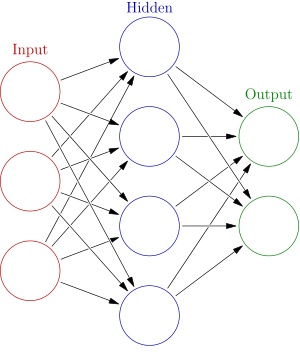
\includegraphics[width=5.5cm]{images/neural_network}
	\caption{Structure of a Neural Network}
	\label{fig:1_neural_network}
\end{figure}

First approaches to neural networks, according to \cite{nn-history} were developed on the 50s-60s decades. This was when the computational potential allowed to develop on a real machine the first modeling of the way it was believed that a brain neuron works, which was inspired by electrical circuits. These experiments \cite{first-neuron} were performed by the neurophysiologist W. McCulloch and the mathematician W. Pitts. Later, in 1949, Donald Hebb \cite{hebb} observed that the synaptic path between two neurons is reinforced (its efficiency rises up) every time it is used. This introduced the concept of \textit{training} on a neural network.

\subsection{Processing unit: the perceptron (neuron)}
\begin{figure}[h]
	\centering
	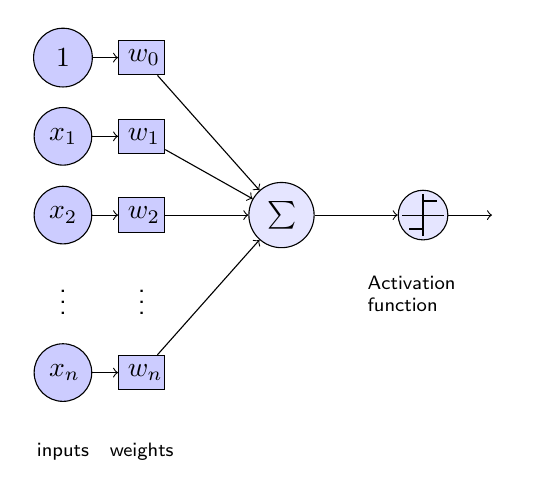
\begin{tikzpicture}
	\node[functions] (center) {};
	\node[below of=center,font=\scriptsize,text width=4em] {Activation function};
	\draw[thick] (0.5em,0.5em) -- (0,0.5em) -- (0,-0.5em) -- (-0.5em,-0.5em);
	\draw (0em,0.75em) -- (0em,-0.75em);
	\draw (0.75em,0em) -- (-0.75em,0em);
	\node[right of=center] (right) {};
	\path[draw,->] (center) -- (right);
	\node[functions,left=3em of center] (left) {$\sum$};
	\path[draw,->] (left) -- (center);
	\node[weights,left=3em of left] (2) {$w_2$} -- (2) node[input,left of=2] (l2) {$x_2$};
	\path[draw,->] (l2) -- (2);
	\path[draw,->] (2) -- (left);
	\node[below of=2] (dots) {$\vdots$} -- (dots) node[left of=dots] (ldots) {$\vdots$};
	\node[weights,below of=dots] (n) {$w_n$} -- (n) node[input,left of=n] (ln) {$x_n$};
	\path[draw,->] (ln) -- (n);
	\path[draw,->] (n) -- (left);
	\node[weights,above of=2] (1) {$w_1$} -- (1) node[input,left of=1] (l1) {$x_1$};
	\path[draw,->] (l1) -- (1);
	\path[draw,->] (1) -- (left);
	\node[weights,above of=1] (0) {$w_0$} -- (0) node[input,left of=0] (l0) {$1$};
	\path[draw,->] (l0) -- (0);
	\path[draw,->] (0) -- (left);
	\node[below of=ln,font=\scriptsize] {inputs};
	\node[below of=n,font=\scriptsize] {weights};
	\end{tikzpicture}
	\caption{Diagram of a perceptron/neuron}
	\label{fig:1_perceptron}
\end{figure}

\vspace{0.3in}
Every neuron is composed by an structured schema:
\begin{enumerate}
	\item \emph{Inputs}: the data which come into the neuron. It might come from the main stimuli, or from another neuron (as the output of the previous layer). The input for a specific neuron is called its \emph{receptive field} (which region of the total input that stimulates that particular neuron, where it looks for features).
	\item \emph{Weights}: the tuned parameters of the network. They represent the importance given to each feature on that singular neural unit. The weight $w_n$ multiplied $x_n$ times results on the contribution of the feature $n$ in the current neuron. 
	\item \emph{Sum}: the product of all the inputs with their suitable weight come into a sum operation\footnote{We consider $w_0$ as the product to the constant input $1$, as the intercept term (a constant always present independently of the current input).}, to \textit{build a total linear response:} $ z = \sum_{i=0}^{n}x_i \cdot w_i$  \footnote{There is also a summation bias term on each neuron, $b_i$, but it is ignored here for the sake of simplicity, as the weights are more representative with respect to the input.}.
	\item \emph{Activation function}: this is an crucial part of a neural network. Until now, all the numerical computations we have performed were just linear operations. If we keep the output of the neuron being a linear function of the input, we will lose the effect of having more than 1 layer, as really the total result of all the network is a linear function of the first input, so \emph{we could simplify all the network down to one single neuron}. \\
	
	For this reason, we use a \textit{non-linear activation function}, which breaks the linearity on the pipeline to provide the absolute non-linearity followed by the human brain. A typical function is the one called \emph{ReLU} (REctified Linear Unit) \cite{relu}, which follows the formula:
	\begin{equation}
		g(z) = max(0, z)
		\label{eqn:1_relu}
	\end{equation}
	
	\item \emph{Output}: when the activation function has been computed, it is forward-propagated to the output, or to the neurons belonging to the next layer. It can be seen as the importance that particular feature will have on the next neuron: if it takes nearly zero values, the next neuron will be poorly stimulated. There lies the meaning of the name of the previous component: \emph{activation function}.\\
	
	As a conclusion, we can find that the general output of a neuron $a(z)$ as:
	\begin{equation}
		a(z) = g(\sum_{i=0}^{n}x_i \cdot w_i)
	\end{equation}
	
	This will be the new data (\emph{receptive field}) that will be introduced on a neuron or set of them from the next layer.
\end{enumerate}

\subsection{Deep Neural Networks}

\emph{Deep learning} is the piece of machine learning that is capable to \textit{automatically learn the features that the system could use from primary data} (pixels on images, samples on audio, words in text processing, etc.).\\

The fact of having more than one layer gives to the network the concept of \emph{depth}. This opens the door to a vast set of possibilities, as \textit{it allows us to perform deep learning with neural networks: Deep Neural Networks}. This can be achieved, as we can see on \autoref{fig:1_deep_nn}, by introducing a new kind of layer, where all the new neurons are connected to every single neuron of the previous one.\\
This is typically called a \textit{fully connected layer}, and the fact of relating every single activation from the previous layer with a set of tunable weights on each neuron allows to rapidly find common patterns followed by features seen on one of the analyzed scenarios (e.g. syntactical relationships between several kinds of words in language processing, or finding edges or shapes on image detection/classification).

\begin{figure}[h]
	\centering
	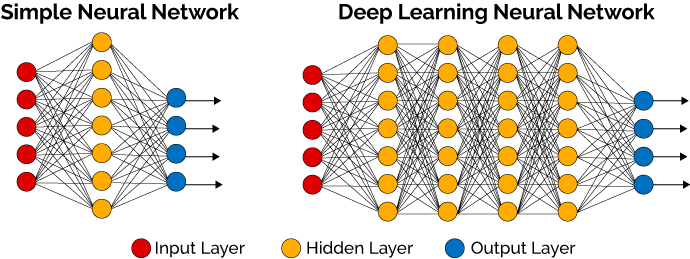
\includegraphics[width=0.9\linewidth]{images/deep_neural_network}
	\caption{Evolution to a \textit{deep} neural network.}
	\label{fig:1_deep_nn}
\end{figure}

\subsection{Convolutional Neural Networks (\emph{CNNs})}
\label{sec:1_cnn}

Finally, this leads us to the last concept we will study on this dissertation. As we have said before, we can connect a big set of neurons between themselves to extract more abstract and complex features, of increasing interest with the number of neurons and layers.\\
 
If we aim to apply this processing to images (\textit{Computer Vision}), we have to take into account that, if we want to input an image into a neural network, each pixel has to be taken as an input, and also the fact that an RGB image is composed of 3 channels (1 channel per color), so, for an image with a dimensions of $m$ pixels wide and $n$ pixels high, we will need $m\cdot n \cdot 3$ input neurons. Besides this considerable number, we will have to take into account the neurons resulting on the additional deeper layers that we will add to have an high enough abstraction level for our application. This drives to absurd numbers of simultaneous neurons working, that are difficultly handable during a feed-forward execution, but absolutely unfeasible on a training process. An additional problem can be a moving object/region on the image: we must be capable to detect the shape of a car on the right side of the image, or in the left one.\\

We can solve both problems simultaneously with an easy procedure: we will not process the entire image at one time. Instead of that \textit{we will perform a convolution operation (\autoref{fig:1_convolution}) between the inputs of our network, and different regions of the image}, sliding and multiplying a \emph{parameterized mask} along the whole image. This operation is performed with the objective of the product returning a high value on the interesting regions of the image. This will output \emph{activation maps}, which symbolize the response of that portion of the image to the weight mask. This can be performed, as we have said before, a few times with different masks to obtain features with a higher degree of abstraction. As we want to keep the computational complexity low, we can alternate these layers with \textit{pooling layers}, which subsample the resulting maps, to keep it simple (if we keep only 1 of each 3 pixels of an activation map, selecting it carefully to retain the maximum information, we can reduce the number of necessary neurons on the next layer on a factor of $\frac{1}{3} \cdot \frac{1}{3} = \frac{1}{9}$). This is reflected on \autoref{fig:1_cnn}, where the process of convolution-pooling can be repeated a few times, and then the result (which should not have considerably big dimensions) are inputted into a fully connected layers, to extract and handle the relations between the features and the possible classes (on a classification scenario).\\


\begin{figure}[h]
	\centering
	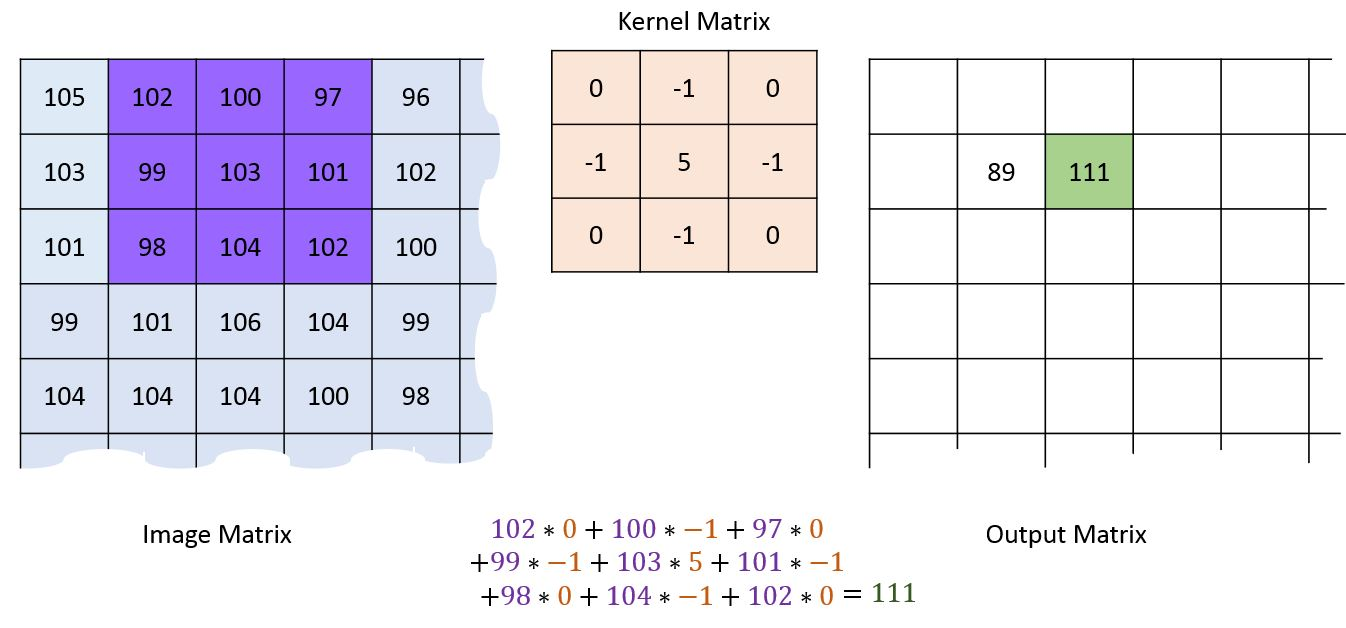
\includegraphics[width=5in]{images/convolution}
	\caption{Convolution operation applied on an image (image from \cite{image-convolution}).}
	\label{fig:1_convolution}
\end{figure}





But, \emph{how do we find the best value for each weight, and for each layer?} That's the process we call \textit{training a network}. Using a technique called \emph{back propagation}, we can compute the most suitable values for every neuron in the network.\\

\begin{figure}[h]
	\centering
	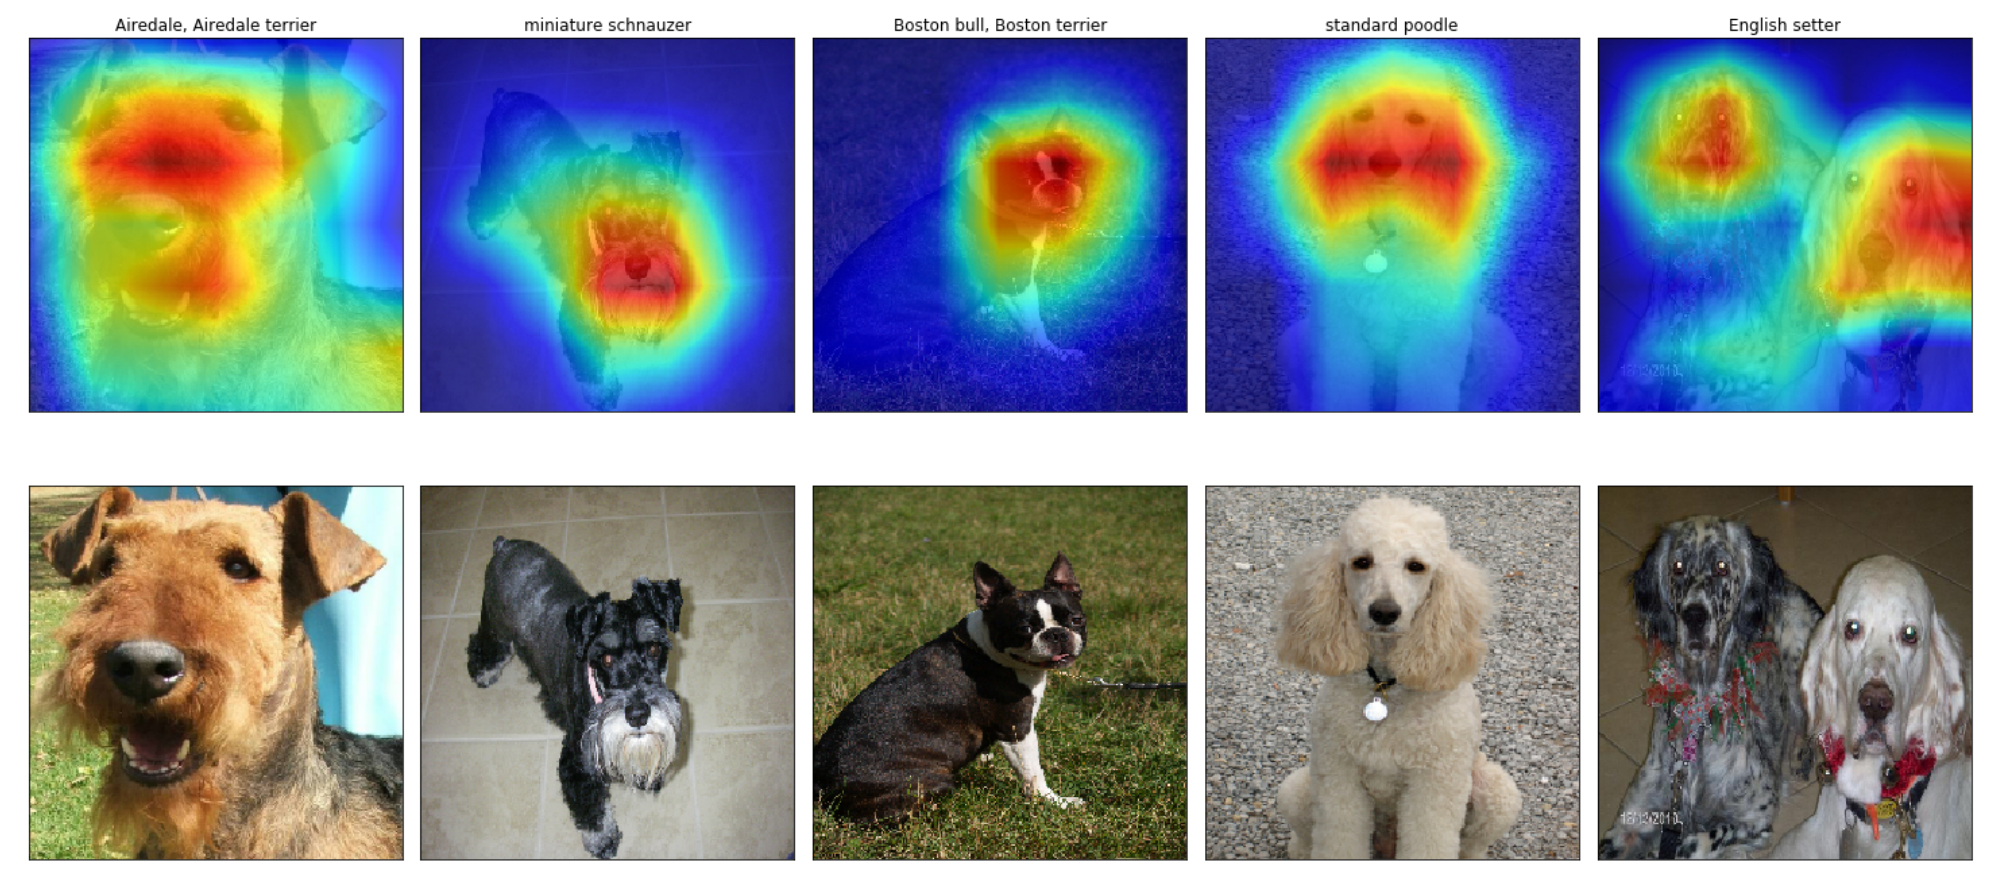
\includegraphics[width=0.9\linewidth]{images/activation_maps}
	\caption{Activation maps of a detection CNN searching for dogs on different images \cite{activation-maps}.}
	\label{fig:1_activation_maps}
\end{figure}



\begin{figure}[h]
	\centering
	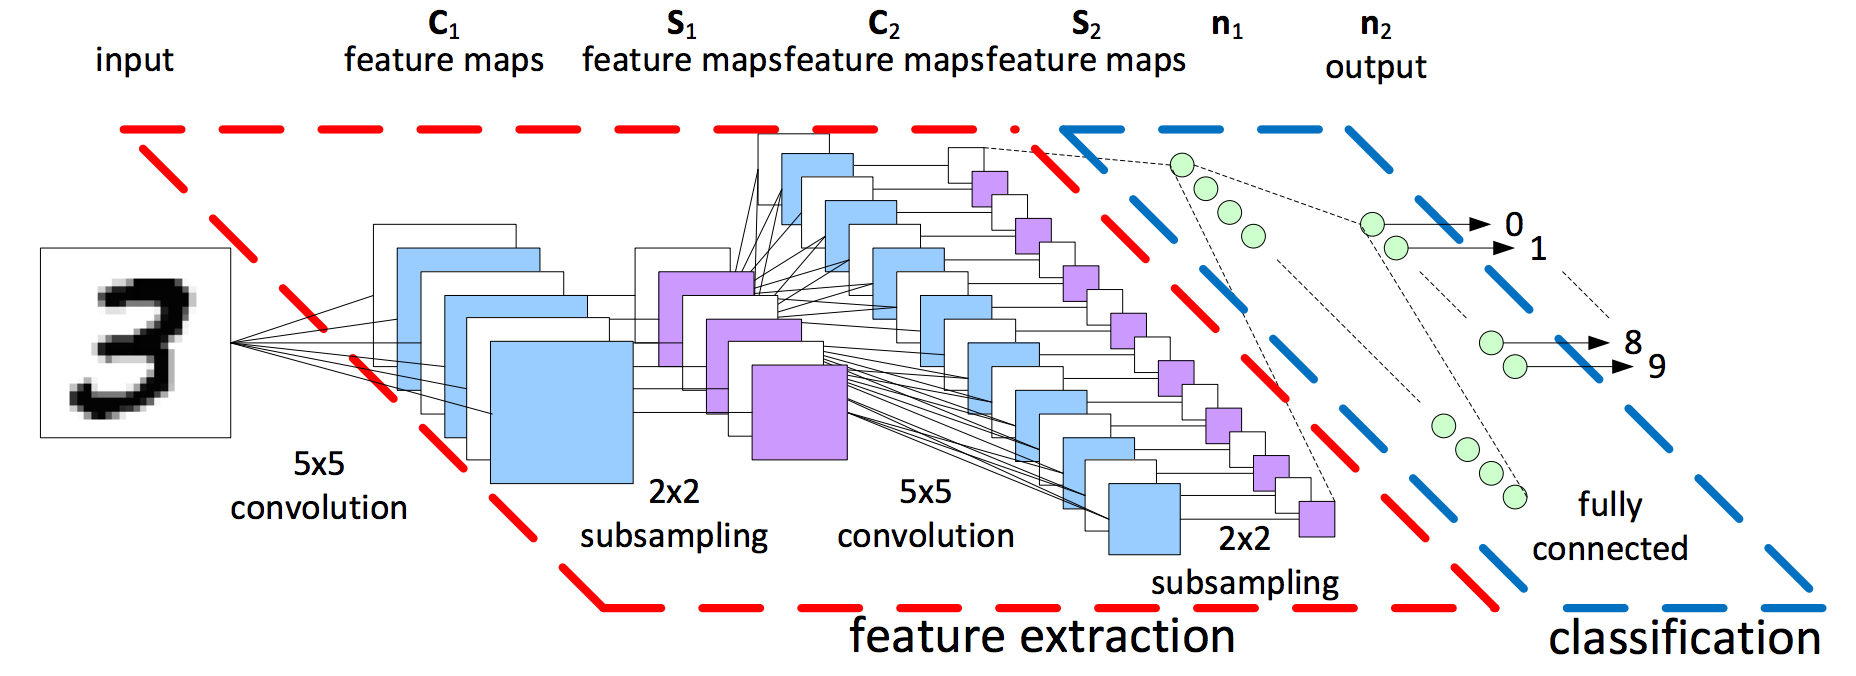
\includegraphics[width=0.9\linewidth]{images/cnn}
	\caption{Schematic of a CNN.}
	\label{fig:1_cnn}
\end{figure}

\section{Deep Learning on JdeRobot}
\label{sec:dl_jderobot}
So, as we have been describing, Deep Learning can be of a great interest on the image processing field, as it allows to implement an easy and really robust AI algorithm.\\

JdeRobot\footnote{\url{https://jderobot.org}} is an open-source software development suite, built from  this University, and among all the developed software/investigation inside it, we can find some interesting programs/projects for our purposes:

\begin{itemize}
	\item \texttt{Detection Suite}\footnote{\url{https://github.com/JdeRobot/dl-DetectionSuite}}: it is a C++ application, suitable to load/benchmark \textit{detection} Darknet/YOLO\footnote{\url{https://pjreddie.com/darknet/}} models, against different databases. It is also capable, through a Python$\rightarrow$C++ interface, to load TensorFlow/Keras models as well.
	
	\begin{figure}[h]
		\centering
		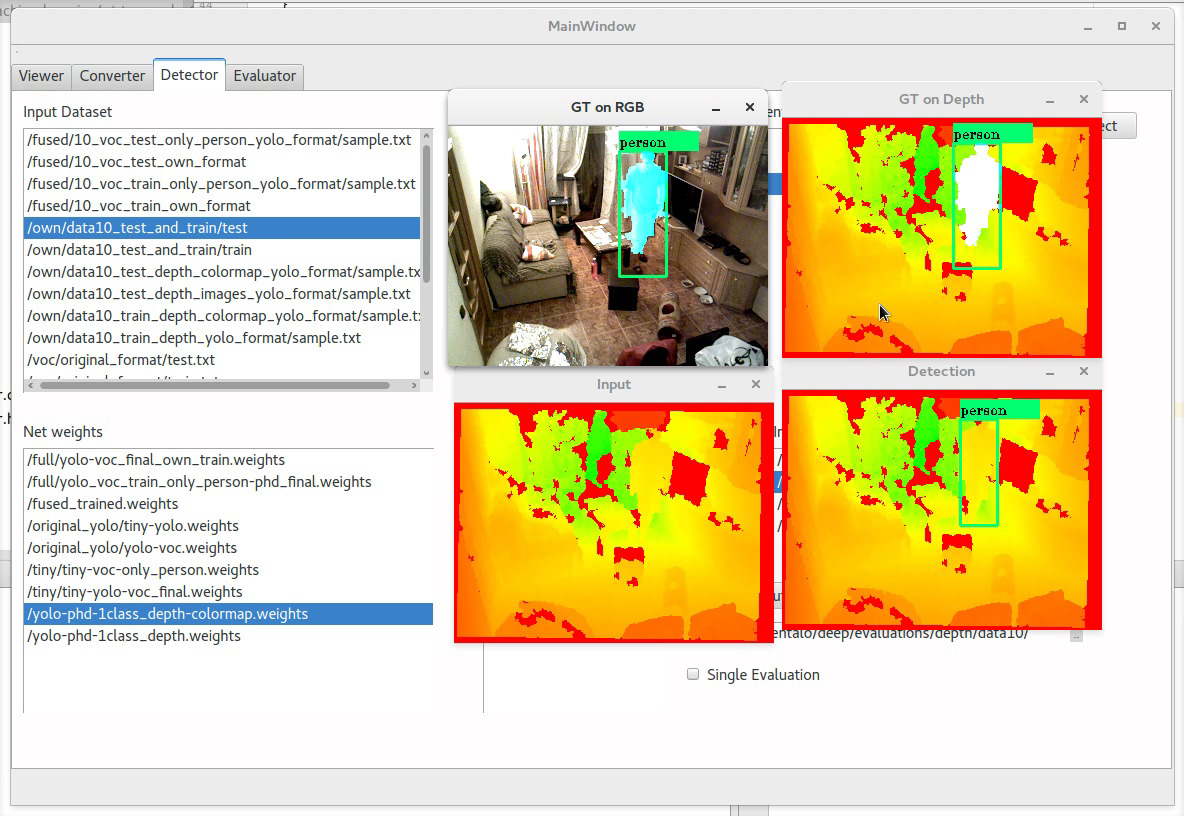
\includegraphics[width=4.5in]{images/detection_suite_depth}
		\caption{\texttt{DetectionSuite} on action.}
		\label{fig:1_detectionsuite}
	\end{figure}

	\item Final project of David Pascual \cite{dpascualhe} and Nuria Oyaga \cite{noyaga}: a further study of Deep Learning, applied on Python (Keras and Caffe frameworks, respectively) to \textit{digit classification} (\autoref{fig:1_digitclassifier}) implementing a CNN as it has been seen.
	
	\begin{figure}[h]
		\centering
		\begin{subfigure}[h]{0.45\linewidth}
			\centering
			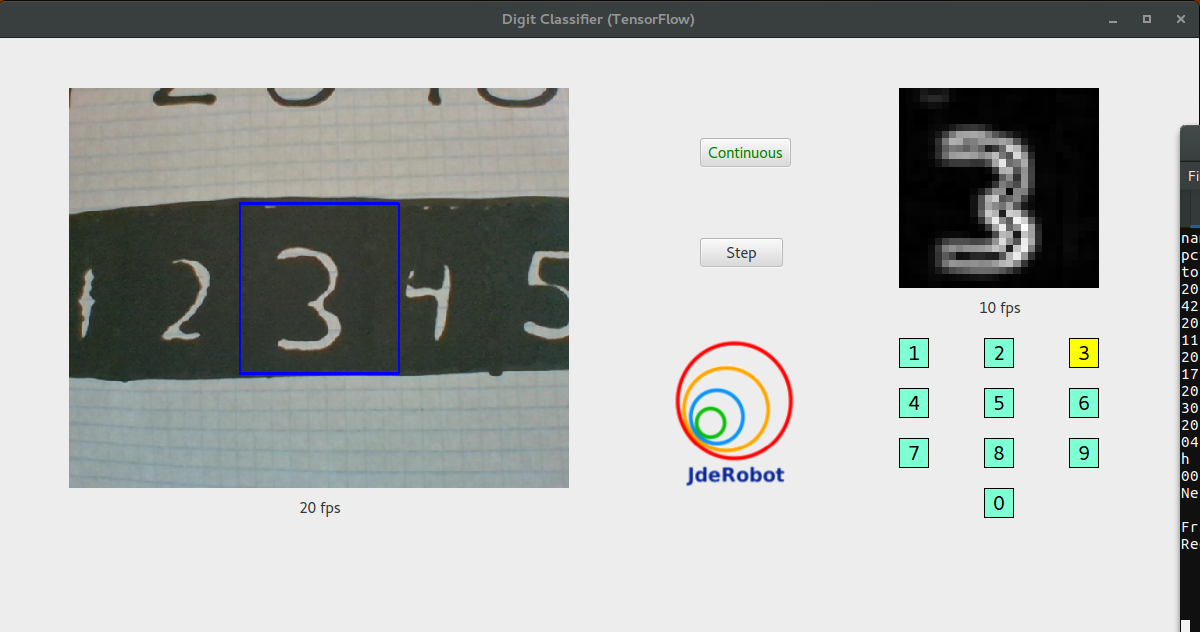
\includegraphics[width=2.7in]{images/digitclassifier}
			\caption{\texttt{DigitClassifier} working.}
			\label{fig:1_digitclassifier}
		\end{subfigure}
		\qquad
		\begin{subfigure}[h]{0.45\linewidth}
			\centering
			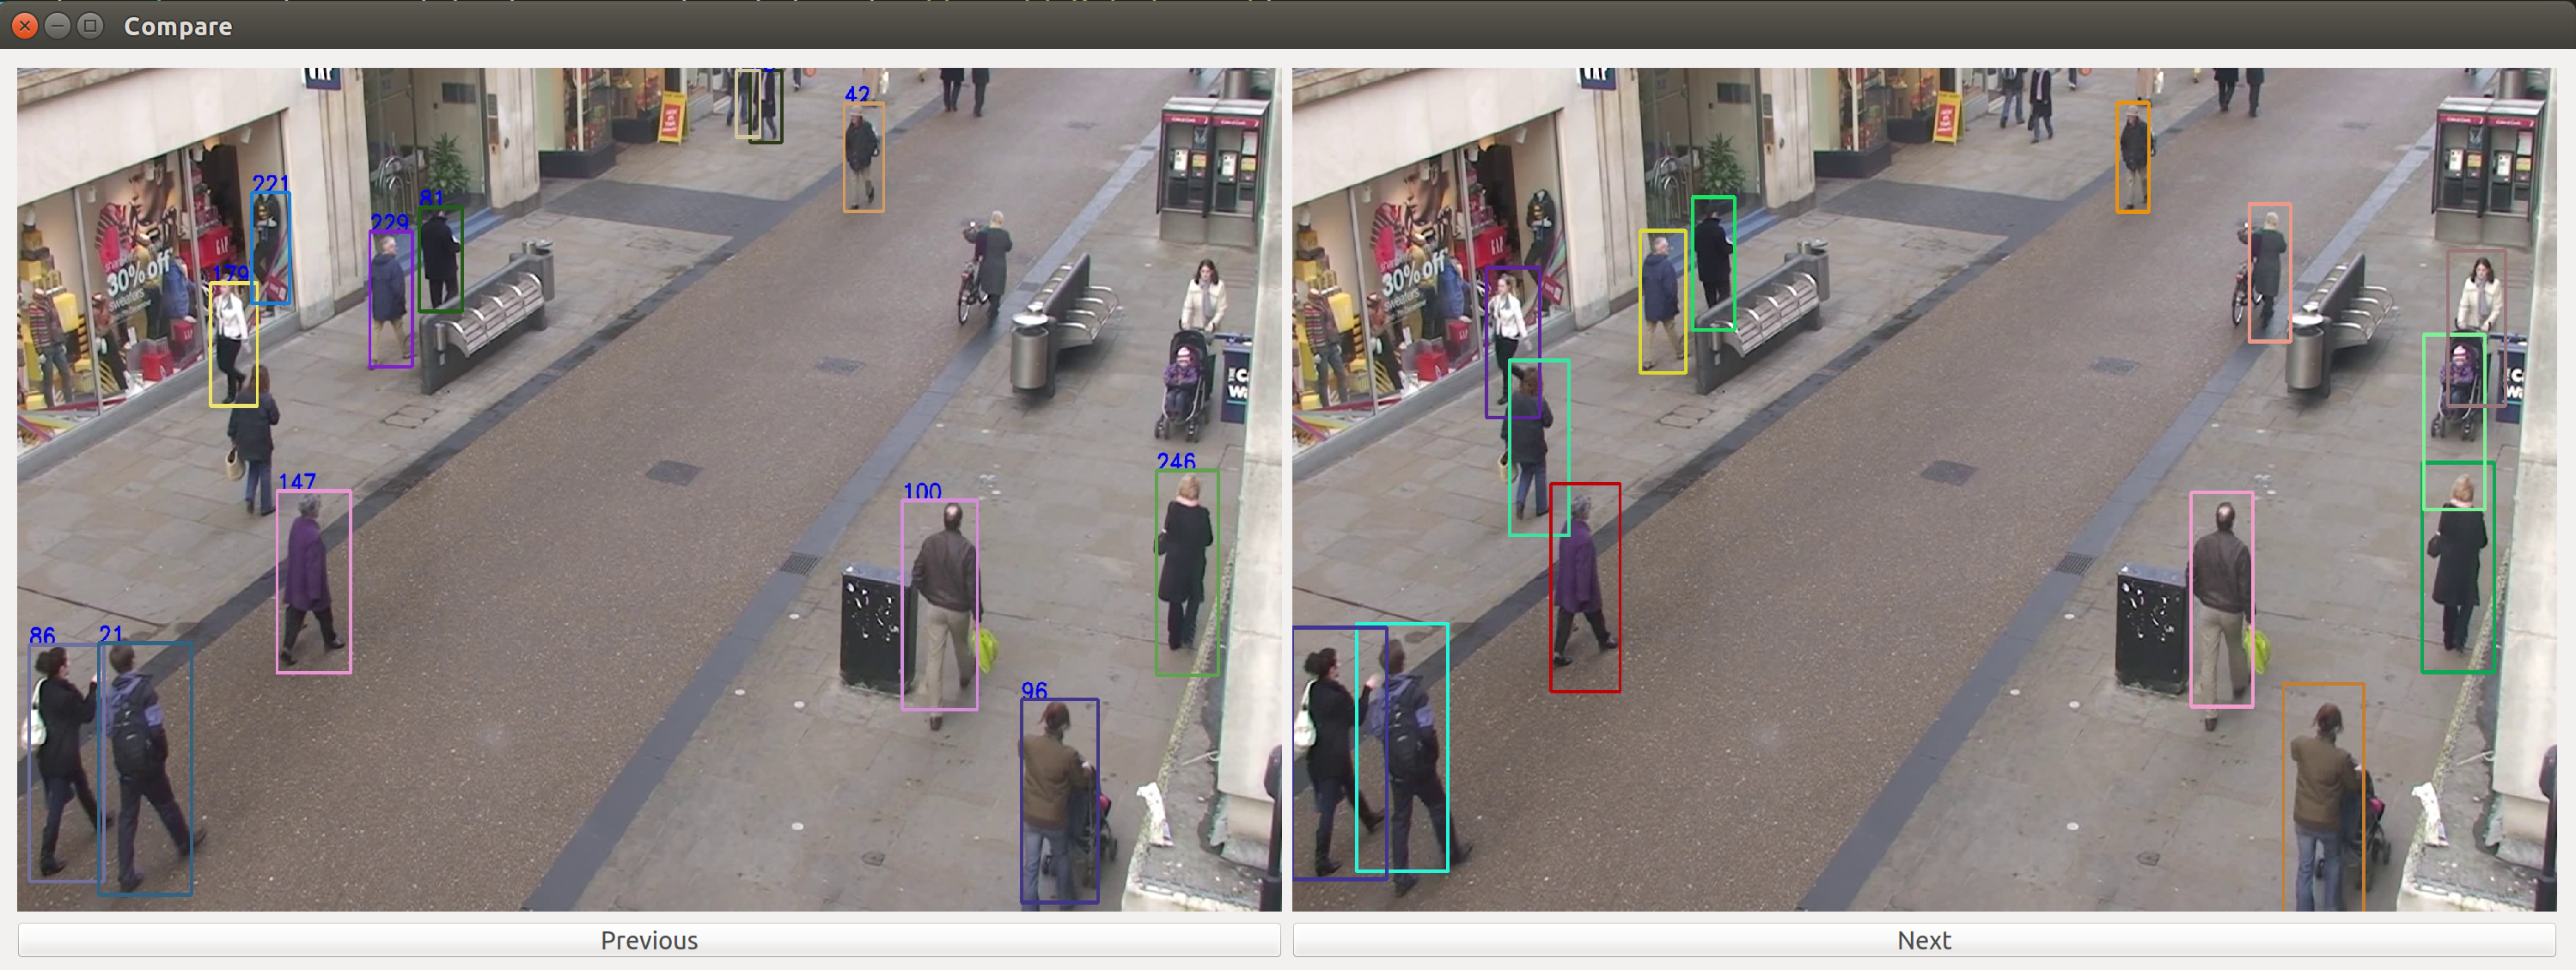
\includegraphics[width=3.7in]{images/marcos_people_tracker}
			\caption{\texttt{PeopleTracker} working.}
			\label{fig:1_people_tracker}
		\end{subfigure}
		\caption{Some JdeRobot student projects on action.}
		\label{fig:1_jderobot_projects}
	\end{figure}

	\item MsC project of Marcos Pieras \cite{marcospieras}: On this master thesis, an application implementing two neural networks (as we will do) has been developed. One of them allows us to \textit{detect} people on an image, and the other one (a siamese network, as we will describe later) can track features of each person, to keep every detected individual identified on a surveillance image system (and possibly trace the route followed by each person) (\autoref{fig:1_people_tracker}).
\end{itemize}

In conclusion, as we have been mentioning and been taking a glance on the possible applications, Deep Learning can make such a brilliant tandem along with a reactive behavioral. We have taken a glance on a few possible applications, and the following dissertation will struggle to demonstrate it.\\




\begin{center}
	\textbf{Robotics + deep learning rock!}
\end{center}



	

	
	
	
	%%%%%% OBJECTIVES %%%%%%
	\chapter{Objectives}
Once we have presented the introductory context of this project, we will describe its objectives, along to the followed methodology to achieve all of them.\\

The final objective is to enrich the JdeRobot platform on its Computer Vision aspect, upgrading an existing component and creating two consecutive new ones. Keeping this in mind, we will be able to generate a behavioral focused, as a specific application, on tracking and actively following a person, making use of a robot. This internal process of transformation of the stimuli into a reactive movement will be accomplished using \textit{Convolutional Neural Networks}.\\


\section{Main objectives}

		\subsection{Classification}
			Our first objective (and the first task to tackle) will be to upgrade the support of the digit classification tool already present in JdeRobot, \texttt{DigitClassifier} (\autoref{sec:3_digitclassifier_jderobot}). This will allow us to make the scope of this component bigger, due to the support for the new framework, TensorFlow (\autoref{sec:3_tensorflow}). This is a good starting point to achieve some initial skills building and training Convolutional Neural Networks on TensorFlow (it will be the main framework used all along the project).\\
		
		
		\subsection{Detection}
			As it will be described on the suitable chapter, we will build a component (\texttt{ObjectDetector}) which deploys \textit{a generic object detection algorithm} on an incoming video stream. This component will be ready to work in \emph{real time}. It will also be compatible with new network models (e.g. a new detection model trained by us), which will be loaded transparently at runtime.\\
			
			As it can be inferred, it will not provide a response \textit{per se}. Its visible output will be to draw \emph{bounding boxes} surrounding each detected object, indicating as well the class where that particular object belongs (person, airplane, dog, etc.), and its score (confidence in \%).\\
		
		\subsection{Tracking and following}
			As an example of the plethora of possible applications of the previous described objective/milestone (object detection on an image), we want to implement a ``person following" behavioral. Our main objective here is to \textit{identify and track} the person to follow, which will semantically be called \emph{mom}. The component that comprehends the previous detection behavioral and this new one will be named \texttt{FollowPerson}. The great advantage here is the strength a CNN can achieve under variable light conditions. That makes this technique perfectly suitable to command physical actuators on a robot.\\
			
			We will make use of the detected people (with the technique followed on the previously described node and constraining the result to only retain people detection), and look for the face of each one of them. Later, we will make use of another neural network technique, called a \emph{siamese network} (it will be properly explained later) to identify them. It will allow us to find \emph{mom}, in case it is being seen by the camera, and command a proper response to the robot with the objective of following \emph{mom}.\\
			
			\vspace{1in}

As we have said before, these two last nodes/components are successive. Thus, they will share an important part of the global objectives.\\

We will start breaking down the common objectives between both applications, into three functional blocks:

\begin{itemize}
	\item \textit{Design:} both milestones have been preceded by a first \textit{documentation} phase. While the theoretical base was learned and achieved, some papers and examples were investigated. We will go some deeper in each section.
	
	Later, a more specific design phase will be to specify the structure of the nodes.
	From now on, we will have to perform several tasks simultaneously:
	\begin{itemize}
		\item Grabbing the incoming image(s) from the sensor(s).
		\item Processing the image(s).
		\item Properly update the GUI (\textit{Graphical User Interface}) with the image(s) and the outputs of the processing.
		\item \textit{Only on the following node:} send the computed response order to the actuators.
	\end{itemize}
	%
	These tasks should follow an \emph{asynchronous schema} every time, to avoid blocks between tasks, and taking advantage of some shared memory to exchange inputs/outputs. Besides, this allows us to have a custom iteration period for each task: we shouldn't have to wait until the neural network finishes feed-forwarding the image to refresh the \emph{GUI}. On a high level structure, it could follow the schema on the \autoref{fig:2_tasks}.
	
	\begin{figure}[h]
		\centering
		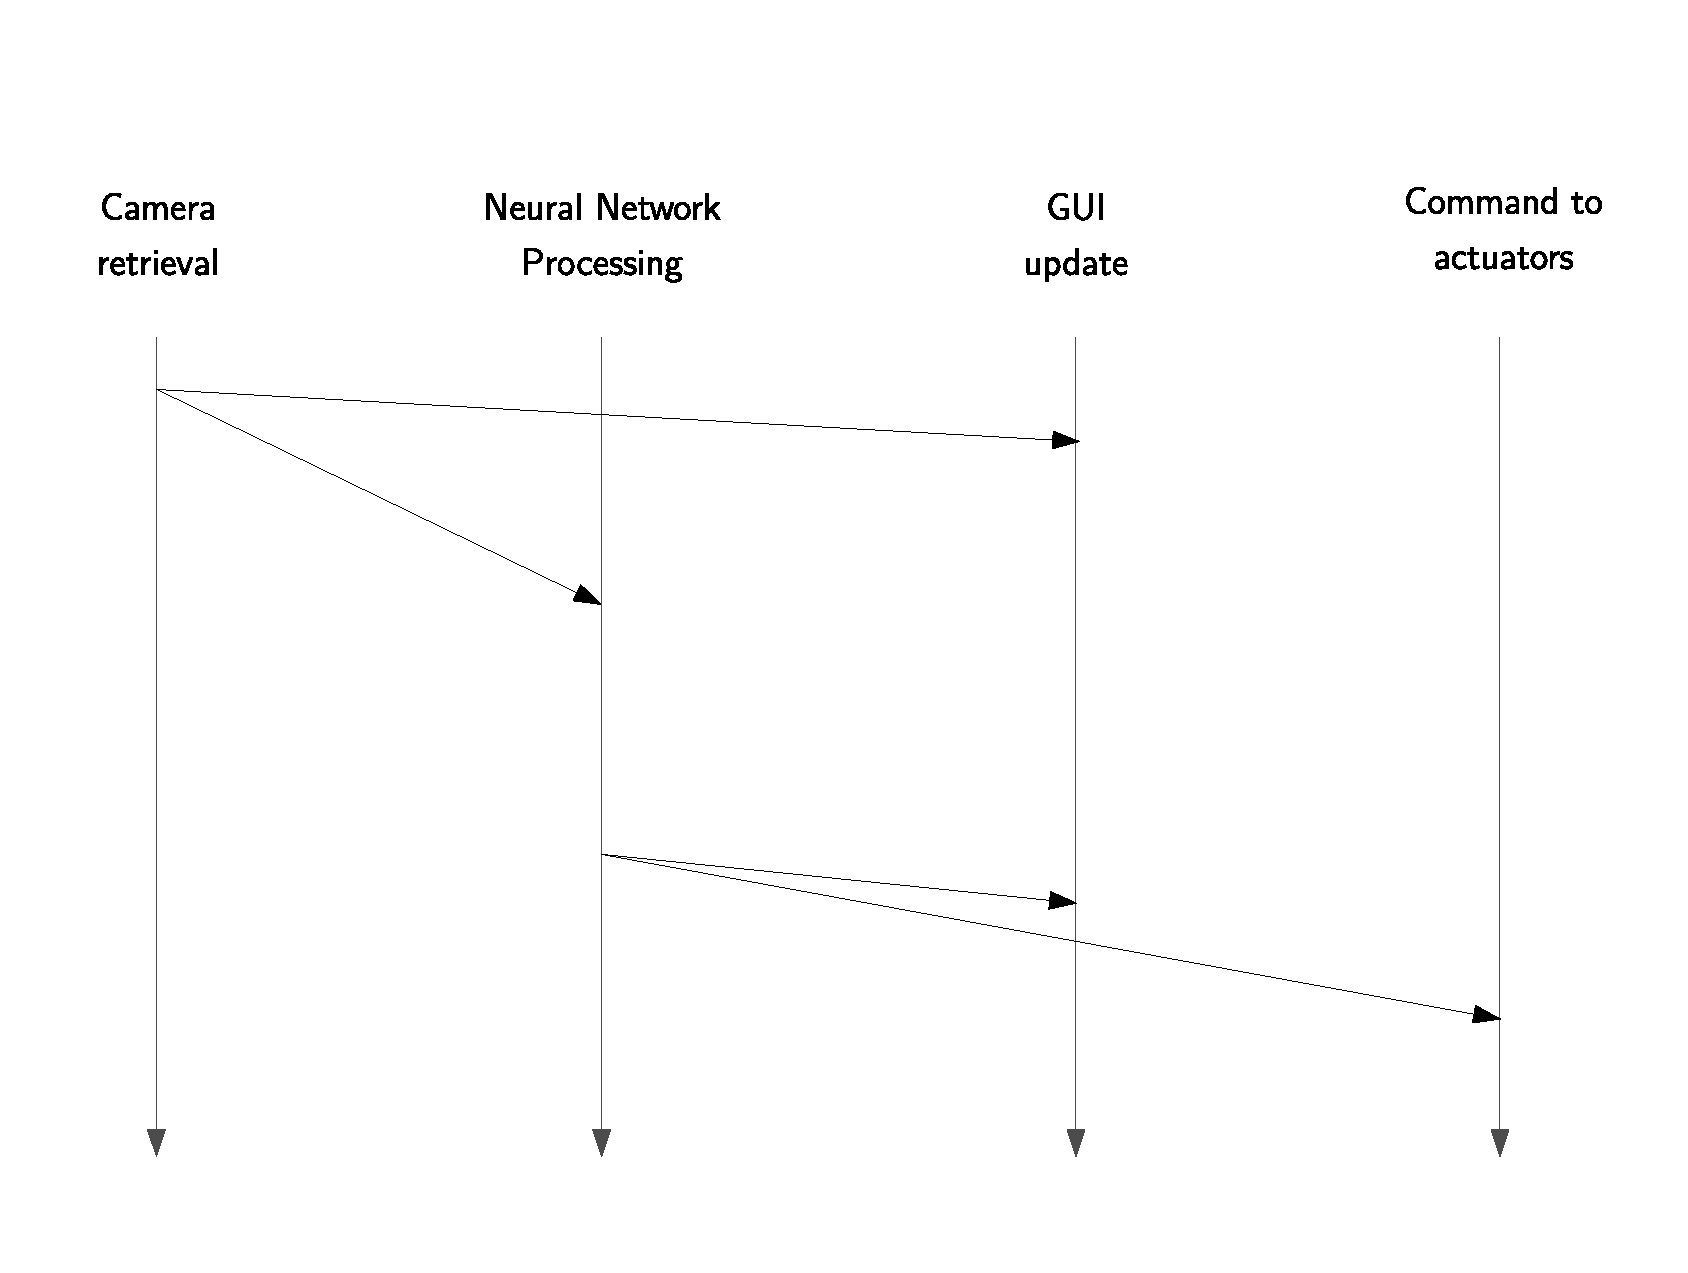
\includegraphics[width=4in]{images/tasks_threads}
		\caption{Parallel tasks to perform, and data exchange between them.}
		\label{fig:2_tasks}
	\end{figure}
	
	\item \textit{Implementation:} the next and most time consuming objective is to \textit{develop both components}. The advantage is, once again, that both components are successive. This makes code reutilization a very interesting move, as we will only need to perform a language-friendly additions (on a simple way, thanks to \textit{Object Oriented Programming})) to the \texttt{Object Detector} code to implement the \texttt{Follow Person} features (depth images support, computing and commanding movements to the motors, among others). Details will be described on the appropriate section.
	
	\item \textit{Experimentation\footnote{\textit{"In theory, theory and practice are the same. In practice, they are not."}, Y. Berra}:} these nodes have a very strong tunability component (from neural network parameters to movement factors in the commands for the motors, stopping over describing all the desired behavior that the following algorithm has to adopt in several situations that it has to be capable of handling).
	
\end{itemize}

Finally, we will briefly highlight the \textit{personal} objectives we have pursued on this project. As this has been developed along a whole year, and on a relatively abstract field as \emph{deep learning} is, a level of rigour has been necessary to accomplish satisfactory results. This provides a novice investigator the opportunity to learn about the phases and development process on a much more professional way than a homework task. \\

In addition, this project has allowed an interested person in \emph{deep learning} to learn about a cornucopia of concepts and experience. Later, when it was decided to evolve towards creating a reactive behavioral, it was motivating to make the most of a possible synergy between two different fields of knowledge, as \emph{deep learning} and \emph{robotics} are. It has to be remarked that the implementation of the development has always been possible, so it has been easy where there was more work to do in every moment.

\section{Methodology}
The development of this project, as it has been described, has been subdivided into smaller tasks, or \emph{prototypes}, which could be addressed as individual tasks to achieve. The way to tackle them has been a \textit{spiral methodology} \cite{boehm-spiral}.\\

\begin{figure}[h]
	\centering
	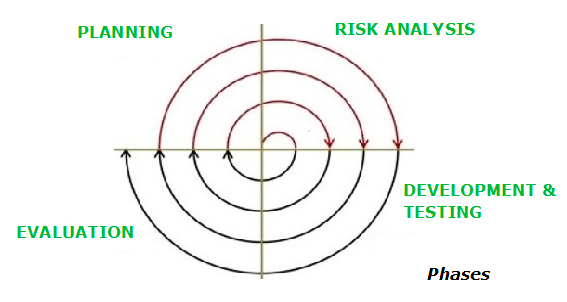
\includegraphics[width=4in]{images/spiral}
	\caption{Spiral Development Model.}
	\label{fig:2_spiral}
\end{figure}

This consists on a software development work procedure that, on a general outline, is very similar to a conch. It describes a 4 phases methodology \cite{spiral-steps}, explained right below:

\begin{enumerate}
	\item \textit{Planning:} establishing the objectives to tackle on the incoming work iteration.

	\item \textit{Risk Analysis:} Later, we evaluate the possible risks and dangers we can find developing the specific program(s). For each found risk, we will try to find a solution to solve or, at least, mitigate it beforehand.

	\item \textit{Development \& testing:} This phase is purely focused on writing the planned piece of software, following the guidelines obtained on the previous steps. In addition, corresponding tests should be performed to check that the work will accomplish the asked functionality.
	\item \textit{Evaluation:} Lastly, when the development phase has been finished, an evaluation has to be performed on the results. This will be the key to know if it is compliant with the initial requirements and if, hence, its development has been successful.
\end{enumerate}

As this was the general procedure followed for each iteration of the developed software, the completion of the evaluation phase immediately led to another planning phase, already belonging to the next iteration. As this is a cyclic process, we can perform as many iterations as desired, slightly increasing the scope of the project on each new one.\\

The workflow present on this project has been supported by weekly meetings, scheduled in order to get up-to-date with the last established objectives and tasks, and set up the work until the next one. This has allowed to keep a constant feedback with the tutor and hold the followed path onto the desired direction.\\

Additionally, a MediaWiki page\footnote{\url{https://jderobot.org/Naxvm-tfg}} has been mantained on the JdeRobot website, reflecting every effort and achievement in order to have a good temporal reference of the work done, and a timeline of accomplishments, and including demonstration videos for each successful iteration result.\\

The code for all the project has been handled on the GitHub repository\footnote{\url{https://github.com/RoboticsURJC-Students/2017-tfg-nacho\_condes}} created for this purpose. However, as the resulting nodes were officially incorporated to the JdeRobot environment, they were migrated to their own repositories. This will be further described on the section dedicated to each component/iteration.\\

	
	%%%%% INFRASTRUCTURE %%%%%
	\chapter{Infrastructure}

\section{Hardware}
	\subsection{Sony EVI D100P}
		\begin{figure}[h]
			\centering
			\begin{subfigure}[h]{0.4\linewidth}
				\centering
				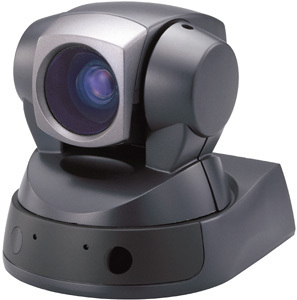
\includegraphics[width=1.6in]{images/ptz_front}
				\caption{Front side.}
			\end{subfigure}
			\qquad
			\begin{subfigure}[h]{0.4\linewidth}
				\centering
				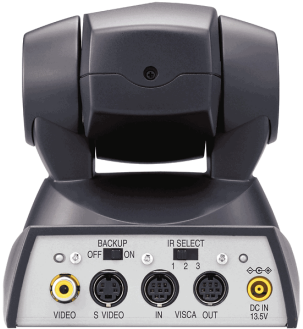
\includegraphics[width=1.6in]{images/ptz_back}
				\caption{Back side.}
			\end{subfigure}
			\caption{Sony EVI D100P.}
			\label{fig:3_evi}
		\end{figure} 
		
		The first hardware element that we used is the Sony EVI D100P\footnote{\url{https://pro.sony/en_IN/products/ptz-network-cameras/evi-d100-d100p-pal-}}. It is a \emph{PTZ} cam (which stands for \emph{Pan Tilt Zoom}). It is a camera which, originally thought and designed for videoconferences, is equipped with a bunch of precision motors. This allows it to be teleoperated, performing a soft and steady two-dimensional movement on demand:
		\begin{itemize}
			\item \emph{Pan:} horizontal movement. It can take values from $-164º$ to $164º$ from the centered position. This movement can be performed at a certain speed, which can be setted between $1$ and $24$.

			\item \emph{Tilt:} vertical movement. Its range goes from $-30º$ to $30º$, and the movement speed can be also varied between $1$ and $20$.
		\end{itemize}

		The low-level implementation of the movement commands is the \emph{VISCA} protocol, a propietary solution from the manufacturer (Sony). It is received by the cam through a RS-232C (the traditional low-rate serial interface before USB extended), so we can connect it to a modern computer with a RS232-USB interface.

		However, the driver that controls this camera (\ref{sec:3_evicam_driver}) does not offer support for a \emph{zoom} movement, but it is not very relevant for this application.\\

		As the video sensor is an analogue device, we need to convert it to a digital format. We achieve this with a video capture device, which outputs video in a digital format. This image flow will be processed by a ROS driver (\autoref{sec:3_usb_cam}), that will be later explained.\\

		Something remarkable about this device is that it is a bidirectional device: we \textit{receive} images from its camera, and, at the same time, we \textit{send} it commands to move the motors.\\
		
		As we can infer from the described technical specifications, this is a relatively old device, so we have to be careful on the movement commands. This is due to the short period of position update: even if we command the motion action at the maximum available speed, the movement won't complete before the next update is commanded. In addition, the camera mantains a buffer of the pending commands to be updated. Hence, sending absolute movement commands (\autoref{fig:3_ptz_wrong}) will result in a chaotic behavior of the camera.\\
		
		So, we have needed an alternative approach, consisting of \emph{differential} movements (\autoref{fig:3_ptz_right}). This has the objective of ensuring its completion before the next iteration comes in, so we will perform it at the maximum available speed.

		\begin{figure}[h]
			\centering
			\begin{subfigure}[h]{0.4\linewidth}
				\centering
				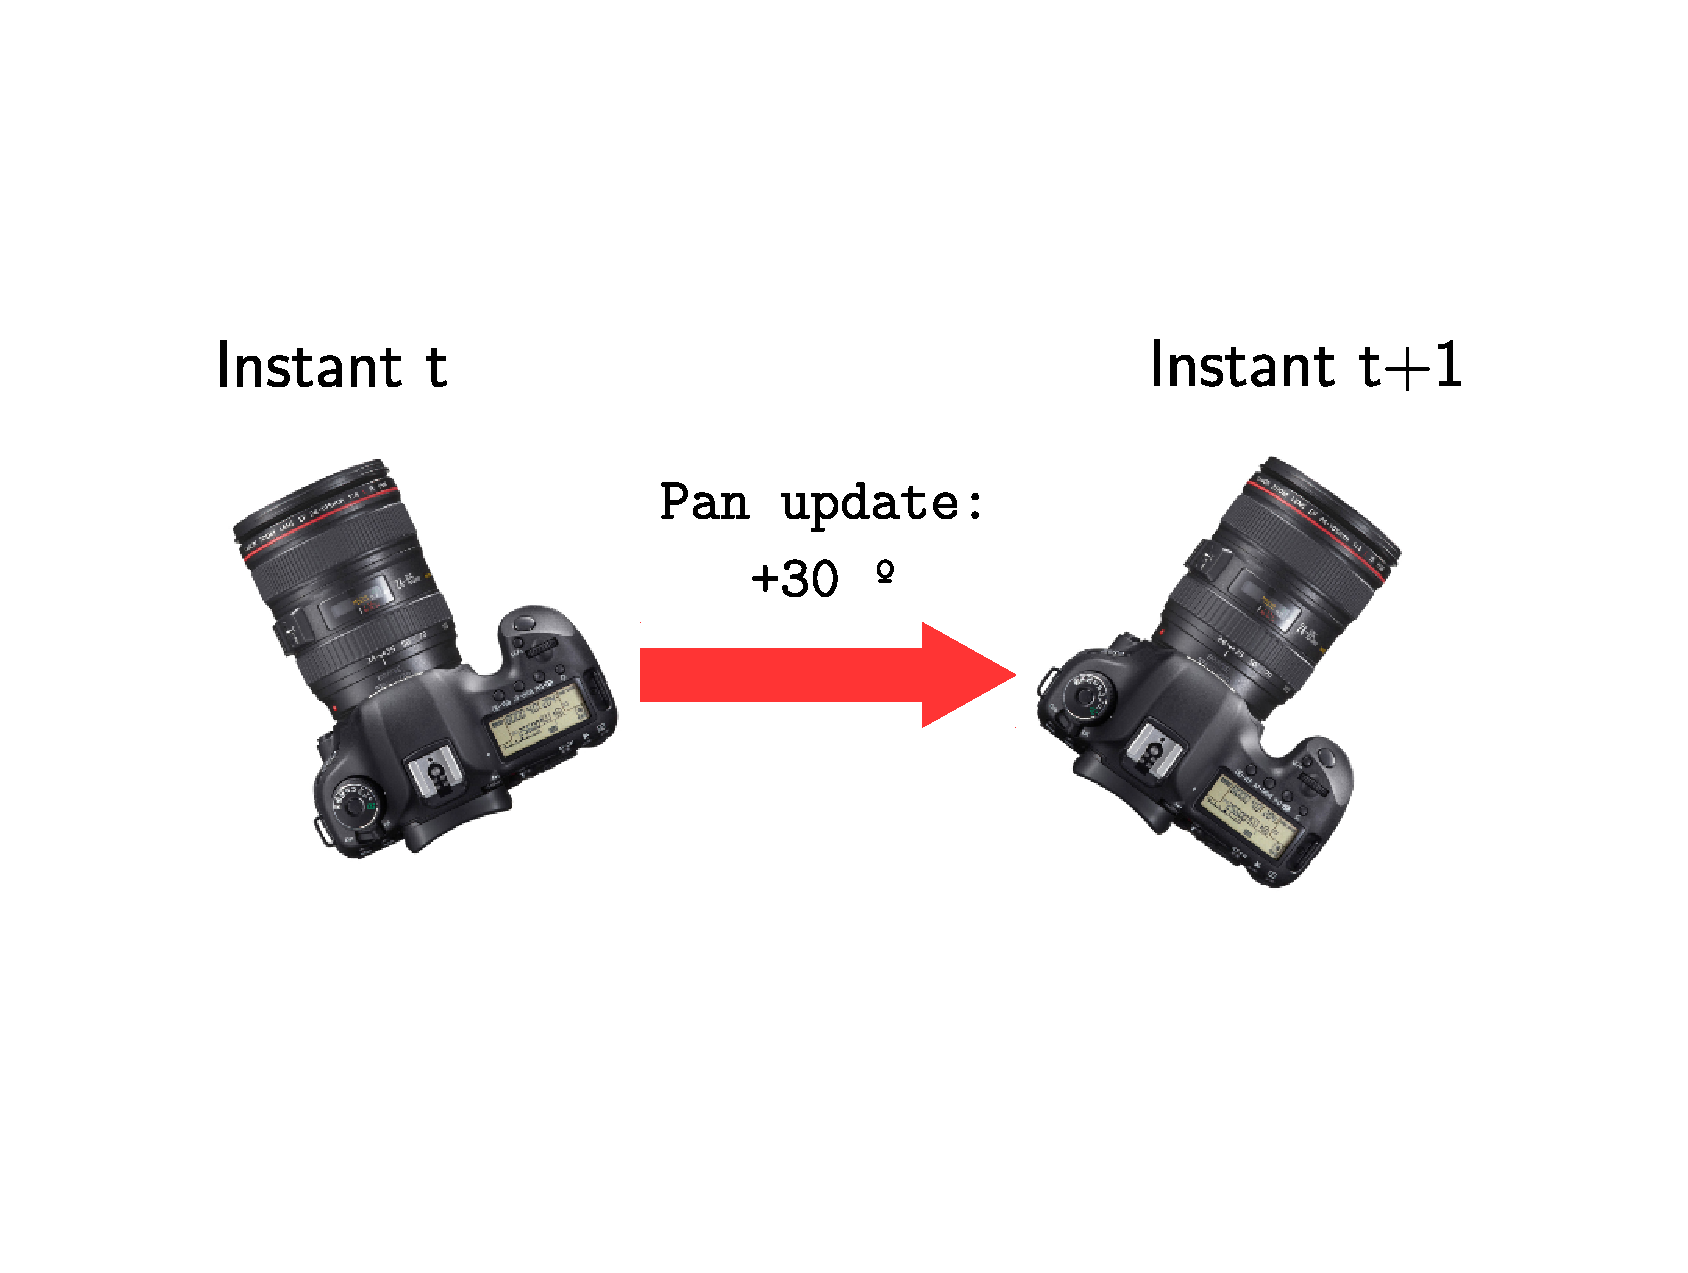
\includegraphics[width=2.7in]{images/ptz_wrong_movement}
				\caption{Wrong motion update (too long movements).}
				\label{fig:3_ptz_wrong}
			\end{subfigure}
			\qquad
			\begin{subfigure}[h]{0.4\linewidth}
				\centering
				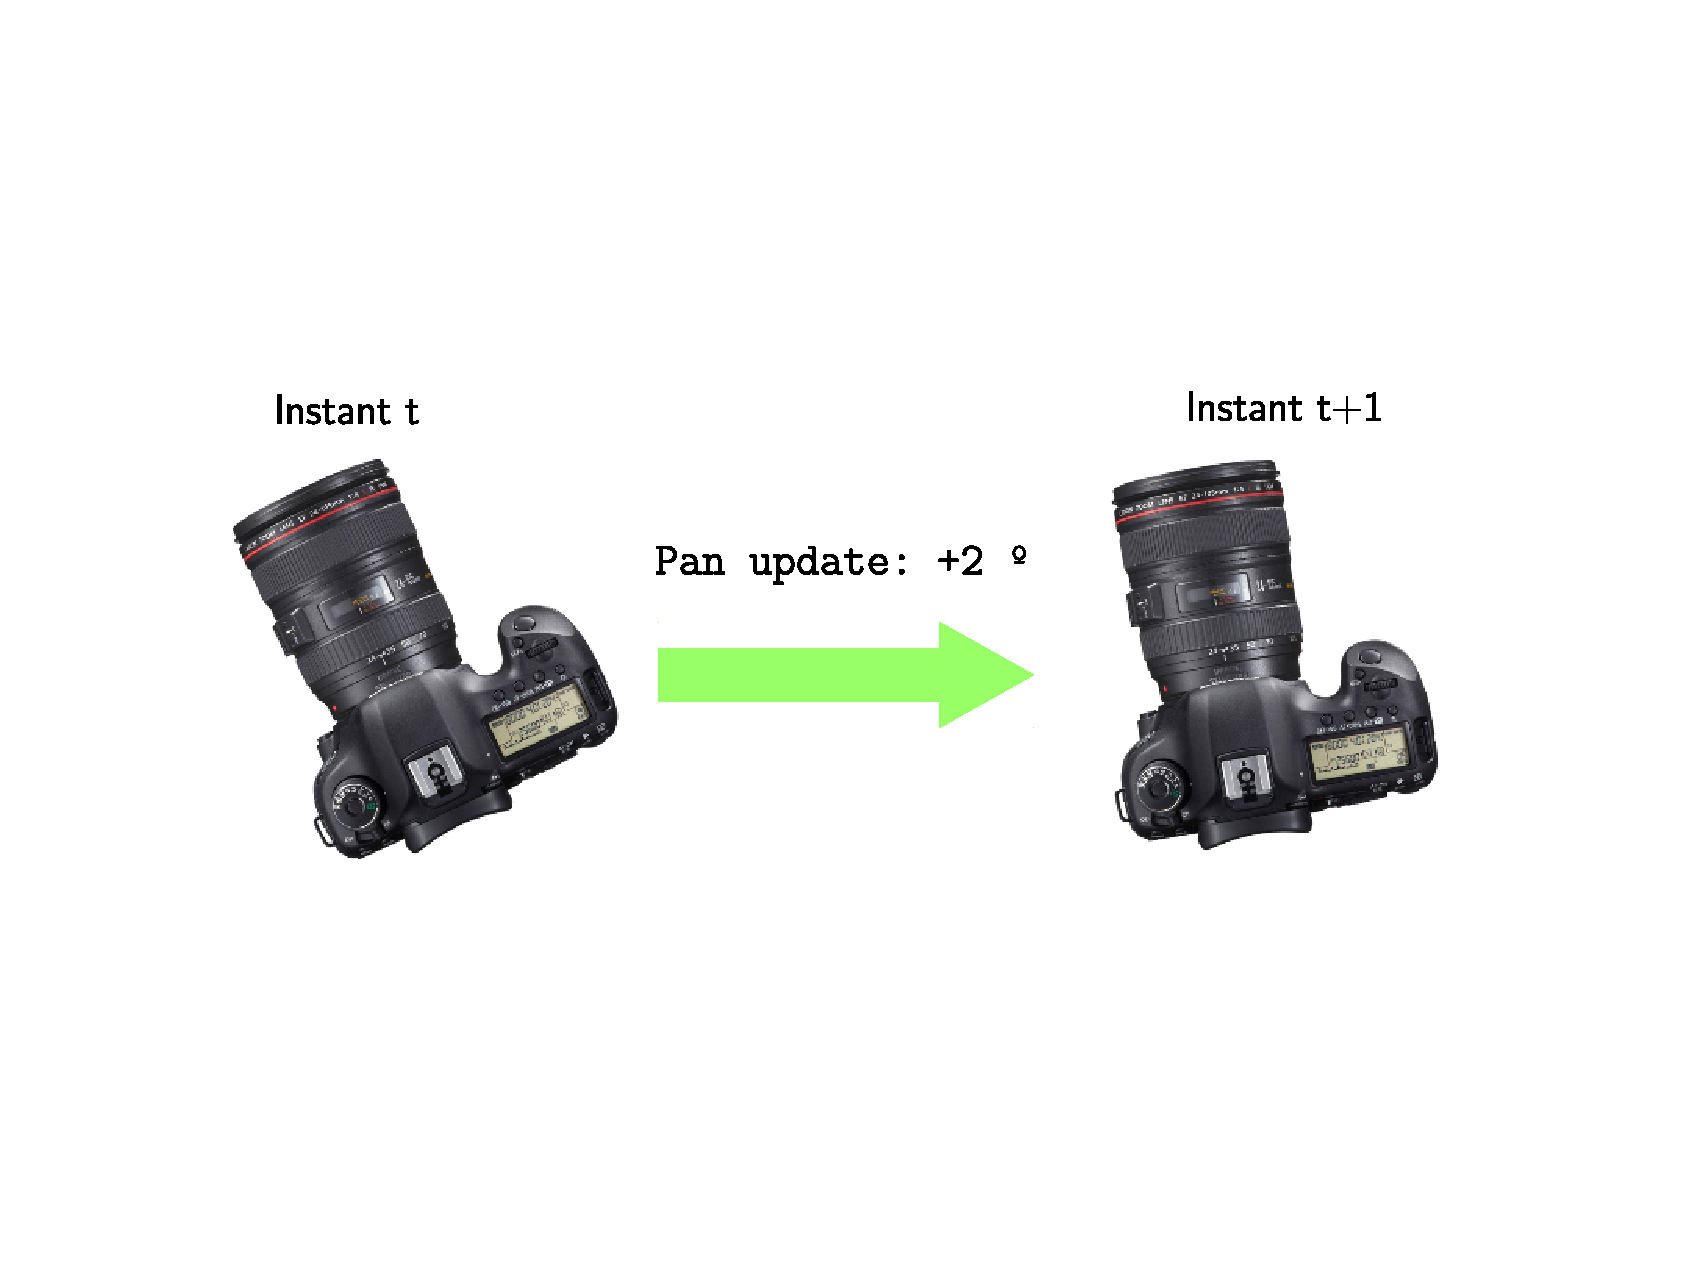
\includegraphics[width=2.7in]{images/ptz_correct_movement}
				\caption{Correct motion update (short differential movements).}
				\label{fig:3_ptz_right}
			\end{subfigure}
			\caption{Comparison between possible approaches for Pan/Tilt angle updates.}
			\label{fig:3_ptz_movements}
		\end{figure}
		

		This was the device we used for our first approximation to the sensing+actuating node (\autoref{sec:follow_ptz}), where the only response was moving the camera.\\

	\subsection{Asus Xtion Pro Live}
		It is a RGBD (RGB + Depth) sensor, designed by Asus for interactive PC applications development purposes. \\

		It has been our image source in the sensing+actuating node (\autoref{sec:follow_turtlebot}) we have developed. We used it in the second approximation (the response was the movement of the entire robot).

		\begin{figure}[h]
			\centering
			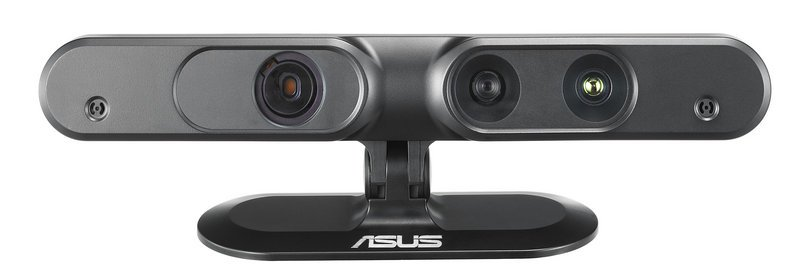
\includegraphics[width=0.4\linewidth]{images/xtion}
			\caption{Asus Xtion Pro Live. IR emitter (left), and RGB and IR lenses (right).}
			\label{fig:3_xtion}
		\end{figure}

		It counts on the left side with an IR (\emph{infrared}) light emitter, which radiates beams like a conventional light bulb (that's its function).\\

		On the right side, we can find two sensors:
		\begin{itemize}
			\item \emph{RGB sensor:} a conventional digital camera, with a resolution up to 1280x1024 px.
			
			\item \emph{Depth sensor:} it is capable of measure distance to objects, by receiving the reflections of the IR beams that we have mentioned above. It maps, for each pixel, the distance to that reflection (in mm), stored as a 16-bit long value.\\
			
			Thus, we can obtain a depth image, with a resolution of 640x480 px (@ 30 fps).
		\end{itemize}
		
		As it can be seen on \autoref{fig:3_xtion}, both sensor can't physically be in the same place, so there is a little discrepancy between both computed images:

		\begin{figure}[h]
			\centering
			\begin{subfigure}[h]{0.4\linewidth}
				\centering
				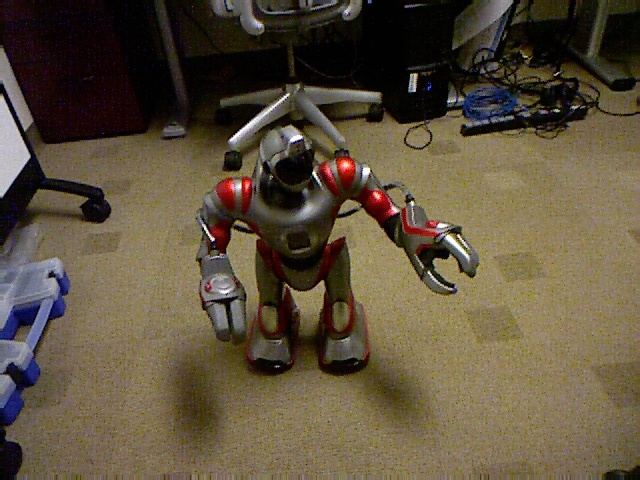
\includegraphics[width=3in]{images/rgb_before}
				\caption{RGB image.}
				\label{fig:3_rgb_bef_reg}
			\end{subfigure}
			\hfill
			\begin{subfigure}[h]{0.4\linewidth}
				\centering
				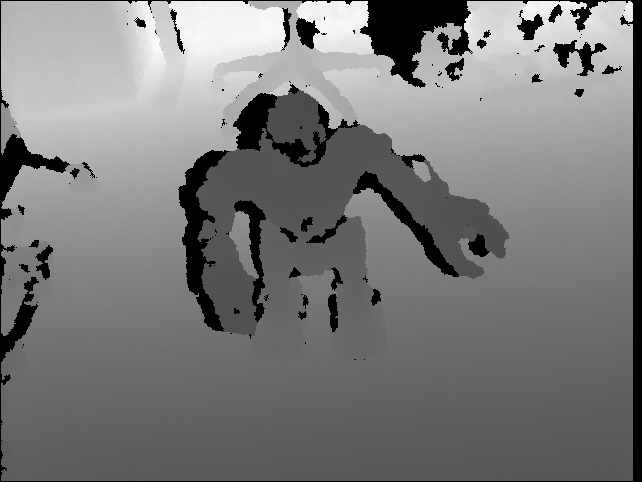
\includegraphics[width=3in]{images/depth_before}
				\caption{Depth image.}
				\label{fig:3_depth_bef_reg}
			\end{subfigure}
			
			\begin{subfigure}[h]{0.9\linewidth}
				\centering
				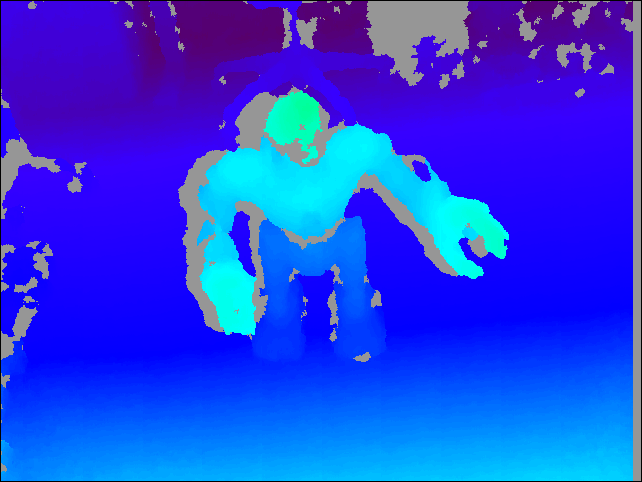
\includegraphics[width=3in]{images/disparity_before}
				\caption{Disparity (difference) between \ref{fig:3_rgb_bef_reg} and \ref{fig:3_depth_bef_reg}.}
				\label{fig:3_disparity_bef_reg}
			\end{subfigure}
			
			\caption{Both images sensed by the Xtion cameras, and the disparity between them \emph{before} the registration process.}
			\label{fig:3_bef_reg}
		\end{figure}
		
		With the goal of paliating this disparity, a process called \emph{registration} is executed for every new incoming depth image. It consists of a projection of the depth pixels into the RGB image, trying to align on an optimum way each pixel with its counterpart on the RGB image. We can observe that this can cancel to some degree the difference between both images (\autoref{fig:3_aft_reg}).
		
		
		\begin{figure}[h!]
			\centering
			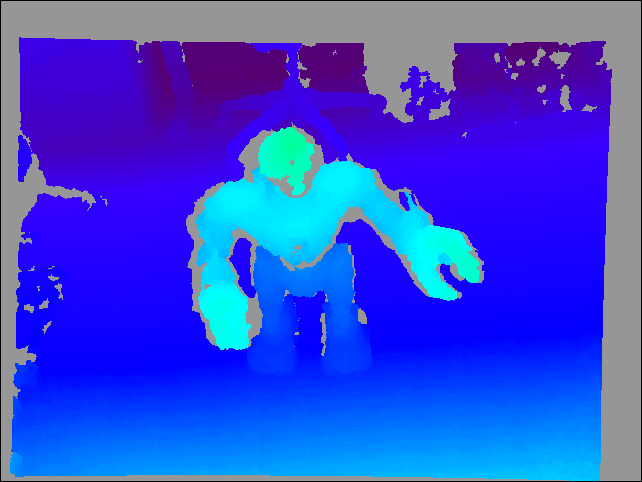
\includegraphics[width=3in]{images/disparity_after}
			\caption{Disparity between the images \emph{after} the registration process.}
			\label{fig:3_aft_reg}
		\end{figure}
		
		If we compare the new disparity (\autoref{fig:3_aft_reg}) with the previous disparity (\autoref{fig:3_disparity_bef_reg}), we can appreciate that now, the RGB and Depth images are aligned on an improved way, as if both sensors were on the same place, or much closer at least.\\
		
		So, from now on, we will call \emph{depth image} to the registered version of the depth map, as the unregistered image is not useful anymore.\\
		
		At last, we will make a mention to the open source drivers\footnote{\url{https://structure.io/openni}}, OpenNI (\emph{Open Natural Interaction}). They were originally developed by the Kinect developer company PrimeSense (which designed the Xtion device beside Asus).\\
		
		This interface allows to perform all the processes involved into handling this device (image grabbing, depth registration, etc.).
		
	\subsection{Turtlebot 2}
		The Turtlebot platform has been our main actuation platform on the developed actuation+response node (\autoref{chap:followperson}).\\
		
		\begin{figure}[h]
			\centering
			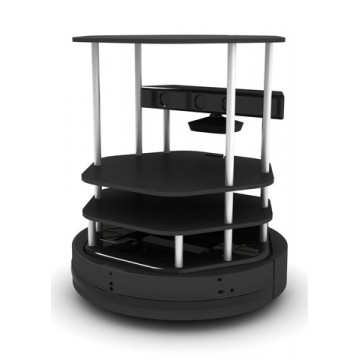
\includegraphics[width=3in]{images/turtlebot}
			\caption{Turtlebot development kit.}
			\label{fig:3_turtlebot}
		\end{figure}
		
		It is a research platform, composed by a structure jointed to a Kobuki robot (mobile base)\footnote{\url{http://kobuki.yujinrobot.com/about2/}}. Into this structure, there are also attached an Asus Xtion sensor (recently described), and a laser sensor, which has not been used on this project (nevertheless, it could be a continuation, as a navigation algorithm could be added to this project, on a similar way than in \cite{rocapal}).\\
	
		The user has the capability of connecting each of these devices via USB to the laptop, and place it at the top platform of the robot. From there, the computer can run the algorithm and command the movements. Every component can be handled with the respective ROS driver (which will be described later).
	

\section{Python}
	According to the official definition from \cite{python}, Python is \textit{an interpreted, object-oriented, high-level programming language with dynamic semantics}. It was created in 1991 by Guido van Rossum (who consecrated its name to the TV series \textit{Monty Python}). However, due to the increasing growth of \emph{Machine Learning} that happened the last two decades, it has become the most popular language for this purpose, due to its focus on \emph{easiness}, its duck typing\footnote{This refers to Python guessing about your variables, coming from the phrase \textit{''if it looks like a duck and sounds like a duck, chances are it's a duck."}} and its strong Object Orientation: everything can be treated as an object on this language. This is a very interesting feature, as it facilitates features as sharing memory, abstract processes, and much more.
	
	And, of course, it is \textit{Open Source}, so it is always under community improvements, and there are a vast number of incredibly useful third party libraries, which are impossibly easier to deploy onto your code.\\
	
	This makes this language a really potential candidate for the applications to develop (and that's precisely the reason that explains its huge growth on the software market).\\
	
	For our target, we will use Python on its version $2.7$. Although it is a relatively old version of the language, it is necessary to mantain the compatibility with ROS (\autoref{sec:3_ros}) bindings, which have not still taken the leap to the newest major version ($3.x$) on Python.\\
	
	Nevertheless, we want to mention the fact that Python is an \emph{interpreted} language, which means that its sentences are projected on another program (the Python interpreter, which executes them), and not directly by the processing hardware (CPU/GPU). This can be a con, as it makes the code execution much slower, in comparison with standard \emph{compiled} languages, which are run directly as processes, and taken by the computer hardware for its execution (as C, C++, Picky, etc.).

\section{ROS}
	\label{sec:3_ros}
	As it is said on \cite{ros-intro}, \emph{ROS} (Robot Operating System) is \textit{an open-source, meta-operating system for your robot}, maintained by the \emph{OSRF} (Open Source Robotics Foundation). It is a framework that provides a distributed, easily-scalable environment of \emph{nodes}. These nodes are programs which are independently running on the computer (or distributed over a P2P network), so they can perform individual tasks. However, they can communicate between themselves on a synchronous way (over \emph{services}, implementing a client-server role system between nodes), or on an asynchronous way, via \textbf{topics}, which will be the main benefit we will take advantage of. These topics, which rely on a standard TCP/UDP communication between sockets via the \texttt{loopback} interface, are intended for an unidirectional, streaming communication, where a node can take a role: \emph{publisher} (if it is writing data inside the topic), or \emph{subscriber} (if it is reading the data that publishers are broadcasting into the topic). The data flow through the topic, however, is not unrestricted. It must follow a ROS specific syntax, the \emph{Message} type, which is strictly defined for the communication purpose (geometry, sensoring, etc.).\\
	
	For our project we will be using the 2016 \textit{LTS} (Long Term Support) version, called \textit{Kinetic Kame}\footnote{\url{http://wiki.ros.org/kinetic}}. This is the version bundled on the installation of JdeRobot\footnote{\url{https://jderobot.org/Installation}}.\\
	
	ROS provides libraries and bindings for C++, Lisp, and \textit{Python} (\texttt{rospy}). They allow, among plenty of other stuff, to really easily set up a topic between two or more programs, which will be seen as ROS nodes.\\
	\begin{figure}[h]
		\begin{lstlisting}
...
import rospy
from std_msgs.msg import String
...
rospy.init_node('listener')              # Starting the node entity.
rospy.Subscriber('chatter', String)      # Instantiation of the topic subscriber.
rospy.spin()                             # 'Infinite loop' listening to the topic.
...
		\end{lstlisting}
		\caption{Simple stablishment of a listener node through \texttt{rospy} (code from \cite{listener-rospy}).}
		\label{fig:3_rospy_listener}
	\end{figure}
	
	However, this topic communication will be abstracted on our project by the \texttt{comm} library, as it will be seen on \autoref{sec:3_comm}.\\
	
	ROS also provides a Debian package, called \texttt{rosbash}, which allows to, in a very handy way, manage nodes and packages from a standard \texttt{bash} shell. The most remarkable feature for us is the command \texttt{roslaunch}, that launches a ROS node with a certain specific settings, configurable via a \texttt{.launch} file (which follows a XML formatting). An example for the file structure can be found on \autoref{fig:3_launch_file}.\\
	
	\subsection{\texttt{usb\_cam}}
	\label{sec:3_usb_cam}
		ROS node that creates a topic and publishes into it the digital video data incoming from a USB camera, into the topic \texttt{/usb\_cam/image\_raw}.\\
		
		This node will be used on the first approach to the sensing+actuating node (\autoref{sec:follow_ptz}), with the purpose of retrieving images from the Sony EVI D100P camera (\autoref{fig:3_evi}). In consequence, a custom configuration file\footnote{\url{https://github.com/RoboticsURJC-students/2017-tfg-nacho\_condes/blob/master/resources/usb\_cam-test.launch}} is required. We can have a glance on that configuration file (\autoref{fig:3_launch_file}).\\
		
		\begin{figure}[h]
			\centering
			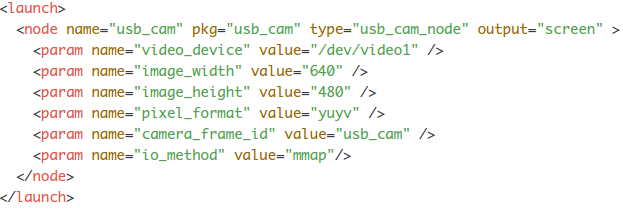
\includegraphics[width=5in]{images/usb_cam_test}
			\caption{Example of \texttt{usb\_cam-test.launch} configuration file for a ROS node.}
			\label{fig:3_launch_file}
		\end{figure}
		\begin{center}
			Usage: \texttt{roslaunch usb\_cam-test.launch}
		\end{center}

	\subsection{\texttt{openni2\_launch}}
		This ROS binding \cite{openni2-doc} provides the launch files for the \texttt{rgbd\_launch} node. This node publishes on several topics the RGB+D images provided by the Asus Xtion (\autoref{fig:3_xtion}), performing at the same time the registration process.\\
		
		This node will be used on the second iteration of the sensing+actuating node (\autoref{sec:follow_turtlebot}). It will connect the Xtion sensor to the component, providing the real-time imaging through the topic.\\

		\begin{center}
			Usage: \texttt{roslaunch openni2\_launch openni2.launch}
		\end{center}
		

	\subsection{\texttt{kobuki\_node}}
		This ROS package contains a bunch of launch files. Among them there is the one we will use: \texttt{minimal.launch}, which starts the \emph{nodelet}\footnote{A ROS nodelet performs multiple simultaneous processes, and consequently opens several topics.} that gives us the total control of the Kobuki robot connected to the computer\footnote{We refer to the robot as \emph{Kobuki} now because the mobile base of the Turtlebot (\autoref{fig:3_turtlebot}) is the only ROS device which we will control in our application.}.\\
		
		This node will be used on the second iteration of the sensing+actuating node (\autoref{sec:follow_turtlebot}). It will connect the Turtlebot motors to the component, providing the topic to command movements to them.
		
		\begin{center}
			Usage: \texttt{roslaunch kobuki\_node minimal.launch}
		\end{center}

	
\section{JdeRobot}
	As described in \autoref{sec:dl_jderobot}, JdeRobot\footnote{\url{https://jderobot.org}} is a distributed development platform/middleware, born in \cite{jmplaza-phd}. It stands out mainly for two key aspects:
	\begin{itemize}
		\item \textit{Hardware abstraction:} it behaves as an intermediate layer between control software (written by the programmer) and hardware, which can be a real device (a robot, drone, camera, laser scanner, etc.), or a simulation (on the open source world simulator Gazebo\footnote{\url{http://gazebosim.org/}}). This way, the bidirectional flow (information from sensors, and commands from the computer) is sent the same way, \textit{no matter the kind of the robotic device}.
		
		As well, this abstraction layer allows various computers to interact simultaneously with the hardware, as the communications are also abstracted to ROS topics or ICE endpoints (it will be properly explained at \autoref{sec:3_comm}), where a program has to just listen/talk to be in on. This provides a very valuable \textit{software and hardware scalability to the platform, and to the developed programs}.\\
		
		Let's have a look on a possible example on the \autoref{fig:3_jderobot_hal}. This could represent an scenario where somebody wants to virtually test a navigation algorithm. Thus, in the \emph{Computer 1}, a reactive controller is running, sensing the environment through a real laser scanner and a RGB camera (as in the work developed at \cite{rocapal}). This controller receives data from the sensors, computes a proper navigation response, and sends it to a virtual robot, simulated on Gazebo.
		
		Additionally, another machine (\emph{Computer 2}) is running a viewer, which allows it to draw the images seen by the camera, and the laser readings from the scanner. So, this component only receives the data from the sensors, and does not send any kind of data to the devices.
		
		We can see that both components can perfectly run together and on different machines, even when they are written over completely different languages (Python and C++, respectively). In addition, we can perfectly handle virtual and real devices simultaneously, even if they talk through different interfaces (ROS or ICE), due to the perfect support of this division by the \texttt{comm} (\autoref{sec:3_comm}) library.\\
		
		
		\begin{figure}[h!]
			\centering
			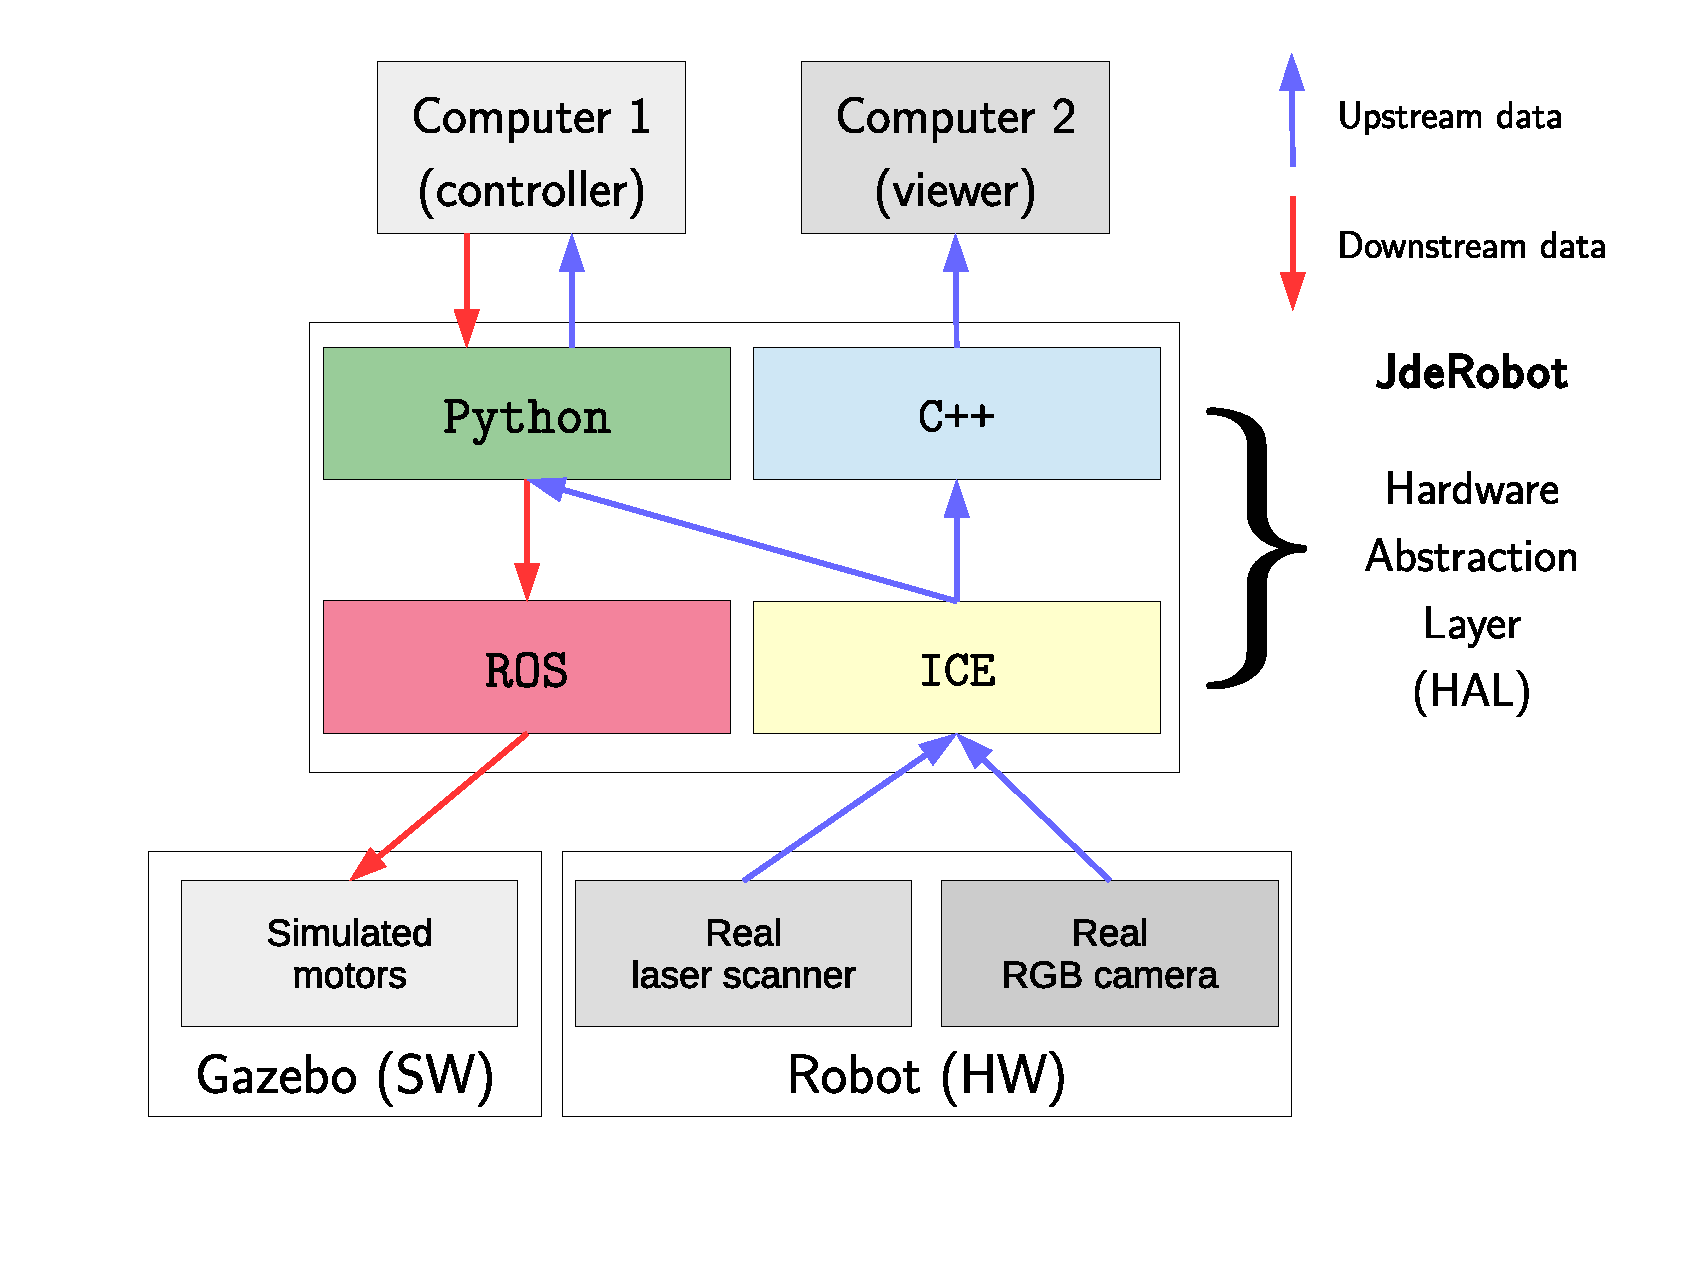
\includegraphics[width=4in]{images/jderobot_hal}
			\caption{JdeRobot abstraction layer, and a possible use distributed, multi-middleware scenario.}
			\label{fig:3_jderobot_hal}
		\end{figure}
		
		 \textit{So, in this easiness and flexibility resides the main advantage of using JdeRobot}.
		
		\item \textit{Wide device support:} JdeRobot provides full compatibility with ROS Kinetic Kame, so it can perfectly integrate with ROS Nodes (in our concern, we can communicate with the Turtlebot and the Xtion devices via several topics that the ROS intermediate nodes open).
		
		\item \textit{Behavioral based on threaded parallel schemes:} as it is introduced at  \cite{jmplaza-phd}, inside a component, we will find one or more \emph{schemes}, objectified on threads. These threads run concurrently with an specific timing (so it does not overload the CPU in vain if a few iterations per second are enough for a vivacious and correct response).\\
		
		These schemes perform different tasks each, as seen on \autoref{fig:2_tasks} on a non-blocking way, and share memory. This has been followed on a comfortable way on our implementation: the threads are independent, but the tasks they control are performed by Python objects, which are interconnected between them:
		
		As an example, we can see how this has been performed inside our Python code:
		
		\begin{figure}[h]
			\centering
			\begin{lstlisting}
...
cam = Camera(ros_topic)           # Creation of the camera.
net = Network(graph_model)        # Creation of the CNN.

net.setCamera(cam)                # Connection of the camera and the CNN,
                                  # which now can share memory.

t_cam = ThreadCamera(cam)         # Instantiation and start of the thread which
t_cam.start()                     # implements the Camera schema.

t_net = ThreadNetwork(net)        # Instantiation and start of the thread which
t_net.start()                     # implements the Network schema.
...
			\end{lstlisting}
			\caption{Handling schemes on Python with objects and threads.}
			\label{fig:3_schemes_python}
		\end{figure}
	\end{itemize}
	
	\vspace{0.4in}
	
	To sum up, we have described the goodness of the JdeRobot framework for our purposes, and seen how we can implement the \textit{useful schemes paradigm} on an easy way into Python, our development language.\\
	
	Now, in the next subsections, we will examine which of the JdeRobot components, apart of the structure, have been of greatest interest for us.
	
	\subsection{Digit Classifier}
	\label{sec:3_digitclassifier_jderobot}
		This JdeRobot component\footnote{\url{https://github.com/JdeRobot/dl-digitclassifier}} was originally designed by David Pascual \cite{dpascualhe} and Nuria Oyaga \cite{noyaga}, and it was used on this project to land on the concept of neural networks.\\
		
		Its design aims to \textit{classify handwritten numbers} with the use of a Convolutional Neural Network (\autoref{sec:1_cnn}), that classifies the incoming images from a video source.\\
		
		\begin{figure}[h]
			\centering
			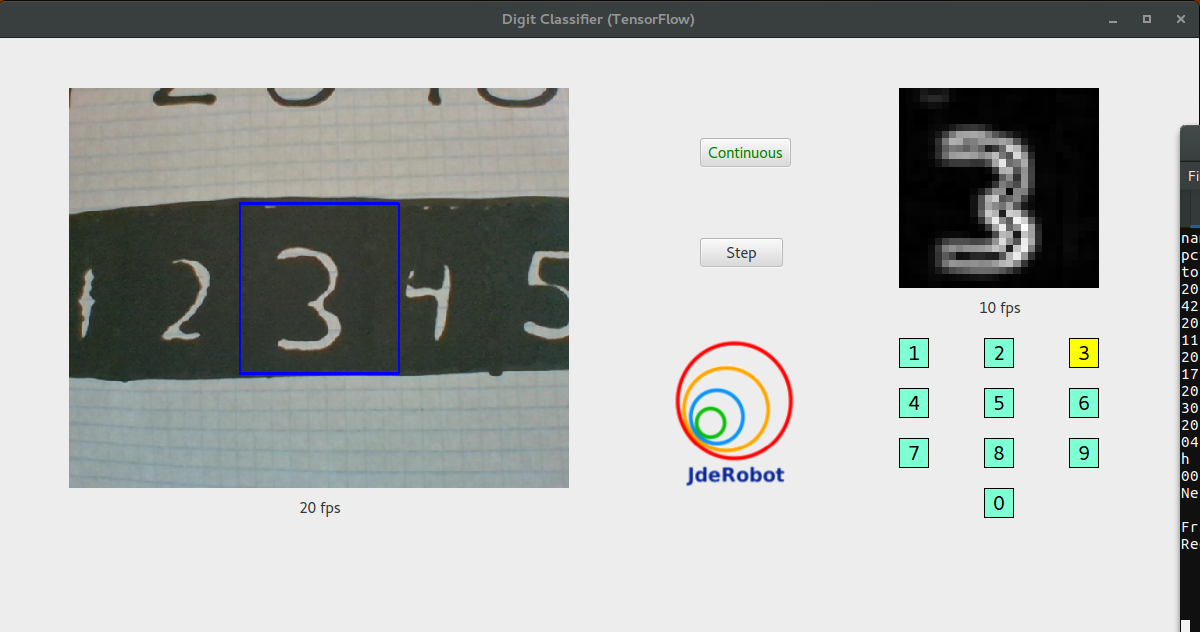
\includegraphics[width=4in]{images/digitclassifier}
			\caption{\texttt{DigitClassifier} on action.}
			\label{fig:3_digitclassifier}
		\end{figure}
		
		The previous implementations were written in Keras and Caffe (Python libraries to implement Neural Networks), so we made the same on TensorFlow (\autoref{sec:3_tensorflow}), to accomplish an initial domain of this Machine Learning framework.\\
		
		The implementation of this convolutional neural network consists on a concatenation of layers, following the scheme shown on \autoref{fig:3_digitclassifier_neural_structure}, which perform specific operations.
		
		\begin{figure}[h]
			\centering
			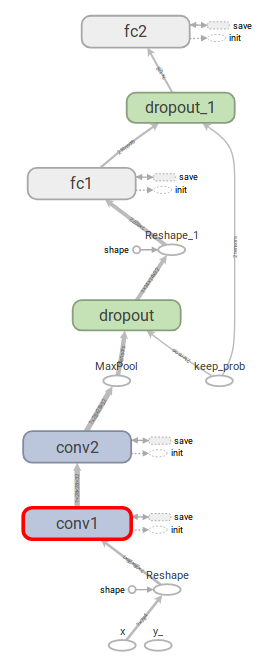
\includegraphics[width=2in]{images/digitclassifier_network_graph}
			\caption{Digit classifying neural structure.}
			\label{fig:3_digitclassifier_neural_structure}
		\end{figure}



		\begin{enumerate}
			\item \texttt{conv1}: first convolutional layer. As described in \autoref{sec:1_cnn}, it performs a 2D convolution between a $5px \times 5px$ square mask\/kernel (\texttt{W\_conv1}), and then adds a bias/intercept term (\texttt{b\_conv1}).\\
			\item \texttt{conv2}: second convolutional layer. It performs the same operation taking the output from the previous layer as an input, using a different weights mask and bias terms.\\
			
			Until now, what we have done is extracting patterns on each digit type (e.g. discovering typical circles on $0$ and $8$, which are always present on the same zone of the image).\\
			\item \texttt{pooling}: as the activation maps can be growing in size as we perform feed forward propagation, a \emph{pooling} operation is performed. It consists on sampling the input. Concretely, we retain the \textit{maximum} value for each 2 pixels, which is known as \textit{$2x2$ \texttt{max pooling}}
			
			\item \texttt{dropout}: this layer does not strictly perform any mathematical operations. It lets pass the TENSORS through it, but randomly switching off some neurons. This is parameterized by a user input, using a variable called \texttt{keep\_prob}. In our case, we set it to $0.5 (50\%)$ during the training process, to avoid overfitting by forcing the network to modify the neural paths randomly, as not every neuron is available on every moment. This is kind of similar to augmenting the dataset during the training process. The rest of the time (when the network is used to make inferences), this parameter is set to $1.0$, which means that no neurons are switched off at all.\\
			\item \texttt{fc1}: first fully connected layer. These layers, also known as \emph{dense} layers, are distinguised because every neuron is connected to every activation from the previous layer. So, this kind of layers are used for \text{pattern association with labels}, due to the relationship they can infer between every input.\\
			\item \texttt{fc2}: the output layer. It connects all the outputs of the previous dense layer and groups the output in a 10-dimensional vector, which contains the probability of the digit to belong to each one of the possible classes.
		\end{enumerate}


		
		Once all this was achieved, we upgraded the code (from single ICE support to ROS+ICE via the \texttt{comm} library), and unified it (Keras + TensorFlow frameworks in a single component, under choice using the YML configuration file) on the official JdeRobot repository. From there it can be used right out of the box with the included model for both frameworks. In addition, you can train your own models using the provided datasets, or yours if you build another.
	
	
	\subsection{\texttt{evicam\_driver}}
	\label{sec:3_evicam_driver}
	This driver, bundled into JdeRobot\footnote{\url{https://github.com/JdeRobot/JdeRobot/tree/master/src/drivers/evicam\_driver}}, allows the user to send movements commands to a Sony EVI D100P camera \autoref{fig:3_evi}) and retrieve information from it, creating an ICE endpoint that is ready to interact with the camera \emph{PT} (Pan, Tilt) motors.\\
	
	As this is a low-level driver, written in C++, it requires to be used on a specific way, which has been documented\footnote{\url{https://jderobot.org/Handbook\#PanTilt_Teleop}} to be easily applied in the future.\\
	
	This driver defines an interaction API with the camera, which allows us to get the values from the motors encoders:
	\begin{lstlisting}
import config
import comm
...

cfg = config.load('yml_configuration_file')
jdrc = comm.init(cfg, 'NodeName')


# Instantiation for the motors:
PTMotors = jdrc.getPTMotorsClient('NodeName.PTMotorsEndpoint')

print(PTMotors.getLimits()) # Shows the max/min values for pan, tilt 
                            # and each speed.

print(PTMotors.motors.data) # Shows the current values for pan, tilt
                            # and each speed.

# Let's move the camera! As easy as:
PTMotors.setPTMotorsData(new_pan, new_tilt, max_pan_speed, max_tilt_speed)
	\end{lstlisting}
	
	\subsection{\texttt{comm}}
		\label{sec:3_comm}
		\texttt{comm} is the basic library to perform communications between different components. It is what supports all the data flows in a typical scenario (\autoref{fig:3_jderobot_hal}).\\
		
		\texttt{comm} consists on a collection of bindings to easily create a link between two components, or between a device and a component. On the lowest level, we can use it relying on ROS (through topics as it was explained before on \autoref{sec:3_ros}), or through an ICE proxy. ICE\footnote{\url{https://zeroc.com/products/ice}} is an object-oriented middleware that, in our purpose, allows to abstract a data flow to a TCP/IP endpoint (an address/hostname, and a port), which can even support a communication between two or more programs inside the same machine.\\
		
		To create a communicator with \texttt{comm}, it needs the specification for that link (underlying middleware, topic/endpoint, etc.), so it uses the JdeRobot standard: YML\footnote{Legible data serialization format.} configuration files, which can be like in \autoref{fig:3_yml_format}.
		\begin{figure}[h]
			\centering
			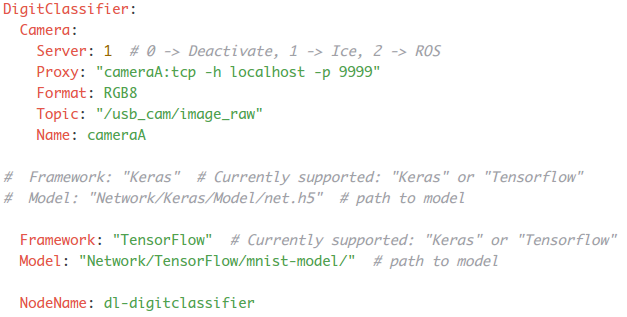
\includegraphics[width=4in]{images/yml_format}
			\caption{YML format on the \texttt{digitclassifier.yml} file.}
			\label{fig:3_yml_format}
		\end{figure}
		
\section{OpenCV}
\section{TensorFlow}
\label{sec:3_tensorflow}
\section{Keras}
\section{PyQt (v.5)}
\section{Threading}

	
	%%% DIGIT CLASSIFIER %%%
	\chapter{\texttt{DigitClassifier} node}
	\label{chap:4_digitclassifier}
	\section{Description}
		This JdeRobot component was originally designed by David Pascual \cite{dpascualhe} and Nuria Oyaga \cite{noyaga}, and it was used on this project to land on the concept of neural networks.\\
	
		Its design aims to \textit{classify handwritten numbers} with the use of a Convolutional Neural Network (\autoref{sec:1_cnn}), which classifies the incoming images from a video source.\\
		
		\begin{figure}[h]
			\centering
			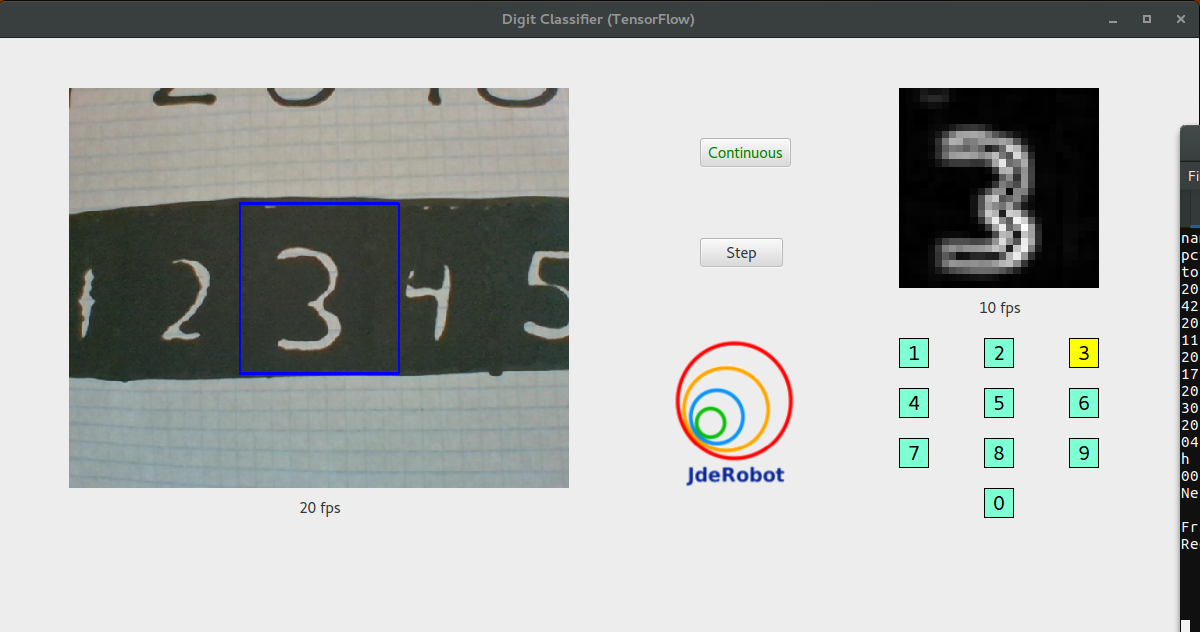
\includegraphics[width=4in]{images/digitclassifier}
			\caption{\texttt{DigitClassifier} on action.}
			\label{fig:4_digitclassifier}
		\end{figure}
		
		This kind of application (handwritten digits classification) is the typical first milestone to achieve in the domain of deep learning concepts and neural networks architectures, so lots of documentation are available online (a basic domain of the framework can be successfully achieved on the official TensorFlow tutorials\footnote{\url{https://www.tensorflow.org/tutorials/layers}} which, as said, teach how to deploy a handwritten digit classification system).\\


		As we mentioned, previous existing implementations were written in Keras \cite{dpascualhe} and Caffe \cite{noyaga} (Python libraries to implement Deep Learning algorithms), so we made the same on TensorFlow (\autoref{sec:3_tensorflow}), to accomplish an initial domain of this Machine Learning framework.\\
		
		After this, Keras and TensorFlow versions were merged on a single JdeRobot component: \texttt{dl-digitclassifier}\footnote{\url{https://github.com/JdeRobot/dl-digitclassifier}}, which has the scope to be functional on both libraries and, in addition, supports image streams from ICE endpoints or ROS topics (thanks to the \texttt{comm} library).\\
		
		As it can be seen it the \emph{README} file\footnote{\url{https://github.com/JdeRobot/dl-digitclassifier/blob/master/README.md}} in the repository, configuring the component is made pretty simple thanks to the YML file, so the reader is asked to feel encouraged to give it a try.\\
		
	\section{Functional infrastructure}
		As specified in \autoref{fig:2_tasks}, we divide the entire node functionality into individual tasks. These tasks have been implemented invoking a dedicated thread (using the \texttt{threading} library) for each one.\\
		
		\begin{figure}[h]
			\centering
			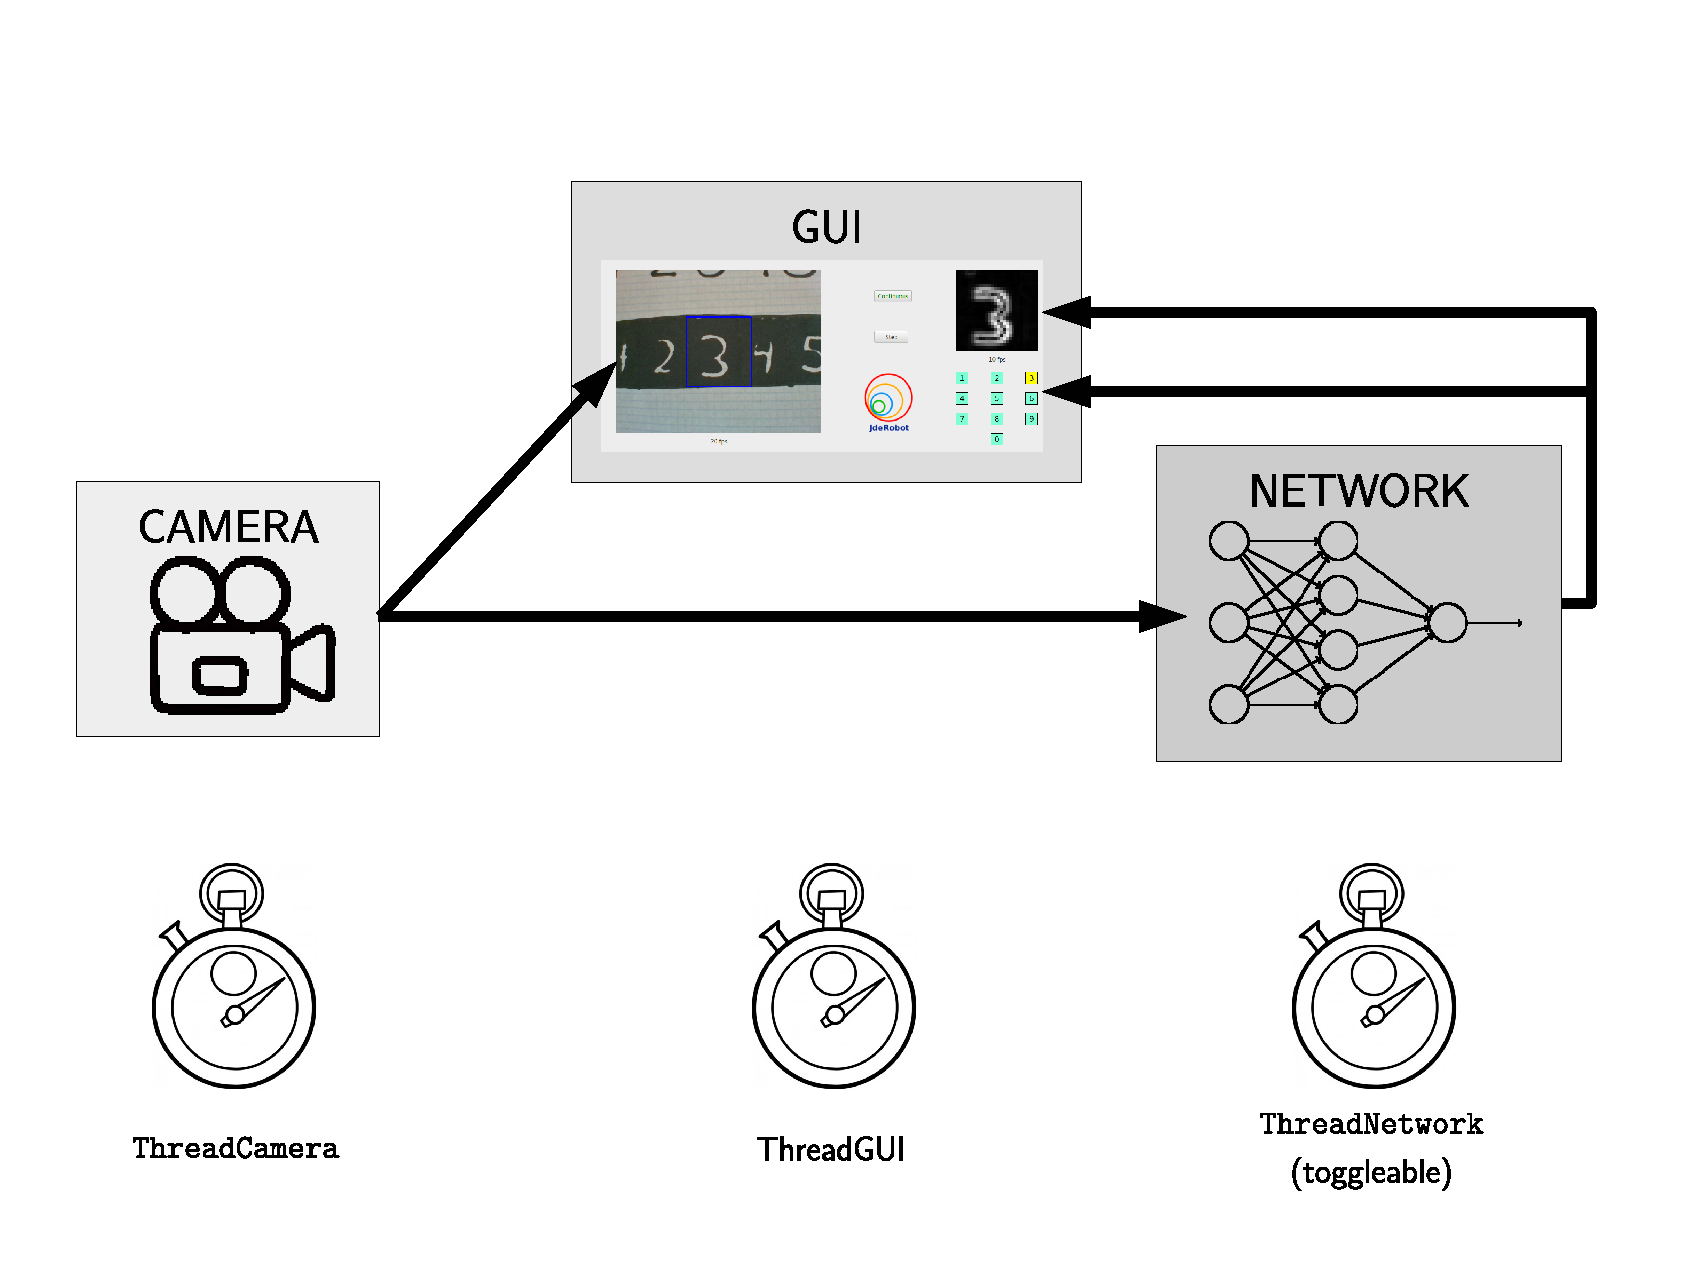
\includegraphics[width=5in]{images/digitclassifier_infrastructure}
			\caption{Infrastructure of the component (3 threads).}
			\label{fig:4_digitclassifier_infrastructure}
		\end{figure}
		
		
		
		This establishes the first functional difference with the previous version, which was powered by only 2 threads (for the camera and the GUI), performing on-demand (blocking) inferences on the neural network. Implementing a new thread dedicated to the neural network allows to have an instantaneous output digit from the network, ready to be grabbed on an easy and non-blocking way.\\
		
		Using the specified \texttt{threading} library, this deployment is as easy as:
		
		\begin{lstlisting}
import Camera, ThreadCamera
import GUI, ThreadGUI
import Network, ThreadNetwork
...


# We instantiate each object with its pertinent thread...
cam = Camera(cam_parameters)
t_cam = ThreadCamera(cam)

gui = GUI(gui_parameters)
t_gui = ThreadGUI(gui)

net = Network(net_parameters)
t_net = ThreadNetwork(net)

# Communicate them (according to the scheme)...
net.setCamera(cam)
gui.setCamera(cam)
gui.setNetwork(network)

# And start the application!
t_cam.start()
t_gui.start()
t_net.start()

gui.show()


		\end{lstlisting}
		Nevertheless, care has to be put on respecting parallelism between threads. This infrastructure is optimum for asynchronism, which means that one component does not depend on any others (e.g. the GUI component does not need the network to finish the next inference and return the classified digit in order to refresh the interface: it grabs the last inference made by the network \emph{from the own network}, which will be automatically updated when a newer one is available).
		
		This implies a respect to the independence between threads. It is the key for an asynchronous behavioral, as we want the component to yield the best possible performance.\\
		
	\section{Image processing}
		For every digit recognition system using a CNN, the approach is the same: \emph{processing a 28$\times$28 px image}\footnote{This particular shape is due to the used dataset, as it will be seen later.} containing a binary image of the digit itself. In addition to this, our system aims to a robust and correct classification at every feasible situation. Handwritten digits can often be found in visually harsh environments (poor quality sensor or lighting, trace indistinguishable of the background, etc.). Given this, before inserting an image on the network, we have to subject it to a \emph{preprocessing} pipeline:
		
		\begin{enumerate}
			\item Grab the central region of the incoming image from the camera (blue square on \autoref{fig:4_digitclassifier}).
			
			\item Convert the image to grayscale, as the color information is not relevant (hence, the network does not deal with RGB images, but just a grayscale 28$\times$28 matrix).
			
			\item Soften the image with a \emph{gaussian blur}, in order to reduce the possible noise on the image. We convolve the image with a square kernel of size 5 px.
			
			\item Resize the image to the necessary shape of 28$\times$28 pixels.
			
			\item Lastly, we \emph{extract the edges} of the image. This is not trivial, as the information we want to observe for the digits are the \emph{edges}. Otherwise, images on different contrast conditions would not be supported, as that would imply very different weights on the network for each situation. For this edge extraction, we apply a Sobel operator (which can be seen like computing the directional gradient/derivative in the image, as stated in \cite{sobel}) on each direction (vertical/horizontal), in order to detect the existing edges, and add them together in a single edge image, which is the final output of the pipeline.
		\end{enumerate}
		
		As a result, we obtain a softened shape map (even from different images, as seen on \autoref{fig:4_preprocessing}), which is a good start for the neural network to infer. This pipeline will be applied to every image (in the training process and while performing a new inference).
		
		\begin{figure}[h]
			\centering
			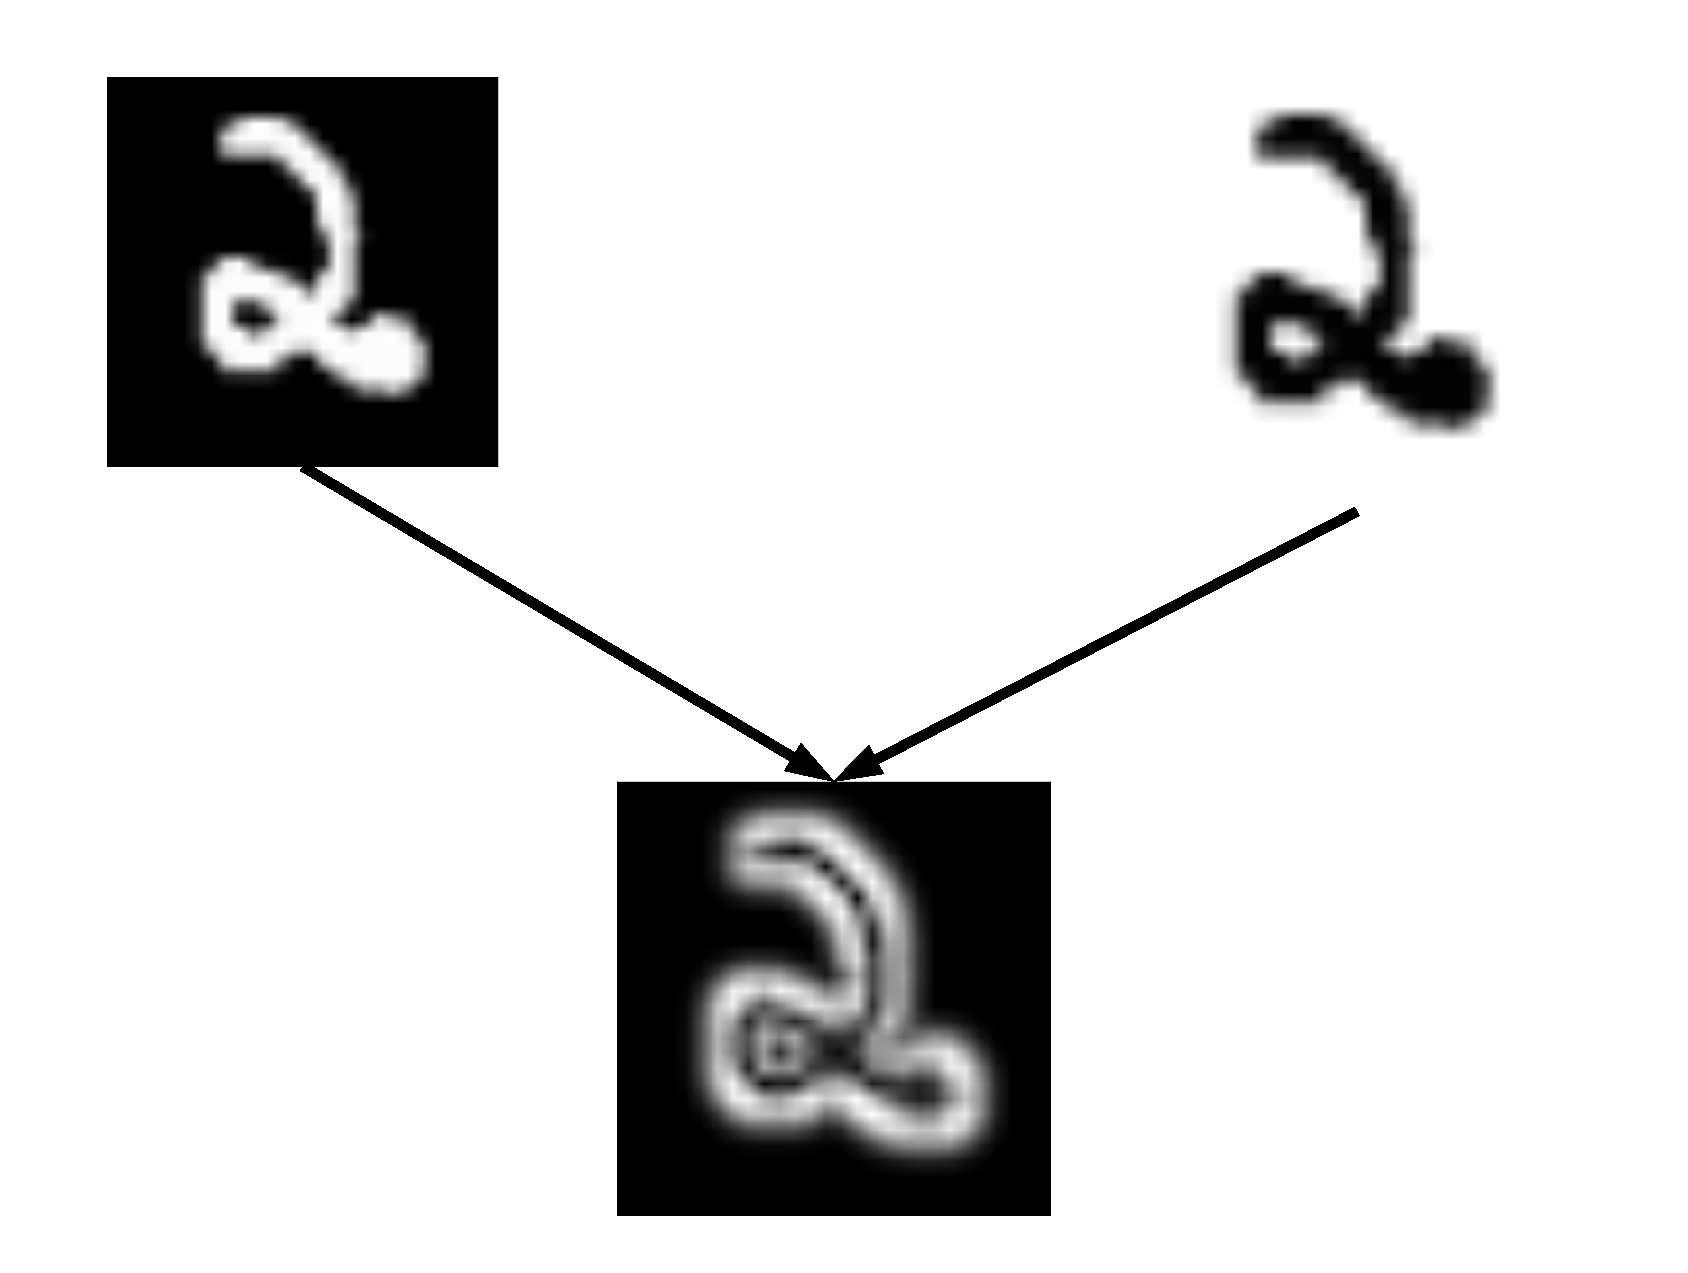
\includegraphics[width=5in]{images/digits_preprocessing}
			\caption{Result of the preprocessing (identical for both images).}
			\label{fig:4_preprocessing}
		\end{figure}

	\section{Digit classification CNN}

		The implementation of this convolutional neural network consists of a concatenation of layers, following the scheme shown on \autoref{fig:4_digitclassifier_neural_structure}. These layers are disposed in a serial structure, so the output of one layer (a vector containing what each neural activation function yields) acts as the input for the next one.
		
		For this reason, we need a first input layer, where all the pixels of the input image are mapped to a input neuron, on a bijective way.\\
		
		As stated before, the input shape for the images is 28$\times$28 px (a total of $28^2 = 784$ px), so we firstly perform a \emph{reshape} operation, which arranges the pixels on a 1-dimensional array of pixels. That will be the input for the network.
		
		\begin{figure}[h]
			\centering
			\begin{subfigure}[h]{0.65\linewidth}
				\centering
				
\includegraphics[width=4in]{images/mnist_net_example}
				\caption{High level layers visualization.}
			\end{subfigure}
			\begin{subfigure}[h]{0.3\linewidth}
				\centering
				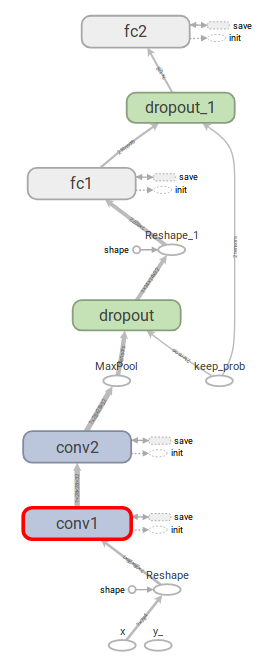
\includegraphics[width=1.7in]{images/digitclassifier_network_graph}
				\caption{Low level layers visualization.}
			\end{subfigure}
			\caption{Model of the implemented CNN for our system.}
			\label{fig:4_digitclassifier_neural_structure}
		\end{figure}
		
		\begin{enumerate}
			\item \texttt{conv1}: first convolutional layer. As described in \autoref{sec:1_cnn}, it performs a 2D convolution between a $5px \times 5px$ square mask/kernel (\texttt{W\_conv1}), and the image (which is seen again as a $28 \times 28$ matrix to perform the convolution). Later, the layer adds a bias/intercept term (\texttt{b\_conv1}). Thus, we obtain the activation for each neuron (the ReLU operator applied to the local convolution in the environment of that particular pixel), \texttt{h\_conv1}.
			
			\begin{lstlisting}
# Illustrative purposes.
# Some additional parameters (padding, stride) ignored.
h_conv1 = tf.nn.relu(tf.nn.conv2d(x, w_conv1) +  b_conv1)
			\end{lstlisting}
			
			To get a better understanding of what is happening here, we can have a glance of the weights learned on each neuron, for each digit (as we will study further below), on the \autoref{fig:4_activation_maps}.
			
			\begin{figure}[h]
				\centering
				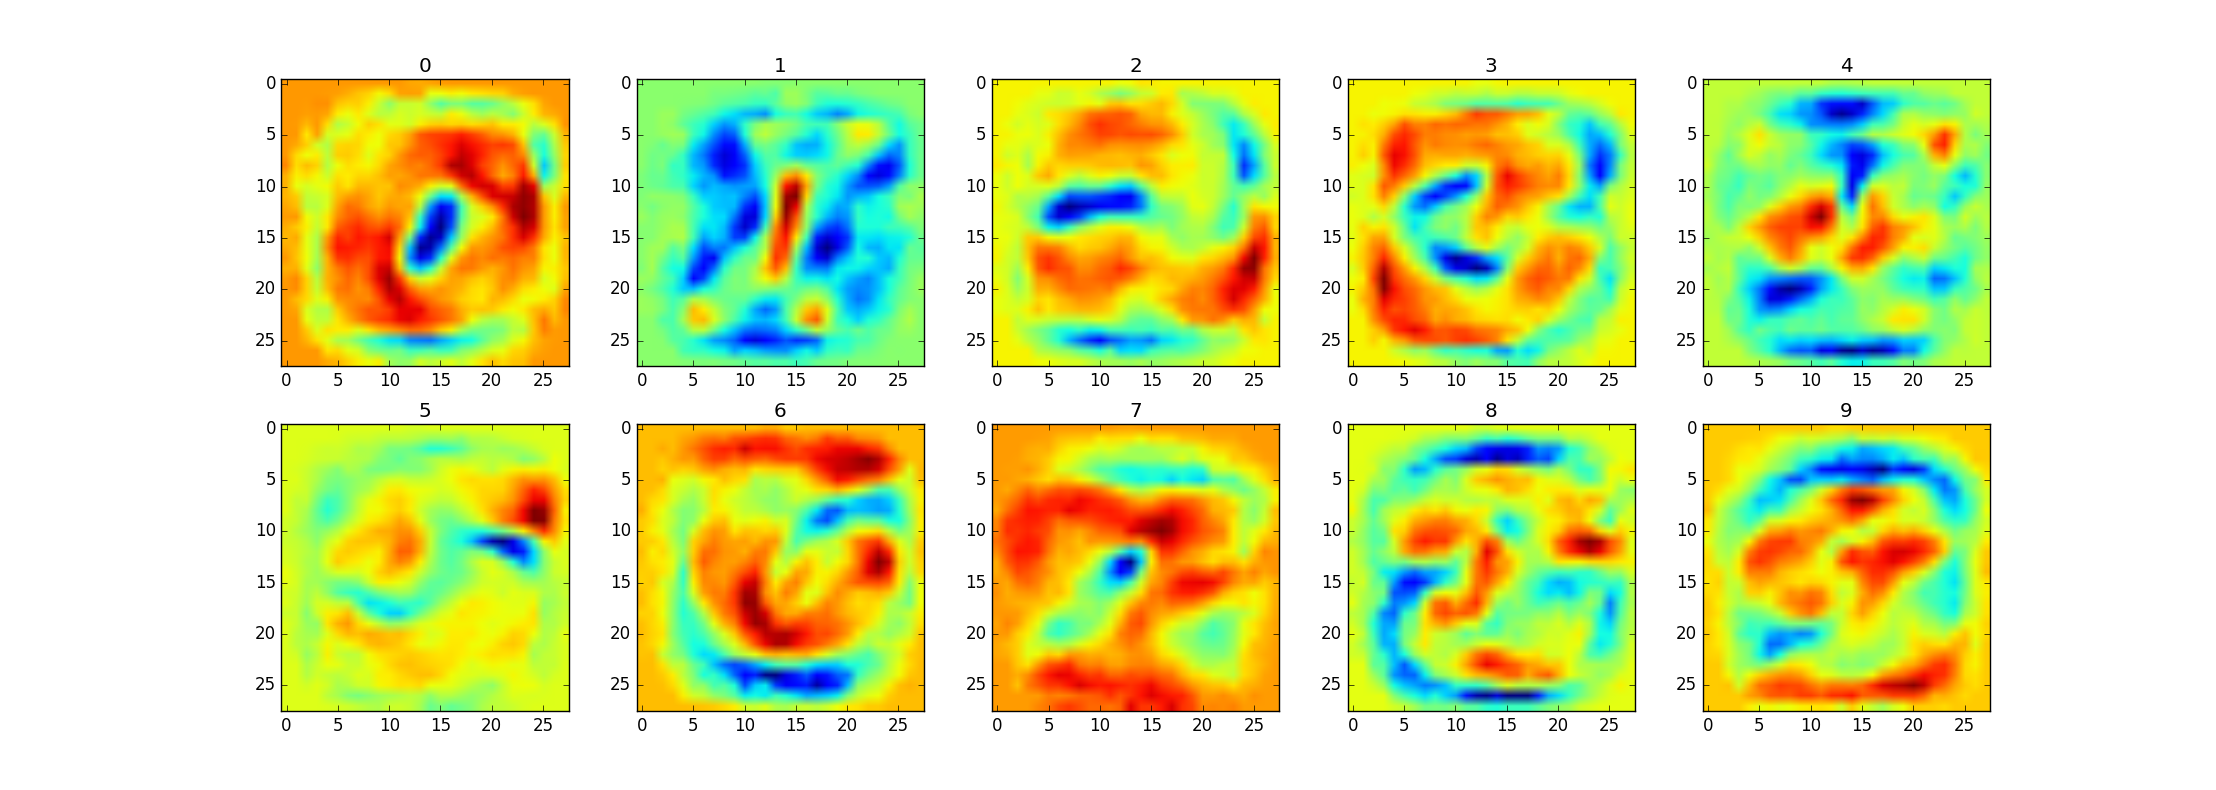
\includegraphics[width=6in]{images/digitclassifier_activation_maps}
				\caption{Heatmap for the learned weigths for each pixel and labeled digit.}
				\label{fig:4_activation_maps}
			\end{figure}
			
			This can begin to illustrate what is happening here: each neuron has a set of 10 tunable kernels, which depend on the value of what it has seen during the training process on its corresponding pixel and its environment. This illustration belongs to a simplified version of the network, where a convolution is not performed, but a simple \emph{matrix multiplication} (which can be seen as a convolution of kernel size equal to 1). So, we can see that the network is just learning where typically enabled pixels are situated on the input for each possible label ($0-9$).
			
			
			\item \texttt{conv2}: second convolutional layer. It performs the same operation taking the output from the previous layer as an input, using a different weights mask and bias terms.
			
			\begin{lstlisting}
h_conv2 = tf.nn.relu(tf.nn.conv2d(h_conv1, w_conv2) + b_conv2)
			\end{lstlisting}
			As we stated before, the tensor which will be convolved with the weights of this layer (\texttt{w\_conv2}) is now the output of the previous layer (\texttt{h\_conv1}).\\
			
			So far, what we have done is extracting patterns on each digit type (e.g. discovering typical circles on $0$ and $8$, which are always present on the same zone of the image).\\
			
			\item \texttt{pooling}: as the activation maps can be growing in size as we perform feed forward propagation, a \emph{pooling} operation is performed. It consists of spatially downsampling its input (the previous layer activation map). Concretely, we retain the \textit{maximum} value for each 2 pixels, which is known as \texttt{2x2 max pooling} (\autoref{fig:4_max_pooling}).
			
			\begin{figure}[h]
				\centering
				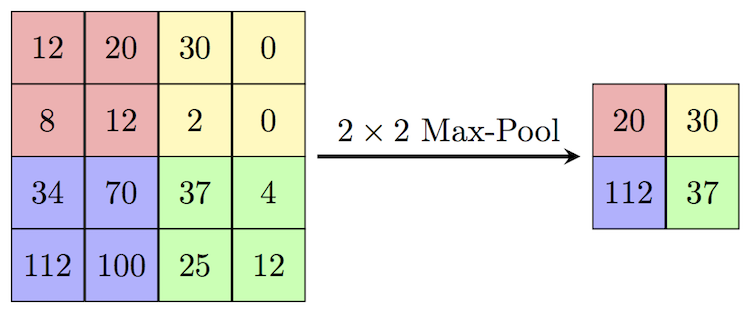
\includegraphics[width=4in]{images/max_pool}
				\caption{Max-pooling operation on a matrix.}
				\label{fig:4_max_pooling}
			\end{figure}
			
			\begin{lstlisting}
# Some additional parameters ignored here
# (kernel size, strides, padding).
h_pool = tf.nn.max_pool(h_conv2)
			\end{lstlisting}
			
			\item \texttt{dropout}: this layer does not strictly perform any mathematical operations. It lets pass the tensors through it, but randomly switching off some neurons. This is parameterized by a user input, using a variable called \texttt{keep\_prob} (which stands for the probability of a neuron staying switched on). In our case, we set it to $0.5 \ (50\%)$ during the training process, to avoid overfitting by forcing the network to modify the neural paths randomly, as not every neuron is available on every moment. This is kind of similar to augmenting the dataset during the training process. The rest of the time (when the network is used to make inferences), this parameter is set to $1.0 \ (100\%)$, which means that no neurons are switched off at all.\\
			
			\begin{lstlisting}
# The value for keep_prob is parameterized.
h_drop1 = tf.nn.dropout(h_pool, keep_prob)
			\end{lstlisting}
			
			
			\item \texttt{fc1}: first fully connected layer. So far, we have seen the pipeline as operable matrices. From now on, we go back to the \emph{single-dimension} activation map (array of outputs) model.
			
			These layers, also known as \emph{dense} layers, are distinguised because every neuron is connected to every activation from the previous layer. So, this kind of layers are used for \textit{pattern association with labels}, due to the relationship they can infer between every input.\\
			
			A thumb rule on this kind of layers is the more neurons included, the better generalization (the more correlation patterns we can detect between the activated zones on the incoming activation map). So, our implementation establishes a first dense layer of $14 \cdot 14 \cdot 32 = 6272$ neurons.\\
			
			\begin{lstlisting}
# Firstly, the last activation map is flattened into a 1 dimension array.
h_pool_flat = tf.reshape(h_drop1, [-1, 14*14*32])

# We model the full connection as a matricial multiplication
# (with a weight size of 14*14*32)
h_fc1 = tf.nn.relu(tf.matmul(h_pool_flat, w_fc1) + b_fc1)
			\end{lstlisting}
			
			\item \texttt{dropout}: to gain in strength, we deploy another dropout layer (which switches off random neurons with the same probability than the first dropout layer). This is remarkable, as we had performed a dropout process on the \textit{feature retrieval phase (first layers)}, but not on the \textit{pattern searching phase (dense layers)}.
			
			\begin{lstlisting}
h_drop2 = tf.nn.dropout(h_fc1, keep_prob)
			\end{lstlisting}		

			\item \texttt{fc2}: the output layer. It connects all the outputs of the previous dense layer and groups the output in a 10-dimensional vector, which contains the obtained \emph{logits}, a representative number for that class on the given image, which can be interpreted as a linear \emph{reward/tendence} \cite{sutton-barto} to belong to that class.
			
			As the last step, it applies a \textit{softmax} ($\sigma$) function to the output:
			\begin{equation}
				\sigma(z)_j = \frac{e^{z_j}}{\sum_{k=1}^{K}e^{z_k}}
			\end{equation}
			This function normalizes the output, mapping it between 0 and 1. This converts the mentioned raw numerical output into a \emph{probability} of being the given class (where the sum of the probability of all possible classes converges to $1$).
			
			\begin{lstlisting}
class_tendences = tf.nn.relu(tf.matmul(h_drop2, w_fc2) + b_fc2)

# Output (this is the called node to get the total inference output):
y = tf.nn.softmax(class_tendences)
			\end{lstlisting}
			
		\end{enumerate}
		
		This way, the total output of the CNN is a vector containing the probability of the image belonging to each class. If we keep the argument(s) of the maxima (\texttt{argmax}), we can find the most suitable class for that image.\\
		
		At this point, we can remember that the images entering into the network have been preprocessing, looking for the edges, so the learning process and the weights used through all the recently described pipeline can be generalized to all kind of images (as we will pass it previously through the Sobel edge detection filter).\\
			

		\subsection{Training the network}
			The reviewed pipeline is performed on an image, since it enters on the neural network until it goes out, passing through all the defined layers performing what is called \emph{feed-forward} propagation. However, the values of the activation maps and, hence, of the dense layer outputs (which determine the resulting class) depend on a relatively huge number of neurons, each one with its own weights and biases (for each class). As we can see, that is a ridiculous number of parameters to tune manually, hence we tune it automatically performing what is called \emph{backpropagation}.\\
			
			This backpropagation algorithm \cite{Rumelhart1986} performs a standard feedforward propagation (as described before) on what we call \emph{training set} (labeled images that will be used \emph{exclusively} for this purpose), which the system takes as examples which to learn of. Then, it compares the obtained output class ($argmax(softmax())$) for each input, and adjusts all the weights of the network, seeking to ensure that the difference between the \emph{desired} output (the \emph{ground truth} labels) and the \emph{obtained} result is minimum. This difference is computed and represented by a value which we call \emph{loss/cost} (the higher its value is, the worse, as there is a bigger difference between the correct and the obtained output).\\
			
			This tuning process is performed using what is called an \emph{optimizer}, which is an algorithm to search the optimum direction and magnitude update for every weight present on the network, depending on the obtained differences. As this can be such a complex process, it is performed on an \emph{iterative} way: evaluate a BATCH of training images, obtain the value for its loss, compute the suitable update values, and perform the weights update (scaled by what is called \emph{learning rate}, which determines the magnitude of the leap for each update). This way, after a number of iterations\footnote{This necessary number can not be determined, as it depends hugely on the dataset, purpose, network structure, learning parameters, etc. The best option is to monitor the loss/accuracy values during the training process, and stop it when these values converge (otherwise it could result in \emph{overfitting}, that is not convenient as it will only work fine on already seen examples).}, the model should converge to a global minimum for the loss function, which hopefully means that a suitable value for each weight has been found. This is the mechanism responsible of fitting the weights, so thank to it, we obtained, among many others, a reasonable values for the input layer on this network (\autoref{fig:4_activation_maps}).\\
			
			On our application, the chosen function to compute the lost value is the \emph{softmax cross-entropy} (as the name indicates, it is based on the \emph{softmax} version of the output, which means that it works with probabilities). It stands for the difference between the correct probability for a particular class (remember that each class is represented by a neural unit on the output layer: 1 if it's the suitable class, 0 otherwise), and the obtained output \emph{probability} \cite{cross-entropy}.
			
			This value is obtained on this way, being $y$ the binary correct output, and $p$ the computed softmaxed probability:\\
			
			\begin{equation}
				-(y \cdot log(p)) + (1-y) \cdot log(1-p)
			\end{equation}
		
			With respect to the optimization algorithm, the most intuitive option is the \emph{gradient descent algorithm} (that, in fact, is perfectly implementable on this system). Instead, we use the \emph{Adam} algorithm, which is an extension of the gradient descent approach. Its advantage is that it \emph{automatically adapts the learning rate} of the parameters adjustment, by computing its moving averages and variances (\emph{momentums}) \cite{adam-optimizer}. This is some more computationally expensive, but it is affordable. In exchange, we obtain an automatic training hyperparameters tuning, which is reflected in a faster and finer convergence to a correct value. It takes as input the cost function, and struggles to iteratively minimize it.\\
			
			
			Putting all this together, we can build these nodes on TensorFlow on an easy way, gearing the output (\texttt{y}) to the new optimization blocks:
			
			\begin{lstlisting}
# Cost function:
cross_entropy = tf.reduce_mean(
                  tf.nn.softmax_cross_entropy_with_logits_v2(labels=self.y_,
                                                                  logits=self.y))


# Optimizer (this is the called node during the training process):
train_step = tf.train.AdamOptimizer(1e-4).minimize(cross_entropy)

			\end{lstlisting}
		
		\subsection{MNIST dataset}
			\label{sec:4_mnist}
			MNIST (\emph{Modified National Institute of Standards and Technology database})\footnote{\url{http://yann.lecun.com/exdb/mnist/}} is a public database, which contains labeled binary images of handwritten digits. It is the result of jointing and shuffling\footnote{This is an important step to perform on databases, because we have to be sure of a correct \emph{generalization}: the data used for training must be of the same kind than for testing, to obtain fair results independently of the chosen dataset on each step.} two previous NIST's special databases (SD-1, containing digits written by Census Bureau employees, and SD-3, containing digits written by students), which were originally designed as training and test sets, respectively.\\
			
			All the included images respect the same format, with two key aspects:
			\begin{itemize}
				\item The images are \emph{square} $28 \times 28$ pixels matrices, containing the whole number (and anything else).
				
				\item The pixels represent binary values. This means that a pixel can only take values as \emph{digit} or as \emph{background}.
			\end{itemize}
			
			Given this, there are two image sets at our disposal: $60,000$ images for training, and $10,000$ images for testing\footnote{The \emph{test} set must not be used on the training process under any circumstance, to avoid unfair results, as this would be the equivalent to know an exam questions before taking it.}. Among all of them, we can obtain random examples (\autoref{fig:4_mnist_standard}).\\
			
			This is the image source we use to train our component, remembering that every image is preprocessed (\autoref{fig:4_preprocessing}) before going into the network.\\
			

		\subsection{Dataset augmentation}
			David \cite{dpascualhe} and Nuria \cite{noyaga} performed what is called a \emph{data augmentation} over the MNIST dataset, with the objective of \emph{pretend} to have a bigger number of samples to train.\\
			
			It consists of taking the existing images (on the standard MNIST dataset) and apply to it random (although controlled) transformations: each image suffers \emph{translations, rotations and zooms}, in addition to \emph{gaussian noise}. This has a double purpose: to \emph{get a bigger number of samples} (which is always a good thing), and to \emph{make a better model to process real world images}. As this network will classify real incoming digits from a camera, these digits will have most probably suffered noise (because of the camera and light conditions) and various geometrical transformations (as it can be shown to the camera with a slight tilt, or on a different background, etc.). Thus, we need to create a neural network which is ready to deal these harsh conditions. That is the main reason to augment the dataset performing these transformations.\\
			
			Taking all this on account, we have at our disposal the datasets they created\footnote{A link to download them for future usages is available on the \emph{README} file of the repository:\\ \url{https://github.com/JdeRobot/dl-digitclassifier}.}. As we can see on \autoref{fig:4_mnist_augmented}, this set of images is much harsher than the standard one (\autoref{fig:4_mnist_standard}). This will allow to create a much more robust model to classify real world digit images.\\



			\begin{figure}[h]
				\centering
				\begin{subfigure}[h]{0.45\linewidth}
					\centering
					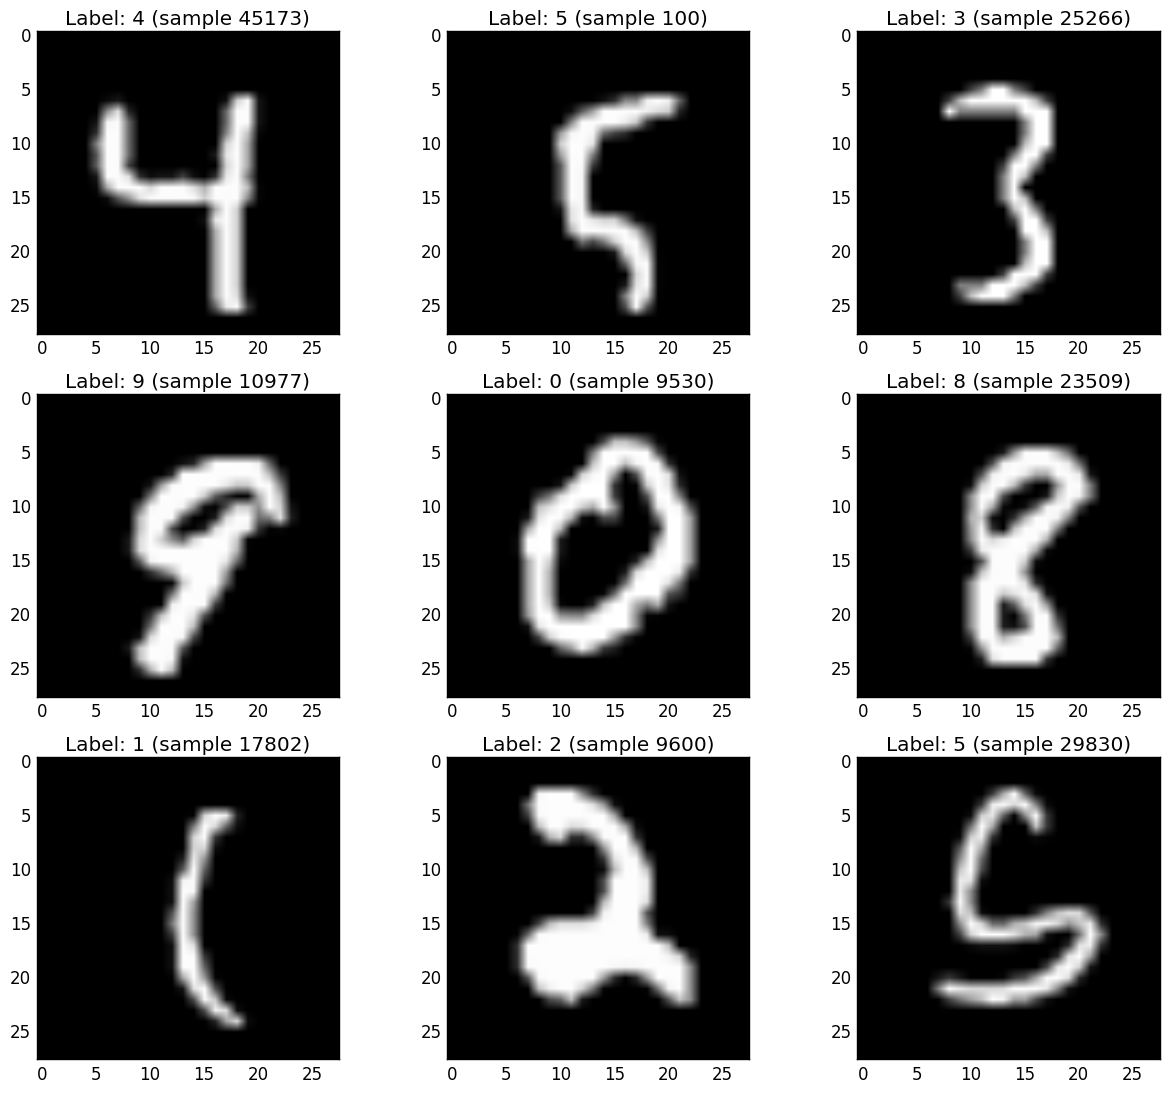
\includegraphics[width=2.7in]{images/training}
					\caption{Standard MNIST dataset.}
					\label{fig:4_mnist_standard}
				\end{subfigure}
				\qquad
				\begin{subfigure}[h]{0.45\linewidth}
					\centering
					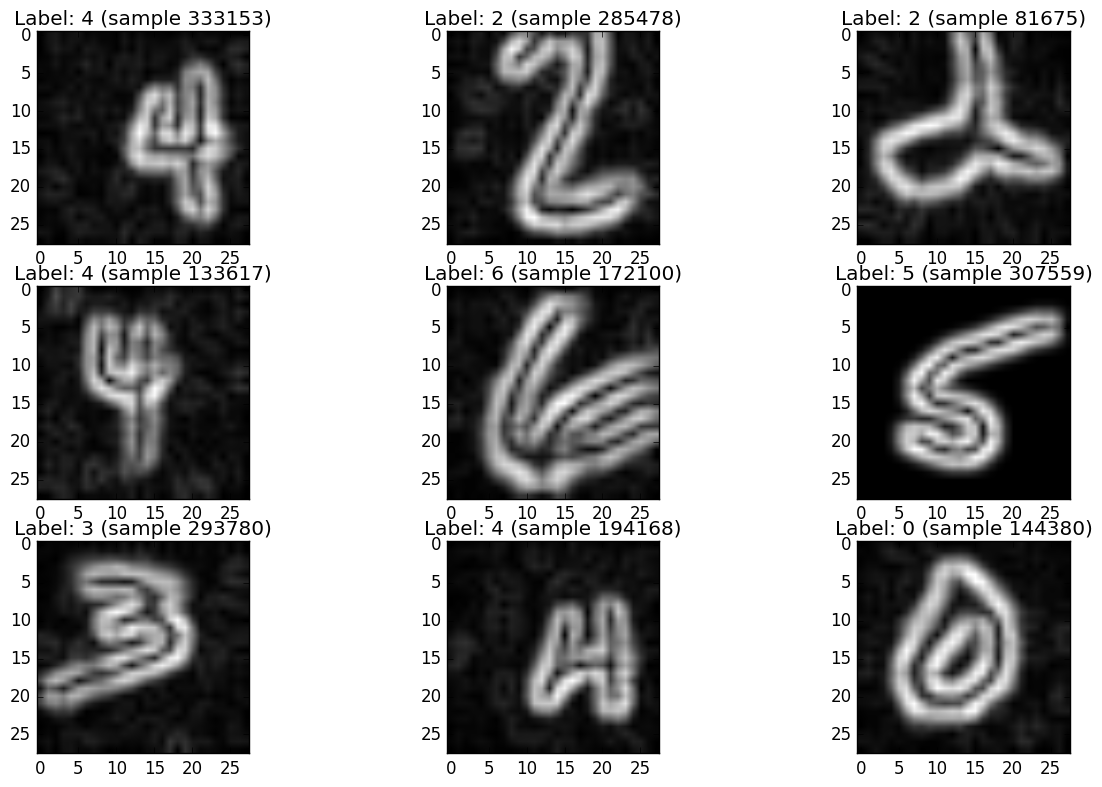
\includegraphics[width=3.5in]{images/training_augm}
					\caption{Augmented MNIST dataset.}
					\label{fig:4_mnist_augmented}
				\end{subfigure}
				\label{fig:4_mnist}
				\caption{Set of 9 random images extracted from the datasets.}
			\end{figure}


			These augmented datasets can be combined in different proportions (how many modified images are created for each standard image), which is typically indicated at its name: \texttt{training set x-y} means that there are \texttt{y} modified images for each \texttt{x} original one. To train the definitive model implemented on the classifier, we use the \texttt{1-6} model, which means that there are 6 modified versions of an image vs. 1 copy of the original one.


	
	%%%% OBJECT DETECTOR %%%
	\chapter{ObjectDetector tool}

\section{Description}
	Once we have some initial knowledge on CNNs applied to image processing, thank to the \texttt{DigitClassifier} component, we develop a new deep learning component, \texttt{ObjectDetector}\footnote{Demonstration videos available on the MediaWiki page (\url{https://jderobot.org/Naxvm-tfg}).}, which is capable of \emph{detect objects in a real-time image stream}\footnote{For a better compatibility with future usages for this component, it is able to process images from a local video/webcam directly using OpenCV (so \texttt{comm} is not required for the execution), specifying this in the YML configuration file.}.\\

	This component has a generic functionality, as the real-time processing capability is only used to display on the image where the objects are, wrapping them on what is called \emph{bounding boxes}. These boxes are the rectangles inside of which, theoretically the detected object is contained, and are delivered along the \emph{detection score}, and the corresponding \emph{class} detected. We will go further on this later.\\
	\begin{figure}[h]
		\centering
		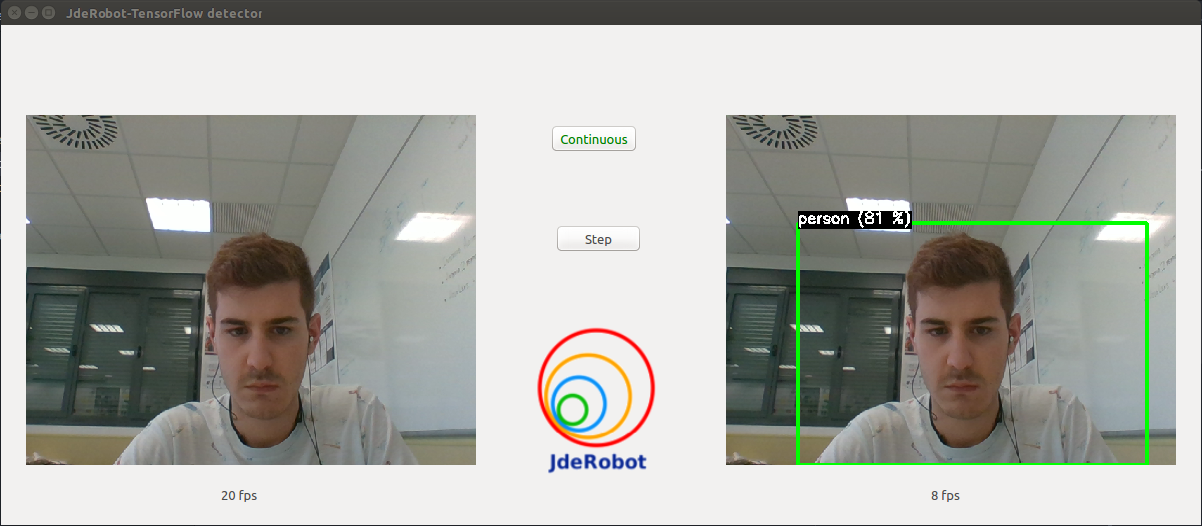
\includegraphics[width=4in]{images/objectdetector}
		\caption{\texttt{ObjectDetector} working.}
		\label{fig:5_objectdetector}
	\end{figure}
	
	We can notice that the type of problem that we are trying to solve now is different. Until now, we were trying to \emph{classify} images, based on a certain features that the network extracted by itself (the response always a classification, inferring an output even when no digit was shown to the camera, like shown on \autoref{fig:5_classifier_not_detecting}). Now, we are focused on \emph{detecting} objects inside an image. In other words, we want to distinguish whether an object (of a specific class or type) is present or not in the image that is being currently seen.
	
	\begin{figure}
		\centering
		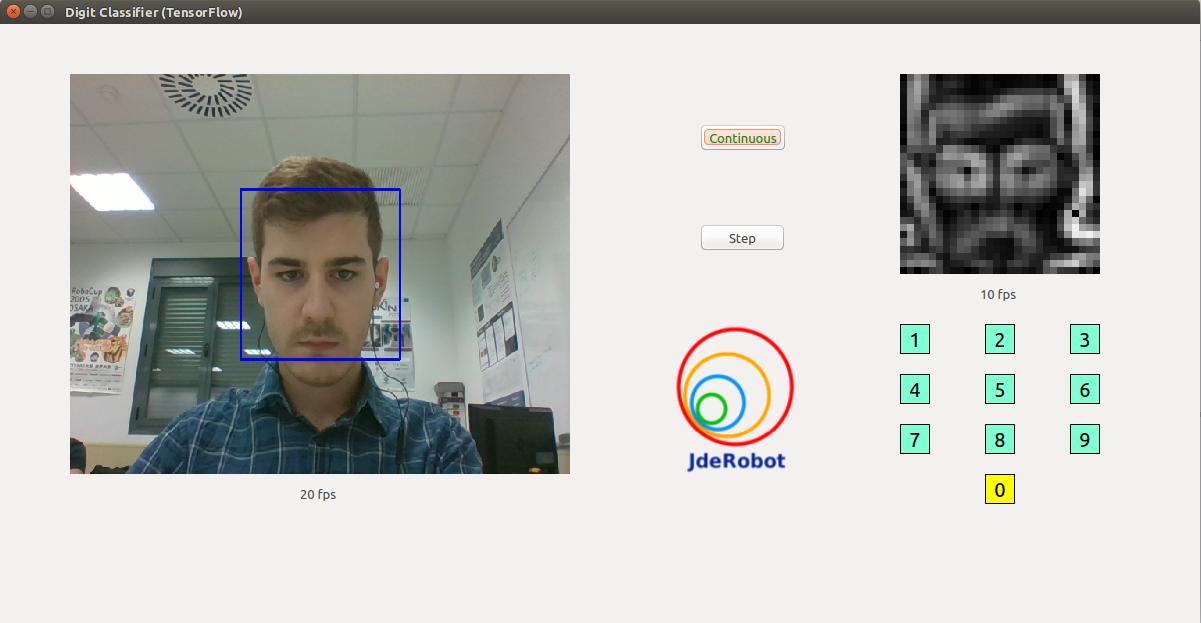
\includegraphics[width=4in]{images/digitclassifier_not_detection}
		\caption{\texttt{DigitClassifier}: a digit was always returned (or a subtle way of a computer to call you waste of space).}
		\label{fig:5_classifier_not_detecting}
	\end{figure}
	
	
	It should be mentioned that this purpose requires a much more complex CNN, which leads to a significantly heavier computational load on the machine (and, as a consequence, an importantly bigger inference time). Hence, a GPU-version of TensorFlow is highly recommended, as the CPU-version would take way too long for a real-time operation system.\\
	
	Due to this mentioned complexity, \emph{training a detection CNN} is out of the scope of this project (even so, with the proper resources, we could do it with some open-access labeled image datasets). Instead of this, we will pick some public models that the TensorFlow team has made available on the \emph{Detection Model Zoo}\footnote{\url{https://github.com/tensorflow/models/blob/master/research/object_detection/g3doc/detection_model_zoo.md}} (\autoref{fig:5_model_zoo}). On a parallel way, we have created a public mirror repository%
	\footnote{\url{http://jderobot.org/store/deeplearning-networks/}} inside JdeRobot containing some useful found models (for TensorFlow and Keras respectively).\\
	
	\begin{figure}[h]
		\centering
		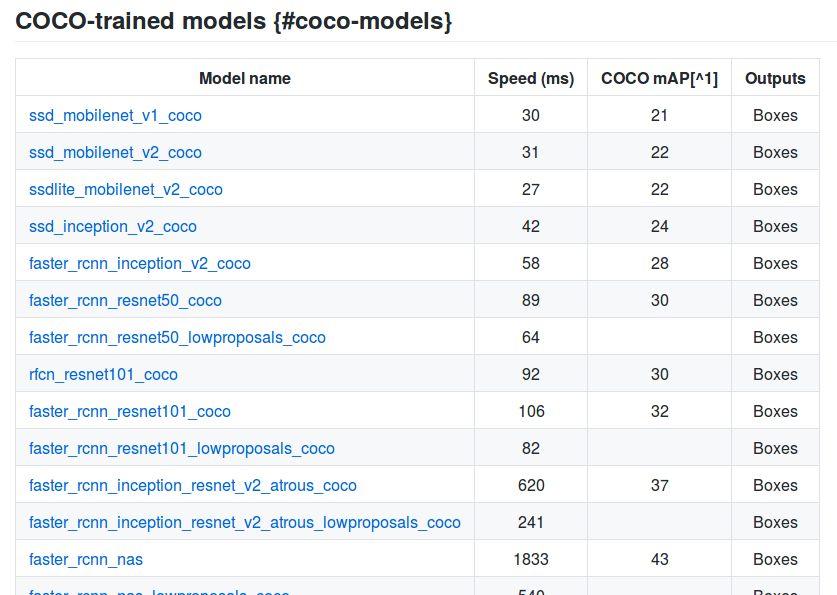
\includegraphics[width=4.5in]{images/detection_model_zoo}
		\caption{Some available models (July 2018) with their respective performance indicators.}
		\label{fig:5_model_zoo}
	\end{figure}
	
	
	These models have been trained on first-tier hardware, and are materialized in serialized files containing the graph structure and the corresponding weights for each neuron, on a ProtoBuf format (as we stated on \autoref{sec:3_tensorflow}). These model files are \textit{loadable at runtime} on a TensorFlow graph instance, so invoking one of these imported graphs is an easy task:
	\begin{figure}[h]
		\begin{lstlisting}
detection_graph = tf.Graph() # New graph instance.

# We use a context generator to set this graph as the default one
# on the TF backend:
with detection_graph.as_default():
	graph_def = tf.GraphDef()
	graph_def.ParseFromString(model_file)
	# We load this definition into the backend
	# (which contains the Graph instance).
	tf.import_graph_def(graph_def)
	
		\end{lstlisting}
		\caption{Generic model loading process.}
		\label{fig:5_load_model}
	\end{figure}

	
This way, we have successfully loaded the graph with its weights on the TensorFlow backend. The Python class (\texttt{DetectionNetwork}) we have defined allows to do this, choosing the desired model and dataset\footnote{Compatible with COCO, Kitti, OID and Pascal VOC datasets.} (we don't want the network to label a person as a dog) through the global YML configuration file.\\

Another thing to mention is the fact that, defining a \texttt{Writer} on the load process, we can inspect the graph structure on TensorBoard, as we will do later.

\section{Tool architecture}
	\label{sec:5_node_architecture}
	\begin{figure}[h]
		\centering
		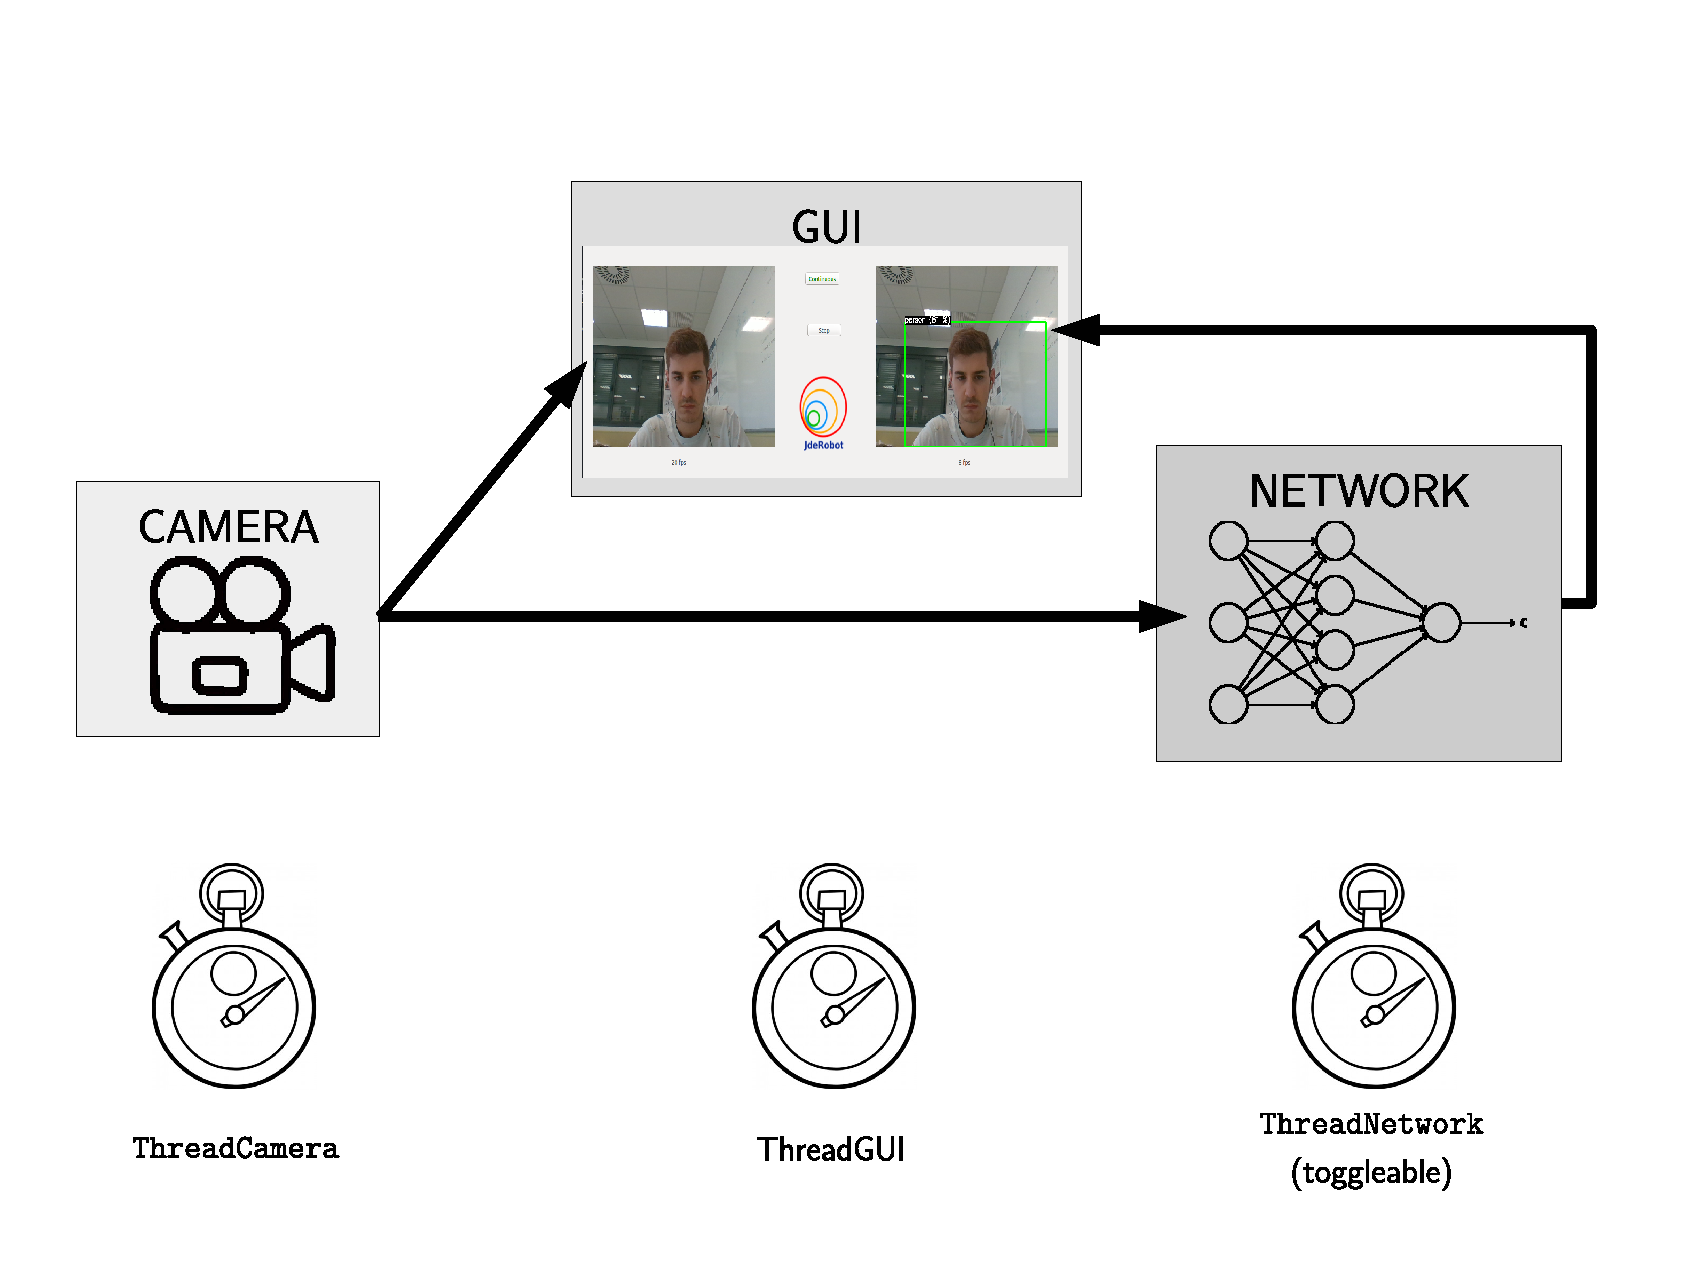
\includegraphics[width=4.5in]{images/objectdetector_infrastructure}
		\caption{Infrastructure of the component (3 threads).}
	\end{figure}
	
	This node inherits the architecture developed for the \emph{classification node}, consisting on 3 parallel threads. These threads drive the behavioral of separated objects, committed to perform independent tasks:
	\begin{itemize}
		\item \textit{Camera}: grabs the current image delivered by the communication framework (\texttt{comm} or OpenCV).
		
		\item \textit{GUI}: launches and updates the interface, with the fresh image from the camera. That image is drawn twice, as one of the representation (left) corresponds to the raw image from the camera, and the other one (right) is modified, including the bounding boxes, class and score for each detected object. This mentioned information is taken from the neural network. Hence, this component is connected respectively to the image source and the neural network.
		
		\item \textit{Network}: infers continuously the detected objects from the last received image, on an asynchronous way. When an inference is completed, the result (a set for each detection of bounding box, class and score for each single detection) is stored inside the \texttt{network} element. When the GUI needs the latest inference data, it just takes that data without any blocking call nor interrupting any process. This complies with the stated asynchronism requirement. 
	\end{itemize}
	
	Given this pretty identical structure to the \texttt{DigitClassifier} node, the schematic code to instantiate the program is the same than \texttt{DigitClassifier}'s (\autoref{fig:4_digitclassifier_code}).

	
\section{Detection CNN: SSD}
	As we have just mentioned, our application uses a SSD (\emph{Single Shot Multibox Detector}) CNN to perform the detection task. This choice has fundamentally taken based on the real-time performance expected from the component. We want it to make inferences as fast as possible (with a reasonable precision), so we chose this kind of architecture (it's more, it yields as good results as its slower counterparts).\\
	
	The high speed of inference of this kind of detectors is explained with the fact that \emph{it performs a single feed-forward pass} of the image through the network (on a \emph{single shot}, as it name states). According to its official release \cite{ssd-paper}, the rest of \emph{state-of-the-art} detection CNN technologies approach performing \emph{feature scaling} and \emph{bounding box proposals}. These techniques require more than one pass of the image or, at least, more than one single architecture, which rises the inference time.\\
	\subsection{Architecture}
		As we can observe in \autoref{fig:5_objectdetector_graph}, a \emph{SSD} detector has a defined network architecture, with some key aspects to keep its performance vs. inference time on the highest possible value. An inspection of the architecture using TensorBoard (\autoref{fig:5_objectdetector_graph}) reveals the pipeline structure, which is described below.
		
			
			\begin{figure}[h]
				\centering
				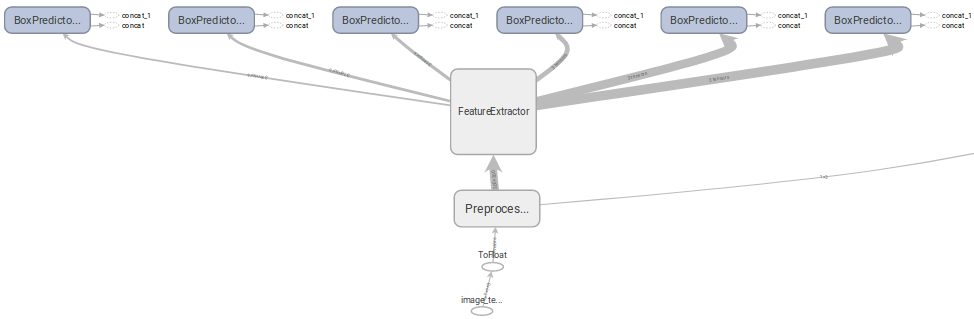
\includegraphics[width=\linewidth]{images/objectdetector_graph}
				\caption{SSD architecture on our model.}
				\label{fig:5_objectdetector_graph}
			\end{figure}
			

		\begin{enumerate}
			
			\item \emph{Preprocessing}: a first \emph{reshaping} stage is necessary due to the SSD operation. We can mention that this reshape is performed \emph{inside} the neural network, working directly with tensors on the GPU, which is probably faster than if we performed it with higher-level operations. This block reshapes the image to a 300$\times$300 size, which is the most typical image size on an SSD detector.
			\item \emph{Feature Extractor}: the architecture on a SSD CNN is based on a first group of layers (typically called the \emph{base network}), which deals with the \emph{feature extraction} part (as on the first stage of the classification network we designed on \autoref{sec:4_classif_cnn}). This particular model has a \emph{MobileNet} based feature extraction network\footnote{\emph{MobileNets} are originally designed to embed \emph{small, low latency} deep learning systems on low-spec devices \cite{mobilenet}, squeezing the trade-off between performance and inference time. So, we can reuse that part of its architecture for our proposal.}.  As it is formed by a concatenation of convolutional layers (\autoref{fig:5_mobilenet}), the resulting \emph{feature maps} will be gradually smaller and deeper while we go forward. These maps sets will be convolved with the original image, so the smaller the activation map is, the bigger its \emph{receptive field} will be (hence, it will useful to detect bigger objects). Given this, we are capable of \emph{extract} 6 intermediate sets (described on \autoref{tab:5_sets_imagenet}), with the objective of \emph{detect objects of different sizes}.
			
			\begin{figure}[h]
				\centering
				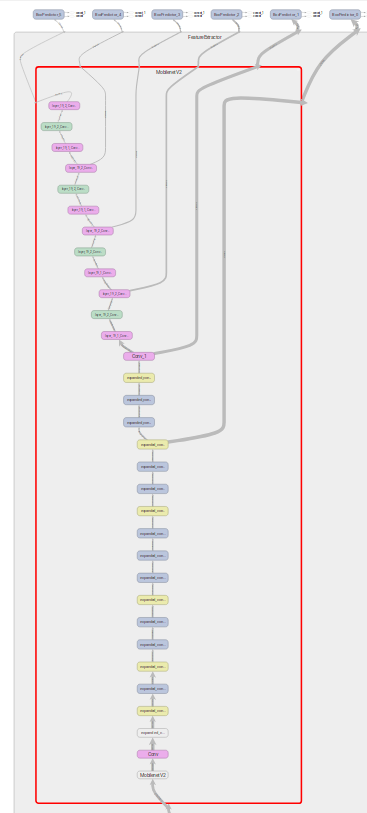
\includegraphics[width=2in]{images/ssd_mobilenet_2}
				\caption{\emph{MobileNet} pipeline.}
				\label{fig:5_mobilenet}
			\end{figure}

			\begin{table}[h]
				\centering
				\begin{tabular}{|c|c|c|}\hline
					\textbf{\# Set} & \textbf{Shape} & \textbf{Depth} \\ \hline
					1              & 1$\times$1     & 128            \\
					2              & 2$\times$2     & 256            \\
					3              & 3$\times$3     & 256            \\
					4              & 5$\times$5     & 512            \\
					5              & 10$\times$10   & 1280           \\
					6              & 19$\times$19   & 576           \\ \hline
				\end{tabular}
				\caption{Description of the 6 extracted feature maps sets on our implementation.}
				\label{tab:5_sets_imagenet}
			\end{table}
	
			
			\item \emph{Box Predictors}: later, for each extracted set, a dedicated operation is performed (that's the reason why we have 6 identical boxes on the TensorBoard analysis (\autoref{fig:5_objectdetector_graph}). They will perform the same operation but in patches of different sizes/depths, to detect \emph{objects on different scales}). Into this component, for each layer of the extracted feature set, a small set (3-4 typically) of bounding boxes (called \emph{priors}) with different \emph{aspect ratios} are generated (\autoref{fig:5_ssd_generated_boxes}).
			
			\begin{figure}[h]
				\centering
				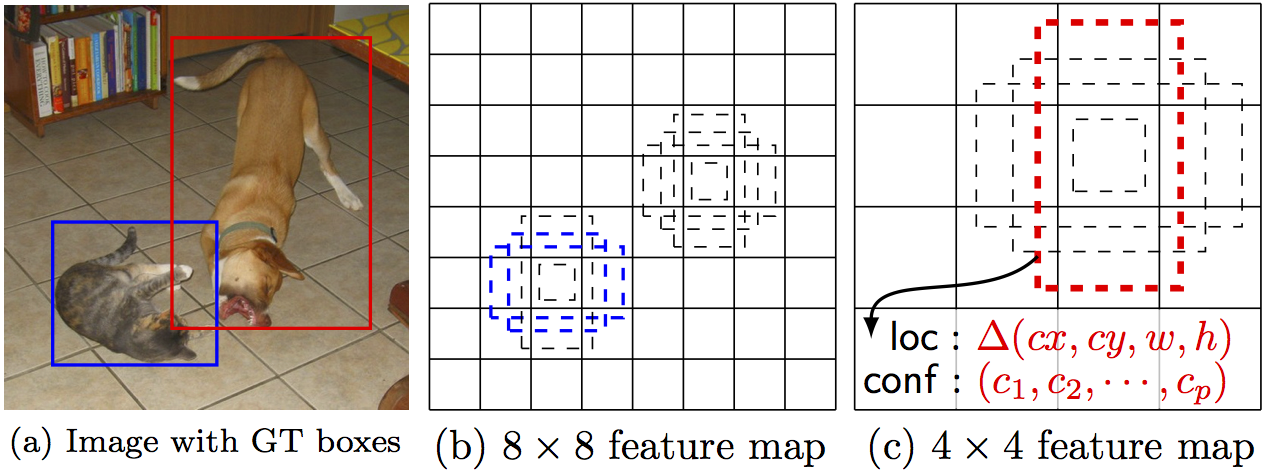
\includegraphics[width=3.5in]{images/ssd_generated_boxes}
				\caption{A set of boxes are generated centered on each point of every feature map \cite{ssd-paper}.}
				\label{fig:5_ssd_generated_boxes}
			\end{figure}
			
			After this, these \emph{priors} are convolved with small filters (one per depth channel), which outputs \emph{softmaxed confidence values for each known class}, and \emph{offsets/adjustments for the generated bounding box}. So, for each detected object (on that scale), we know the score for each class and its estimated position inside the feature map.
			
			\item \emph{Postprocessor}: this element does not appear in \autoref{fig:5_objectdetector_graph}, it had to be cropped on the image for geometrical reasons, but it is present on the network structure. It combines the output of all the 6 \emph{Box Predictors} (which contain detections for each feature map set), and applies a \emph{Non-Maximum Suppresor}, which only retains the most confident detections, and scales its position to the original image size.
		\end{enumerate}
	
	This way, we have a system that, for each introduced image, returns a collection of:
	\begin{itemize}
		\item \emph{Classes}: the detected class (person, cell phone, airplane, dog...) inferred.
		\item \emph{Scores}: the confidence $\in [0,1]$ the network has on each object belonging to the decided class (which was the most probable one while the detection was performed).
		\item \emph{Boxes}: the coordinates of the \emph{bounding box} which wraps the detected object, typically expressed as the coordinates of its top-left and bottom-right corners.
	\end{itemize}
	
	As this is suitable for real-time performance, we are now capable, on a standard computer hardware, to feed it with a video streaming (a file, or live camera images).
	
	\subsection{Importing a pretrained model}
		We have mentioned the training process of this kind of CNNs. It is not complicated from the point of view of the entire system (\emph{black box}), it only needs a dataset containing images with classes and \emph{ground truth boxes}\footnote{\emph{Ground truth}: what the network knows to trust, what is told it to be the true position of the object to detect.} (Microsoft's COCO, Pascal VOC, etc.). With these images, the SSD architecture learns to perform a better \emph{regression}, to achieve a better fitting of the boxes with respect to the original ones, evaluating it using the \emph{Jaccard similarity coefficient}, or IoU (\emph{Intersection over Union}). This measure evaluates how good the overlap between true and estimated boxes is (\autoref{fig:5_iou}). Additionally, it performs a standard \emph{back-propagation} process similar to the one we executed on the previous component (\autoref{sec:4_train}).
		
		\begin{figure}[h!]
			\centering
			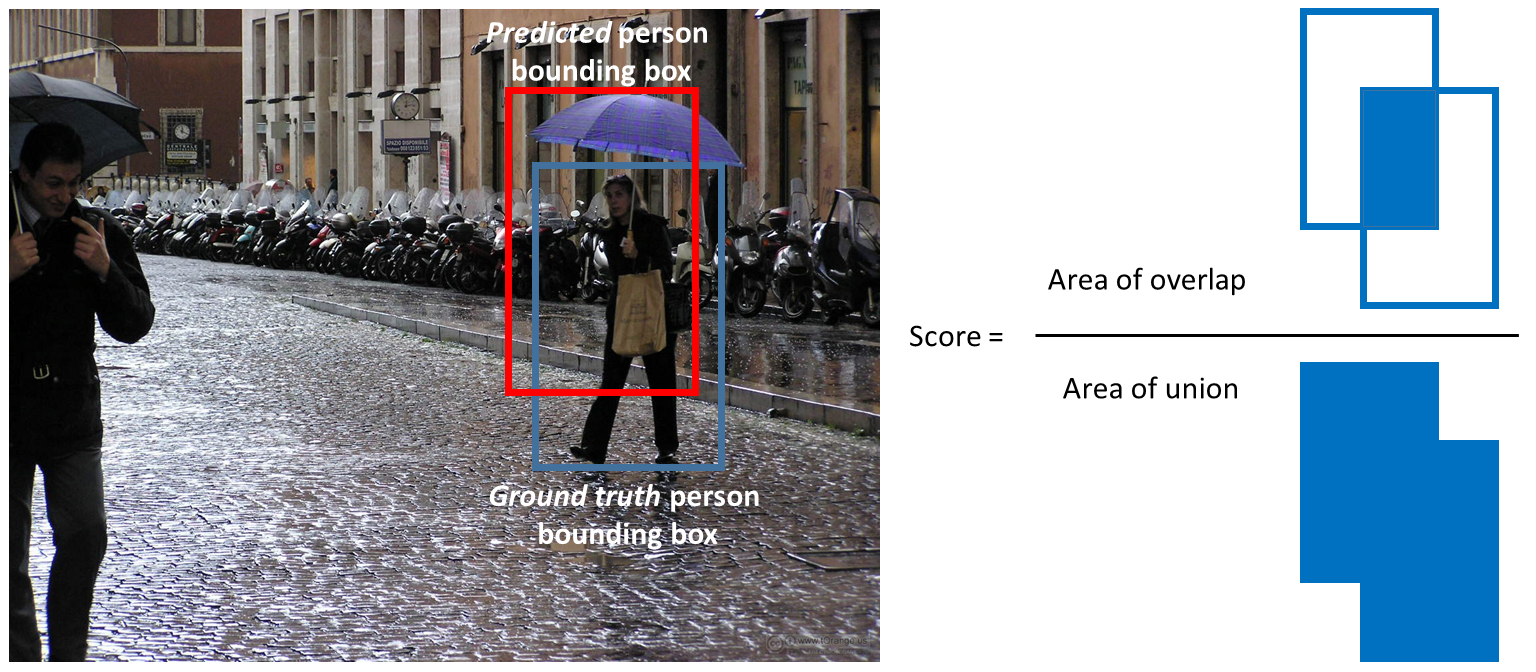
\includegraphics[width=3.7in]{images/detection_iou}
			\caption{\emph{Jaccard similarity coefficient} on a detection (performance indicator used for training a detector).}
			\label{fig:5_iou}
		\end{figure}
	
		The much heavier complexity of this task is not our point where to focus, so we will \emph{embed pretrained models}, available thank to the TensorFlow team on the previously mentioned \emph{Detection Model Zoo}\footnote{\url{https://github.com/tensorflow/models/blob/master/research/object_detection/g3doc/detection_model_zoo.md}}.\\
		
		In our case, we have selected a \emph{SSD detector}, with a \emph{MobileNet v2} feature extraction base network, trained on the \emph{COCO} dataset \footnote{\url{http://cocodataset.org}}. As this dataset support 90 object types (\emph{person, dog, airplane, toothbrush, apple, cellphone, etc.}, those are the classes we are able to detect. It provides a lightweight structure which performs inferences at a framerate of approximately 14 fps (on the currently available hardware).\\
		
		We load this network architecture and weights on the mentioned manner (\autoref{fig:5_load_model}). 
	
	
	\subsection{Network output}
		As we have specified, the detection network yields detected \emph{classes, scores} and \emph{bounding boxes}. Respecting the required asynchronous behavioral, this data is deposited on an accessible zone for the GUI, allowing to begin another iteration when requested.\\
		
		Therefore, as described at \autoref{sec:5_node_architecture} the GUI instance grabs the last detection data the network left on the shared placeholder, and draws it on the visible user interface (\autoref{fig:5_whole_pipeline}).
		
		\begin{figure}[h!]
			\centering
			\includegraphics[width=5in]{images/objectdetector_network_yield}
			\caption{Information flow through the whole pipeline.}
			\label{fig:5_whole_pipeline}
		\end{figure}

\vspace{3.5in}
\section{Experiment: testing different architectures}
	The implemented generic class (\texttt{DetectionNetwork}) allows to load on runtime a pretrained TensorFlow model of neural network. We can take advantage of this to perform a quantitative timing benchmark of different architectures and/or datasets, among the available models on the TensorFlow Detection Zoo\footnote{\url{https://github.com/tensorflow/models/blob/master/research/object_detection/g3doc/detection_model_zoo.md}}. As this node is a implementation on a real time video streaming, measures can't be taken on \emph{precision} terms. However, a deeper analysis of that kind can be performed with the JdeRobot tool \texttt{DetectionSuite} (described on \autoref{sec:dl_jderobot}), which allows to measure performance in terms of advanced markers, as \emph{Jaccard Index}, precision and recall.\\
	
	The timing tests (\autoref{tab:5_tests}) have been performed under the described available hardware (section \ref{sec:2_available_hw}), computing the \emph{mean inference time} over 200 frames on a people walking video (\autoref{fig:5_benchmark_screen}). Notice that the frame rate and/or resolution are not relevant, as the frames are processed one at a time, and experiment a reshaping before being feed-forwarded through the network.
	
	\begin{figure}[h]
		\centering
		
\includegraphics[width=4in]{images/net_benchmarking_screenshot}
		\caption{Screenshot taken from the video used on the benchmark.}
		\label{fig:5_benchmark_screen}
	\end{figure}
	
	
	
	
	\begin{table}[h]
		\centering
		\begin{tabular}{|c|c|c|c|}
			\hline
			\textbf{Architecture} & \textbf{Base network} & \textbf{Dataset} & \textbf{Mean inference time} (ms) \\ \hline
			ResNet  & Inception  & COCO & 820.71 \\ \hline
			SSD  & MobileNet  & COCO & 107.43 \\ \hline
			ResNet  & 101  & COCO & 786.49 \\ \hline
			ResNet  & 50  & COCO & 515.28 \\ \hline
			Inception  & *  & COCO & 349.13 \\ \hline
			ResNet  & 101  & COCO & 63.97 \\ \hline
			Faster-RCNN  & ImageNet  & ILSVRC2014 & 703.99 \\ \hline
			Faster-RCNN  & Inception  & COCO & 352.20 \\ \hline
			ResNet  & 50  & COCO & 793.87 \\ \hline
			*  & MobileNet  & COCO & 106.93 \\ \hline
			SSD  & MobileNet  & COCO & 102.85 \\ \hline
			ResNet  & 101  & COCO & 898.59 \\ \hline
			Inception  & ResNet  & OID & 792.42 \\ \hline
			\textbf{SSD Lite}  & \textbf{MobileNet}  & \textbf{COCO} & \textbf{68.13} \\ \hline
			ResNet  & 101  & Kitti & 111.29 \\ \hline
			Inception  & ResNet  & OID & 667.76 \\ \hline
		\end{tabular}
		\caption{Timing performance tests for several modes. The selected implementation appears in \textbf{boldface}.}
		(*): Not specified.
		\label{tab:5_tests}
	\end{table}
		
	
	
	
	As it can be seen, the vast majority of other implementations (different network architectures) are significantly bigger, which would make impossible to accomplish real-time operation.\\
	
	
	
	
	
	
	
	
	
	
	
	%%%%%%%%% FOLLOW PERSON %%%%%%%%%
	\chapter{\texttt{FollowPerson} node}
\label{chap:followperson}
\section{Description}
	The previous node, \texttt{ObjectDetector}, shows such a fine real-time detection system, for several classes of objects (up to 90 in the COCO dataset case). It conforms an inert node, but that can act as a starting point for a ton of interesting applications to come up with.\\
	
	In our project, we take one of these new derived applications, \texttt{FollowPerson} (\autoref{fig:6_followperson}), and in the next pages we will study its insights. Our approach is a \emph{reactive}\footnote{A reactive action has an immediate effect when the stimulus is perceived.} behavioral on a robot, which commands a Turtlebot robot to follow a target person (which we will call \emph{mom}) using a RGBD\footnote{\emph{RGBD} stands for \emph{RGB + Depth}. It provides, in addition to the standard RGB image, a depth map, as described at \ref{sec:3_xtion}} sensor. This person can be easily specified, providing the node an image of it, in the YML configuration file. The node will search and analyze its faces, and store it as the face to follow. It comprises, as we will see, some new systems as a modular extension of the pure detection component.
	
	\begin{figure}[h]
		\centering
		\includegraphics[width=6in]{images/followperson_working}
		\caption{\texttt{FollowPerson} working (following mom).}
		\label{fig:6_followperson}
	\end{figure}
	
\section{Node architecture}
	On the previous components, we had to support similar tasks, as the only radical change was the inner structure of the neural network. However, on this new component, we have to add a new element to the previous scheme, as we have a new task: \emph{command movements to the wheels of the robot}. This has to be on an independent fashion, according to our design requirements (we can not implement blocking calls, so we need an asynchronous operation). So, the solution to make this possible is simply to implement \emph{another thread}, which will be responsible of controlling the motors, based on the last network output. This way, we will have a schema similar to the one on \autoref{fig:6_followperson_architecture}.
	
	\begin{figure}[h]
		\centering
		\includegraphics[width=5in]{images/followperson_schema}
		\caption{Architecture of the \texttt{FollowPerson} node.}
		\label{fig:6_followperson_architecture}
	\end{figure}
	
	So, as a result, we can count up to 5 different threads:
	\begin{itemize}
		\item \emph{Camera}: as we mentioned, we need the images from a RGBD sensor, which will be provided via ROS (\texttt{OpenNI2}), from the Asus Xtion sensor. These images will be delivered transparently through a ROS topic by the driver, and the Camera object will distribute them to the rest of threads.
		
		\item \emph{Depth}: we obtain a depth map from the sensor, which is also delivered by the \texttt{OpenNI2} driver. One thing to mention here is that, originally, each pixel has a size of 16 bits, standing for the depth in millimeters detected on that particular direction. Unfortunately, through the transport process, it is converted to a 8 bits value, so we lose the real reference of the distance measure. To alleviate this, we will work with \emph{relative} distances, comparing them with the range $[0,255]$ they can take. This is $2^8$ times less accurate, but it is fine given the application and the distance the sensor is capable to reach.
		
		\item \emph{GUI}: this thread is, as before, destined to refresh the visible window, showing the incoming images (RGB image as in \texttt{ObjectDetector}, and depth image, tinted with an artificial \emph{colormap} representing relative distances). 
		
		\item \emph{Network}: it behaves the exact same way than the \texttt{ObjectDetector}'s one, implementing a SSD CNN on a \emph{MobileNet} base network, trained on COCO dataset. The tiny adaptations to this applications will be seen below.
		
		\item \emph{Motors}: this is the new element. It is an asynchronous thread which analyzes the output of the network and, depending on the result of contrasting this information with both received images (RGB and Depth), sends a reactive command to the robot's motors. Even so, it keeps an intermediate tracker to soften the physical response, as it will be explained later.
	\end{itemize}
	
	
\section{SSD CNN Modifications}
	As said, the underlying CNN bundled on this component is the same SSD detector that \texttt{ObjectDetector} uses. However, a subtle modification of its output is performed before making it available to the GUI.\\
	
	As our main objective in this node is to \emph{follow a person}, we are not very interested in detecting other kind of objects in the image. In consequence, we perform a small filtering of the tensors returned by the output layer (\texttt{boxes}, \texttt{scores}, \texttt{predictions}):
	
	\begin{lstlisting}
...

(boxes, scores, detections, _) = self.sess.run([........])
# Now the last layer output is contained in those numpy tensors,
# We will work with the detection indices
# (they are identically sorted in the tensors).

# Firstly, we get the mask corresponding to the most confident
# predictions (to avoid false positives):
mask1 = scores > 0.5
# Then, we get the human detection indices:
mask2 = np.where(detections == 'person')

# Now we combine both masks:
mask = np.logical_and(mask1, mask2)

# And retrieve the most confident human detections,
# (their location and score).
correct_boxes = boxes[mask]
correct_scores = scores[mask]

...
	\end{lstlisting}
	
	Later, as it was done in the detection node, these filtered values are deposited in the accessible placeholder for \texttt{GUI} and \texttt{Motors} components.
\section{Face detection and identification}
	The person following task can be already addressed, but our main interest is to be capable of tracking and following a single person.
	
	\begin{figure}[h]
		\centering
		\includegraphics[width=4in]{images/followperson_pulp}
		\caption{Who should we follow? Probably none of them.}
		\label{fig:6_followperson_pulp}
	\end{figure}
	
	We discern which one is the target person (\emph{mom}), \emph{identifying its face}. To do this, we have to firstly \emph{detect} faces on the image, and then perform a \emph{reidentification} with each found face, to contrast wether that person is or not mom. Now, we will describe the pipeline followed to perform these actions.
	
	\subsection{Detection: Haar Cascade Classifier}
	
		The face detection task has to be performed on the first place, and the chosen approach for this is the one described in \cite{cawadallah}. This face detection algorithm, which is one of the most popular face detection Machine Learning techniques, comprises \emph{Haar features}. The reason for this choice is the lower computational load\footnote{We must remember that this will be running simultaneously with the SSD detector.} it supposes compared to other techniques, as it works with \emph{grayscale images} (simpler than RGB ones), and the specification we have chosen is a simple algebraic computation with the pixel values, which result on a low-complexity system.\\
		
		\emph{Haar features} are binary \emph{masks} (\autoref{fig:6_haar_feats}) that are slided through the \emph{grayscaled} image. On each stride of a particular kernel/mask, the pixels contained on the black zone of the kernel are subtracted from those contained in the white zone (\autoref{fig:6_haar_on_face}). The total result of these convolutions lets us know a promising zone to contain a face, or a clearly negative zone to discard. This takes benefit from the fact that practically on every situation, some determined regions of a human face are darker than others. Hence, certain kernel dispositions will work much better on a determined zone of the face (\autoref{fig:6_haar_on_face}).
		
		As it can be figured, these \emph{Haar} features are not trivial, they are obtained in a training, as a result of a ton of positive (and negative) examples analysis.\\
	
		\begin{figure}[h]
			\centering
			\begin{subfigure}[b]{0.4\textwidth}
				\centering
				\includegraphics[width=3in]{images/haar_features}
				\caption{Haar features.}
				\label{fig:6_haar_feats}
			\end{subfigure}
			\hspace{1in}
			\begin{subfigure}[b]{0.4\textwidth}
				\centering
				\includegraphics[width=3in]{images/haar_on_face}
				\caption{Application of a Haar feature on a face image.}
				\label{fig:6_haar_on_face}
			\end{subfigure}
			\caption{\emph{Haar} features.}
		\end{figure}
		
		
		Once we know what a \emph{Haar} feature is, we can describe the selected algorithm to perform the face detection: a \emph{Haar-like feature Cascade Classifier}. This method, proposed on \cite{haar-cascade} by Viola and Jones, describes a pipeline to process an image, which consists on a \emph{serie} of \emph{Haar-based} checks.\\
		
		The first stages check different areas of the image, using very simple \emph{Haar} features, with the objective to discard regions (\emph{sub-windows}) where certainly there is not a face. Those regions which pass the pixel subtraction test go forward to the next stage, where the process is repeated with a slightly more complex kernel (\autoref{fig:6_cascade_pipeline}). On the final stages, where only a small region of the image could have passed all the previous \emph{Haar} features, the most complex kernels (\autoref{fig:6_haar_complexity}) are applied, discarding the possible false positives, and obtaining, finally, the regions where the system is sure of having detected a face.\\
		
	\begin{figure}[h]
		\centering
		\begin{subfigure}[b]{0.4\linewidth}
			\centering
			\includegraphics[width=3in]{images/cascade_classifier_pipeline}
			\caption{Logical pipeline}
			\label{fig:6_cascade_pipeline}
		\end{subfigure}
		\hfill
		\begin{subfigure}[b]{0.4\linewidth}
			\centering
			\includegraphics[width=2.5in]{images/haar_complexity}
			\caption{Increasing complexity of successive \emph{Haar} features.}
			\label{fig:6_haar_complexity}
		\end{subfigure}
		\caption{\emph{Haar-like feature Cascade Classifier.}}
		\label{fig:6_haar_cascade}
	\end{figure}	
	
		
		Additionally, we can parameterize this detection process by the desired range of sizes to consider on a face, and the minimum number of neighbor features passed to consider a region as a candidate. We validated this system with good results in comparison to other classifiers (as LBP (\emph{Local Binary Patters}) based), but this is the one which yields the best trade-off between satisfactory detections and a low computational load. This last factor is alleviated in some way, because we don't perform the face detection process on all the images, but \emph{only in the currently detected persons}, hence it turns on a much lighter and efficient task that our real-time system can afford. Also, this allows us to keep a limp detection thresholds: if we obtain more than one face in a particular person, we will keep the highest one (as the face detection is constrained inside the person image). The handicap of this kind of classifiers is the difficulty to detect faces on a profile pose, as these features only apply to \emph{frontal face} faces.\\
		
		The way to implement this system has been a OpenCV class, \texttt{cv2.CascadeClassifier}, fed with an XML containing the description of the stages (obtained on a training process and publicly available on OpenCV's official GitHub repository\footnote{\url{https://github.com/opencv/opencv/tree/master/data/haarcascades}}).
	
	\subsection{Face Validation: FaceNet}
		If we have achieved to locate a person's face (it is not always possible since ambient conditions can be harsh sometimes), we can \emph{reidentify it}. We will not deploy a identity storage system, or similar, as it is out of the scope of this node. Instead, we will use a \emph{validation} system to check whether that particular person corresponds to the target to be followed.\\
		
		We have implemented a solution based in \cite{facenet}, which develops a system called \emph{FaceNet}. Its main functionality is to \emph{map} face images to a 128-dimensional Euclidean space, where faces are represented by what is called \emph{embeddings} (feature vectors on this specific space), and the distance between these embeddings directly represents \emph{similarity between the faces}. This way, actions like face recognition, verification and clustering can become immediate, as they can be performed just over the obtained embeddings of each face. The mathematical definition of \emph{distance} is the Euclidean generic one:
		\begin{equation}
			d(\vec{f_1}, \vec{f_2}) = \sqrt{\sum_{i=1}^{128}(f_{1_i} - f_{2_i})^2}
			\label{eqn:6_l2}
		\end{equation}
		
		The advantage of this system in comparison with other approaches relies on the fact that it offers \emph{strength}, as it runs a deep neural network underneath: the embeddings are optimized through a standard training process (using Stochastic Gradient Descent, with batches of tenths to hundreds of examples\footnote{Again, we can notice that it is a simple process in comparison with non-deep-learning techniques, since we only need images of the faces labeled with their identity.}), based on a particular cost function, called \emph{triplet loss} (\autoref{fig:6_facenet_triplet_loss}). What is achieved is a minimum distance between the computed embeddings for images of the same face, and a maximum distance between faces of different individuals. This makes of it a really robust system, since these kind of networks, trained with images on different lighting and pose conditions, offer an excellent performance on real environments. In addition, it is a simple system, as the resultant embeddings are just 128-bytes values (easier to handle than other state-of-the-art system which implement PCA analysis, SVM classifications, etc.). Some other approaches, as \emph{siamese networks} consist on a real-time comparison between two faces. This would make less sense in this scenario, as we will compare the current face with a \emph{static} one, so it would be a waste of efficiency to compute the same values all the time for the reference face (\emph{mom's}).\\

		
		\begin{figure}[h]
			\centering
			\includegraphics[width=4in]{images/facenet_triplet_loss}
			\caption{Triplet loss training. It minimizes the distance between an \emph{anchor} (current example) and a \emph{positive}, both of which have the same identity, and maximizes the distance between the \emph{anchor} and a \emph{negative} of a different identity (from \cite{facenet}).}
			\label{fig:6_facenet_triplet_loss}
		\end{figure}
		To sum up, we can appreciate that this is another perfectly suitable scenario for deep-learning, where it can perform much better in efficiency and simplicity\footnote{Perfectly compliant with \emph{KISS} principle: \url{https://en.wikipedia.org/wiki/KISS\_principle}} than other approaches.\\
		
		The objective implementation\footnote{Inspired on:  \url{https://github.com/davidsandberg/facenet}} on this node is achieved, as with previous detection networks, with the \emph{generic TensorFlow model loading}. We recover the graph and weights stored in the \texttt{.pb} model pretrained on the source repository (on the footer of this page), represented on \autoref{fig:6_facenet_tensorboard}. As it can be seen, its structure is such a simple one.
		
		\begin{figure}[h]
			\centering
			\includegraphics[width=2in]{images/facenet_tensorboard}
			\caption{\emph{FaceNet} architecture.}
			\label{fig:6_facenet_tensorboard}
		\end{figure}

 Additionally, to ensure a robust response under different environment conditions, we include a preprocessing phase for every image entering to the network:
 \begin{enumerate}
 	\item \emph{Reshape}: the imported network works with 160$\times$160 face images, so we have to resize the face to that particular shape.
 	
 	\item \emph{Blur} (with a small kernel): this is applied due to the probable low resolution and high noise that the analyzed face can suffer. It has to be kept in mind that the camera will be situated near the floor, looking upwards. This will cause the face to have a far position with respect to the sensor.
 	
 	\item \emph{Prewhiten}: with the objective of being insensible to light conditions of the image, we perform a normalization process of the face, eliminating the light information. This is achieved with a standard normalization operation on each color channel, being $x$ the matrix of that channel of the image, $\mu$ its mean and $\sigma$ its standard deviation:
 	\begin{equation}
	 	x' = \frac{x - \mu}{\sigma}
 	\end{equation}
 	
 	So, we obtain a normalized image, which is centered on $0$ and scaled on a same way (by its standard deviation). We achieve much more comparable images with this method.
 \end{enumerate}
 
 The final result of this preprocessing pipeline can be observed at \autoref{fig:6_preprocessing}, where we obtain the normalized faces, ready to be processed by the \emph{FaceNet}, which will compute the embeddings. We can compute the resulting $L^2$ Euclidean distance (\autoref{eqn:6_l2}), through the methods we have implemented on the \texttt{FaceNet} class:
 
 \begin{lstlisting}
...
img1 = imread('img1.jpg')
img2 = imread('img2.jpg')

# We discard the second output (it contains the face bounding box).
face1, _ = facenet.getFace(img1)
face2, _ = facenet.getFace(img2)
# The next method performs the face preprocessing, feed-forward pass of
# both faces, and compute the distance.
distance = facenet.compareFaces(face1, face2)
...
 \end{lstlisting}
 
 \begin{figure}[h]
 	\centering
 	\includegraphics[width=5in]{images/facenet_prewhiten}
 	\caption{Preprocessing result on several conditions (the different colors in the output images are due to the color mapping performed by the plotting backend), and $L^2$ distances computed between the faces.}
 	\label{fig:6_preprocessing}
 \end{figure}
 
 The last thing to do is establish a \emph{threshold} distance, to decide whether the two compared faces are the same or not. The experimental tests drove us to the same values that the paper \cite{facenet} specifies: a distance threshold of $1.1$ (notice that at \autoref{fig:6_preprocessing}) the three faces have a respective distance between them below that threshold, because they belong to the same person, even at different lighting conditions as it can be appreciated.\\
 
 As we mentioned before, we will use this small deep neural network to compare all found faces with \emph{mom}'s (which will be a constant, as it comes from the reference image provided to the node). So, first of all, we compute \emph{once} \emph{mom}'s embeddings, and compare the live obtained embeddings from new found faces with \emph{mom}'s, just computing the distance between them. As this is a methodical task, it has been included as another method inside the class: \texttt{compareWithMom(face)}.
 
\section{Face and Person Trackers}
	So far, we are able to detect the seen persons in the image, and the faces inside these persons. After completing these two process successfully, we are ready to compare a certain face with \emph{mom}'s. However, although the person detection CNN is extremely robust (which is its main advantage), it can miss a detection sometimes, because of the lighting or confusing environment around the person. On the other hand, the face detection algorithm (\emph{Haar-like feature Cascade Classifier}) is more susceptible to failure, as it is a simple (although efficient) method, which is not designed for difficult situations. This is as alleviated as possible inside the detection pipeline\footnote{As we mentioned before, we have implemented a very limp detection conditions, filtering the detected faces and keeping the highest one.}, but \emph{false positives} are feasible even so.\\
	
	For this reason, we have inserted an \emph{intermediate} block between the detection algorithms (person, face), and the face validation: the \emph{trackers}. These trackers are a security measure to avoid false positives and false negatives. As its operation is the same in both cases (persons and faces), we will describe it on the generic case, working with \emph{instances}, and concretely with its bounding boxes (which determine its position).\\
	
	The tracker divides the instances into three sets:
	\begin{itemize}
		\item \emph{Detected instances}: the fresh instances which have just been detected in the image (\texttt{DetectionNetwork} or \texttt{CascadeClassifier}).
		
		\item \emph{Candidate instances}: the detected instances which are during the process of being a tracked one.
		
		\item \emph{Tracked instances}: the candidate instances which have passed a period of \emph{patience}, and are currently being tracked. These are those we will consider to look for \emph{mom} and/or compute a physical response. If we lose these instances we will keep thinking for a marginal lapse of time that it is still there.
	\end{itemize}
	
	This way, we are not trusting directly the raw output from the detectors, but trusting instead the combination of that output with the past detections. We will avoid \emph{false positives}, as \emph{detections} will have to be for a while on the \emph{candidate} set, and we will also false negatives, as \emph{tracked} instances will stay for a while in that set even if they are not detected, before being untracked. So, \emph{our movements will be dictated by the tracked stimuli, not by the detected ones}. This will eliminate noisy responses and get a much softer behavioral than trusting directly the imperfect output from a classifier.
	
	Its operation and exchanges between sets is the same in both cases (person and face), using a counter (owned by each instance) that is varies between 0 and the patience value (we have set 5 as a prudent number):
	
	\begin{enumerate}
		\item When a new instance is detected, its position goes into the \emph{detected} set.
		
		\item Its position is compared\footnote{All the distance comparations between instances are made computing the module of the distance vector (in px) between their centers.} with each \emph{tracked} instances. If it is suspiciously near of a \emph{tracked} instance, it is taken as the new detection for that instance. So, the \emph{tracked} instance position is updated (taking the new value), and its counter is incremented in 2 units. The \emph{detected} instance is removed of the \emph{detected} set.
		
		\item If it does not belong to any \emph{tracked} instance, we try the same for the \emph{candidate} instances. If we are successful with one of them, this \emph{detected} instance is taken as the new position for that \emph{candidate} one, so its position is updated and its counter is incremented in 2 units. The \emph{detected} instance is removed of the \emph{detected} set.
		
		\item If we were not successful in any of the previous cases, this instance is a completely new detection, so it is appended to the \emph{candidate} set (with a counter value of 1), where it will stay for a while if it keeps being detected.
	\end{enumerate}

	This described procedure is repeated with every new detection. When it has finished, before ending the iteration, a \emph{general update} is performed over all the \emph{candidate} and \emph{tracked} instances:
	
	\begin{enumerate}
		\item The counter of all the \emph{candidate} instances is checked. If it has reached the patience value, it is considered that it has been seen for too much time for being a false positive, so it goes into the \emph{tracked} instances (with a counter equal to the patience + 1).
		
		\item If any of the \emph{candidate} instances has reached 0 on its counter, that means that it has not been detected anymore, so it was a false positive (it was not detected long enough to move to the \emph{tracked set}). It is removed from the \emph{candidate} set.
		
		\item The same step for the \emph{tracked} instances: if any of them has reached 0 on its counter, it is removed (it was a \emph{tracked} instance which has been lost for enough time for not being considered a false negative).
		
		\item The counter for all the \emph{tracked} and \emph{candidate} instances is decremented in 1.
	\end{enumerate}
	When a strong detection is mantained, it is stored in the \emph{tracked} set, and its counter is always saturated to the maximum value, so it is safe for being demoted for a while if it stops being detected for a few frames. This can be applied to person detections (avoiding undesired detections) and to face detections (this cancels the effect of the limp face detection, where only the highest one will be kept and, in addition, it will have to be detected for a few frames to be considered).\\
	
	This role promotion and demotion system is successfully implemented with custom types in Python, where we have a general \texttt{PersonTracker}, which keeps the coherence between the sets for all the image, and a \texttt{FaceTracker} inside each person (to have three of the explained sets being executed for each detected person) yielding excellent results to keep steady detections. This allows to handle faces only inside detected persons (which also eliminates false positive face detections outside a person, which is never convenient).\\
	
	The general effect of the inertia provided to the confident detections allows to have a much softer response in case of fleeting false positives/negatives. We can have a glance on this behavioral on \autoref{fig:6_trackers}.
	
	\begin{figure}[h]
		\centering
		\begin{subfigure}[b]{0.4\linewidth}
			\centering
			\includegraphics[width=3in]{images/person_tracker}
			\caption{Tracking process for a person.}
			\label{fig:6_person_tracker}
		\end{subfigure}
		\hfill
		\begin{subfigure}[b]{0.4\linewidth}
			\centering
			\includegraphics[width=3in]{images/face_tracker}
			\caption{Tracking process for a face.}
			\label{fig:6_face_tracker}
		\end{subfigure}
		\caption{Schema followed by the trackers.}
		\label{fig:6_trackers}
	\end{figure}

\section{Physical response}

		The main objective of this node is to \emph{command movements to the Turtlebot motors}. We need to know how to behave, and which will be the good movements to command to arrive to \emph{mom}'s position.
		
	\subsection{Follow algorithm}
		
		\begin{wrapfigure}{r}{7cm}
			\centering
			\includegraphics[width=7cm]{images/followperson_flowchart_cropped}
			\caption{Following behavioral (flow chart).}
			\label{fig:6_followperson_flow_chart}
		\end{wrapfigure}
		Once we have detected, tracked and identified \emph{mom}, we have to keep a certain intelligence, or behavioral schema, to know what to do on each possible scenario. The \emph{flow chart} of the implemented behavioral is represented on \autoref{fig:6_followperson_flow_chart}, where we can see that \emph{it is enough for us to identify mom once}. Given that it will be tracked, we can automatically update its position,  without the need to see its face again to confirm that it is mom indeed. If we are following mom without seeing its face, and we find its face on another detected person, the role of \emph{mom} will swap to this new person, who will be followed from that moment.\\

		In last place, if we don't see \emph{mom} our robot stays in its place, slowly turning towards last \emph{mom} tracked position, in order to find it again.

	\subsection{Position calculation}
		The fact of knowing, thank to  all the previous blocks, where \emph{mom} is inside the image lets us know where (relatively to the robot) it is, given that the RGBD sensor is aligned with the Turtlebot frontal face. This means that, what is seen along the center of the image will be just in front of the robot, on a straight line. Thus, we will be able to act in consequence on both of the motors interfaces that the Turtlebot offers:
		
		\begin{itemize}
			\item \emph{Angular}: the first thing we have to figure out is if the robot has to rotate towards \emph{mom}. This can be computed with the bare \emph{mom}'s bounding box. If we compute its center, we can know the horizontal distance from it to the entire image center. This will give us the \emph{horizontal error} (measured in pixels, as it is a relative amount) (\autoref{fig:6_h_error}).
			
			\item \emph{Distance}: the other error to compute is the distance one. This one is figured out on a slightly different way. As explained at \autoref{sec:3_xtion}, a \emph{registration} process carried out by the driver maps the depth pixels into the RGB ones. So, if we know \emph{mom}'s position in the RGB image (its bounding box), \emph{its depth measures will be right inside the same box in the depth image}. That is the source of the measure. The implemented approach to obtain a single value (as we need it to send the proper command to the motors) is to perform a \emph{spatial depth sampling} inside the depth slice, cropped with the bounding box. To be cautious, we keep the depth image inside a safety margin of 10\% of the image (to be sure we sample inside the person). Then, we create a 10$\times$10 \emph{grid} inside this new crop, and retrieve the depth values measured on those points (a total of 100 measures). The total estimated distance will be the median\footnote{We choose the median for being generally more robust than the mean, as it is not affected by the value of outlier measures (an accidental sample on a background surface would alter the mean on a significant way).} of that set of measures (\autoref{fig:6_distance_to_mom}).
		\end{itemize}
		
		\begin{figure}[h]
			\centering
				\begin{subfigure}[b]{0.4\linewidth}
				\centering
				\includegraphics[width=3in]{images/h_error}
				\caption{Horizontal error estimation.}
				\label{fig:6_h_error}
			\end{subfigure}
			\hfill
			\begin{subfigure}[b]{0.5\linewidth}
				\centering
				\includegraphics[width=3.7in]{images/distance_error}
				\caption{Computation of the median distance to \emph{mom}.}
				\label{fig:6_distance_to_mom}
			\end{subfigure}

			\caption{Computations of both errors.}
			\label{fig:6_errors}
		\end{figure}

	
	
	
	\subsection{PID controller}
		Once we know the relative \emph{mom}'s relative position from the robot, we have to send the proper commands to the robot, to make it follow \emph{mom}. On the first place, we have to know when to act and when to stop the motors. As we don't want the robot to go to the exact place where \emph{mom} is, we have to establish a \emph{safe/dead zones}, where we the robot won't move further towards \emph{mom}. These zones are represented in \autoref{fig:6_followperson_safe_zones}.\\
		
		\begin{figure}[h]
			\centering
			\includegraphics[width=4in]{images/followperson_movement_schema}
			\caption{Safe zones. The robot will consider \emph{mom} as correctly followed inside them (on a separate way for each dimension).}
			\label{fig:6_followperson_safe_zones}
		\end{figure}
	
			As our desirable relative position is to be aligned (the center of the bounding box in the center of the image) and at a safe distance (at $\pm$ 10 px from the reference distance), we will rotate and/or move in a straight line in consequence, trying to carry \emph{mom} inside the safe zones. Hence, we have to \emph{compute a proper response} to move the robot towards the correct direction (independent responses on the angular and linear dimensions). Instead of computing just a response on a proportional way to the current error, we can implement a \emph{closed loop feedback system}, which keeps in mind the previous readings and responses computed, to get a better fitting to the ideal response in that moment\footnote{Otherwise, we can suffer oscillations and peaks on the response, as this application is a system affected by noise and possible errors in the measure. That is the reason why we implemented all the past softening blocks.}. Concretely, we will implement a \emph{PID} controller \cite{pid:}, which is the most common form of feedback at industrial applications (more than 95\% of the control loops are of this kind). PID stands for \emph{Proportional, Integral and Derivative} control, and computes a total response ($u(t)$) following the next formula (modified for discrete time, as we are on a digital system):
			
			\begin{equation}
			u[n] = k_p e[n] \ \ + \ \ k_i \sum_{i=0}^{n}e[i] \ \ + \ \ k_d (e[n] - e[n-1])
			\label{eq:6_pid}
			\end{equation}
			
			For those who did not stop reading, we will analyze this formula, which combines three sub-responses:
			
			\begin{itemize}
				\item \emph{Proportional}: $k_p e[n]$. This is the basic component, that computes a response directly proportional to the measured error.
				
				\item \emph{Integral}: $k_i \sum_{i=0}^{n}e[i]$. Here we compute an additional response, equivalent to the summation of the total error until now. This way, although a proportional response is not enough and the error gets stabilized in a non-zero value, the system will accumulate that error, getting \emph{annoyed} with the time. So, we will get a bigger response the bigger the total error is\footnote{When the monitored variable goes into the tolerated zone again, the total error has to be reseted, as it won't be necessary for now.}.
				
				\item \emph{Derivative}: $k_d (e[n] - e[n-1])$. This part stands for the \emph{difference} between the last measured error and the current one, and it quantifies how is the system responding\footnote{On systems without inertia, this contribution is generally ignored, having a simple PI control loop instead.}. If the difference has a high value, that means that the system is on a far state/position with respect to the last iteration. So, in order to eliminate the \emph{inertia} the system could have acquired (which might bring oscillations and overshooting), the derivative part acts, braking or accelerating the command depending on the observed response to the previous one.
			\end{itemize}
			
			As we can see, the combination of the three responses can achieve a much faster and steadier response (\autoref{fig:6_pids}), bringing back the system under control on a fast and efficient way. Each contribution is parameterized by its corresponding constant ($k_c, k_i, k_d$), so a critical task is to find the optimum value for each one of them.\\
			
			For our implementation, as we have implemented two independent PID controllers (for linear and angular speeds, respectively), we have experimentally looked for the most suitable values for each one of the parameters, obtaining the combination on \autoref{tab:6_pids}. It is important to mention that these are not the final values that regulate the movement (as the angular and linear errors move in different scales, a difference of 1 pixel in the angular error means almost nothing, but much more in the linear one). For this reason, and to keep reasonable values, they are scaled by internal constants inside of each PID controller.
			
			\begin{table}[h]
				\centering
				\begin{tabular}{|c|c|c|}
					\hline
					\textbf{} & \textbf{Linear} & \textbf{Angular} \\ \hline
					$k_p$     & 2               & 7                \\ \hline
					$k_d$     & 0.1             & 0.5              \\ \hline
					$k_i$     & 3               & 10               \\ \hline
				\end{tabular}
				\caption{Optimal found values for the parameters in each PID controller.}
				\label{tab:6_pids}
			\end{table}
			
			As the rule that governs the controller is the same (\autoref{eq:6_pid}), we have created a generic class (\texttt{PIDDriver}), which controls a motor with a PID closed loop, adding extra functionalities as soft reactive responses (to avoid abrupt movements), and limiters in the response, to mantain control over the robot.\\
			
			
			
			
			 \begin{figure}[h]
			 	\centering
			 	\begin{subfigure}[b]{0.3\linewidth}
			 		\centering
			 		\includegraphics[width=2.2in]{images/pid_p}
			 		\caption{Proportional.}
			 		\label{fig:6_pid_p}
			 	\end{subfigure}
			 	\hfill
			 	\begin{subfigure}[b]{0.3\linewidth}
			 		\centering
			 		\includegraphics[width=2.2in]{images/pid_pi}
			 		\caption{PI.}
			 		\label{fig:6_pid_pi}
			 	\end{subfigure}
			 	\hfill
			 	\begin{subfigure}[b]{0.3\linewidth}
			 		\centering
			 		\includegraphics[width=2.2in]{images/pid_pid}
			 		\caption{Full PID.}
			 		\label{fig:6_pid_pid}
			 	\end{subfigure}
			 	\caption{Different controllers response along time.}
			 	\label{fig:6_pids}		 	
			 \end{figure}
		
	This way, we compute a suitable response with a PID controller for each dimension, and the mentioned class sends it directly to the motors (thank to the possibility of passing the move function as an argument to the generic controller).\\
	
	So finally, we have the final code schema of the functionality added in top of \emph{ObjectDetector}:
	
	
	\begin{lstlisting}
...
# jdrc is the comm communicator.

# We create the client to move the robot:
motors_publisher = jdrc.getMotorsClient('FollowPerson.Motors')
w_function = motors_publisher.motors.sendW
v_function = motors_publisher.motors.sendVX

# Controllers creation:
w_PID = PIDController(w_function,
                      Kp=_,
                      Ki=_,
                      Kd=_,
                      scaling_factor=_,
                      limiter=_)

w_PID = PIDController(w_function,
                      Kp=_,
                      Ki=_,
                      Kd=_,
                      scaling_factor=_,
                      limiter=_)
...

# Measure of the errors:
angular_error = [subtract centers]
linear_error = [sample depth of person]

# Computation of the response (PID controllers):
w = w_PID.computeResponse(angular_error)
v = v_PID.computeResponse(linear_error)

# The controllers automatically send the response on a
# reactive but soft way.
	\end{lstlisting}

	At the end of the each iteration, we get the robot moved towards \emph{mom} (the target person to follow), making use of all the previously defined blocks (\autoref{fig:6_followperson_final}), as it can be seen on the final result, posted on the project Wiki\footnote{\url{http://jderobot.org/Naxvm-tfg}}.


	\begin{figure}[h]
		\centering
		\includegraphics[width=5in]{images/followperson_general_schema}
		\caption{Functional diagram of the \texttt{FollowPerson} node.}
		\label{fig:6_followperson_final}
	\end{figure}

\section{Experiment: PTZ Camera}
	\label{sec:follow_ptz}
	As an alternative experiment or approach, we can implement this tracking and following system on a PTZ camera. As explained in \autoref{sec:3_ptz}, these cameras are supported by servo motors on vertical and horizontal axis, that allow the camera to move as a \emph{mechanical neck}.\\
	
	We can consider an alternative system, which implements the previous pipeline (with slight modifications), using this camera (Sony EVI D100P, on \autoref{fig:3_evi}) as the \emph{actuator device}. Thank to the Python distribution easiness using packages, this case can be implemented as an additional package, being able to modify as less as possible. So, \texttt{FollowPerson} commutes pertinent functions between the Turtlebot and the PTZ packages in runtime, just selecting the used device in the YML file.\\
	
	The movement commands are now destinated to pure \emph{rotations} of the neck, so the movement update on each axis (vertical/horizontal) has to be computed on a similar way than the horizontal case on the Turtlebot (\autoref{fig:6_h_error}). So, our approach in this case follows the computation on \autoref{fig:6_ptz_error}
	
	
	\begin{figure}[h]
		\centering
		\begin{subfigure}[b]{0.6\linewidth}
			\centering
			\includegraphics[width=4in]{images/ptz_error_comp}
			\caption{Error computation on each axis.}
			\label{fig:6_ptz_error}
		\end{subfigure}
		\hfill
		\begin{subfigure}[b]{0.5\linewidth}
			\centering
			\includegraphics[width=4in]{images/ptz_dead_zone}
			\caption{Dead zone of actuation (radius of 60 px).}
			\label{fig:6_ptz_dead_zone}
		\end{subfigure}
		\caption{Error computation parameters on the PTZ case.}
		\label{fig:6_ptz_parameters}
	\end{figure}
	
	However, as the movement commands are stored in a queue buffer, we are limited to perform \emph{differential} pose updates (e.g. move 1 or 2 degrees on each axis towards the objective per iteration), as described in \autoref{fig:3_ptz_movements}. Hence, a PID controller does not make sense here, as the set of feasible outputs is discrete and non adjustable:
	\begin{itemize}
		\item $0$ if the error stays inside the dead zone (\autoref{fig:6_ptz_dead_zone}).
		
		\item $\pm 1$ if the system lost \emph{mom} (in order to slowly move looking for it).
		
		\item $\pm 2$ if mom is being tracked. The camera performs an increment of that magnitude towards mom in each axis.
	\end{itemize}
	

	Finally, we can take advantage of the most of the standard \texttt{FollowPerson} total algorithm, obtaining the schematic algorithm on \autoref{fig:6_ptz_total}.
	
	
	\begin{figure}[h]
		\centering
		\includegraphics[width=5.5in]{images/ptz_general_schema}
		\caption{Total schema followed in the PTZ case.}
		\label{fig:6_ptz_total}
	\end{figure}
	
	
	%%%%%%%%% CONCLUSIONS %%%%%%%%%%%
	\chapter{Conclusions}
\section{Conclusions}
	This final chapter will be devoted to revisit the  proposed objectives. They could be summarized in a central purpose: \emph{enriching the JdeRobot framework with new tools and applications focused on deep learning}. With a complete coverage of the performed tasks, as it has been described on the previous pages, we can contrast what has been achieved on each milestone which was established along the way, in order to accomplish incremental achievements.\\
	
	\begin{description}
		\item[Classification tool for processing live images.] \hfill
			\vspace{0.2in} \\
			The first objective was to upgrade the scope for an existing JdeRobot tool, \texttt{DigitClassifier}, which was designed to perform \emph{classification} tasks using \emph{deep learning} techniques.\\
			
			Its functionality was extended to support the \emph{deep learning} framework TensorFlow, implementing and training networks on our own. This has allowed to achieve initial knowledge about the framework, and enough skills to move towards more complex tasks.\\
			
			In light of the excellent achieved performance, the brand new TensorFlow implementation and the previous one (made with the Keras framework) were merged into an \emph{official JdeRobot} component\footnote{\url{https://github.com/JdeRobot/dl-digitclassifier}}, capable of commuting between both frameworks.
		
		\item[Neural detection tool for live images.] \hfill
			\vspace{0.2in} \\		
			After having accomplished a basic domain on \emph{deep learning} with \emph{classification} tasks, we tackled a more ambitious milestone: \emph{detecting objects on a real-time operation}. There was no previous reference in the JdeRobot framework.\\
			
			The process of training a detection network was ruled out of the scope of this project, so we addressed the detection task using publicly available \emph{pretrained networks}. So, we developed a wrapping of TensorFlow environment to \emph{abstract} the model (architecture, dataset on which it was trained, output format, etc.), and moved the neural network processing to a \emph{GPU environment} (to achieve the optimum predicting rate for a real-time operation). This remarkably efficient detection framework was demonstrated to be capable of real-time processing, so we have developed an entire node, \texttt{ObjectDetector}, to visually perform this task on an \emph{incoming image stream} (abstracting the source).\\
			
			Hence, the final result  has been a node displaying the raw current image, and aside the same one with the detected objects overlaid, indicating their location making use of \emph{bounding boxes}, in addition to the estimated \emph{class} for the object, and the \emph{score} (standing for the reliability level that estimation has).\\
			
			Once more, the excellent performance on real-time (using detectors with a SSD architecture for instance) has driven us to integrate this node\footnote{\url{https://github.com/JdeRobot/dl-objectdetector}} in the JdeRobot framework as well, developing another module to do the same for Keras network models. This has enabled us again to be able to abstract the frameworks, and toggle one of them through the YML file. In addition, this has given us the capability of \emph{benchmarking} new models, as they can be transparently loaded into the created environment, and begin making inferences on real time.
		
		\item[Tracking and following robot behavior using deep learning detection] \hfill
			\vspace{0.2in} \\
			The two previous milestones allowed us to accomplish \emph{state-of-the-art} purposes in the \emph{Computer Vision} field. As the final research objective, we have considered an \emph{actuation} system which uses a powerful \emph{neural network} to accomplish an robust visual perception. In order to overlap our research with the prosperous field of \emph{robotics}, we have developed a component capable of \emph{following} a specific person (\emph{mom}). This has been achieved using concepts like a \emph{PID} controller feedback control, and case-based control.\\
			
	\end{description}
	
	All these achievements have contributed the JdeRobot framework with an upgraded tool (\emph{DigitClassifier}, which now offers support for both Keras and TensorFlow), a brand new tool (\emph{ObjectDetector}), and a new robotics application (\emph{FollowPerson}, capable of chasing a person with excellent results). These new resources are focused on providing real time operation. In addition, all the underlying software created (the \emph{TensorFlow} and \emph{Keras} generic network loaders) can be of great help for future applications.\\
	
	Beyond the technical contents, this project has allowed an interested person in \emph{deep learning} to learn about a cornucopia of concepts and experience. A while ago, when it was decided to evolve towards creating a reactive behavioral, it was motivating to make the most of a possible synergy between two different fields of knowledge, as \emph{deep learning} and \emph{robotics} are.\\
	
	In the professional point of view, it has been essential to acquire further skills about \emph{version control systems}, as Git. This can be an important benefit, as every development project in a corporate environment makes use of this kind of controls.

\section{Future lines}
	The proposed milestones on this project have been successfully achieved using a useful and innovative tool as \emph{deep learning}. Furthermore, it opens some interesting doors to future research or improvements:
	
	\begin{itemize}
		\item \emph{Upgrade DigitClassifier:} for now, this component looks for the digit in a fixed window inside the input image (the central square). Another module could be implemented to perform a \emph{character detection} in the whole image, maybe an OCR number detector.
		
		\item \emph{Translate the Python nodes to a compiled and fast language:} one of the main handicaps of Python is the fact that it is an interpreted language (much slower than a compiled one). So, a \emph{translation} to a lower level language as \texttt{C++} would be very interesting, as it is a widely supported language in this framework, and there are already very efficient \emph{deep learning} implementations on it (as \emph{Darknet/YOLO}).
		
		\item \emph{Use a deep learning face detector in FollowPerson:} the main advantage of the \emph{deep learning} systems is the robustness on their operation, so a facial detection system implemented with this technology could be a powerful resource to perform a facial detection/validation in harshly lightened environments.
		
		\item \emph{Multimodal person detection/tracking:} some extra functionality could be squeezed from a RGBD sensor, like \emph{tracking a person in complete darkness}. As \emph{deep learning} systems offer good results distinguishing a person silhouette, we could perform people detection on a depth image.
		
		
		\item \emph{Add a navigation algorithm to FollowPerson:} the movement commands sent to the Turtlebot are now decided taking into account only the relative position of the person from the robot. However, as the robot incorporates a laser sensor, we can add an \emph{obstacle avoidance} system, in order to perform a non-blind navigation towards the person.
	\end{itemize}

	%%%%%%%%% BIBLIOGRAPHY %%%%%%%%%
	\bibliography{bibliography}
	\bibliographystyle{unsrt}
\end{document}